


\section{Introduction}
\label{sec:intro}
% ---- ---- ---- ---- ---- ---- ---- ---- ---- ---- ---- ---- ---- ---- ---- ---- ---- ---- ---- ---- ---- ---- ----

The Standard Model (SM) of particle physics successfully describes the
majority of high-energy experimental data~\cite{pdg}. One of the key
remaining questions is the origin of the masses of W and Z bosons.  In
the simplest implementation of the SM, it is attributed to the
spontaneous breaking of electroweak symmetry caused by a new scalar
field.  The existence of the associated field quantum, the Higgs
boson, has yet to be experimentally confirmed.  Therefore, the search
for the Higgs boson is arguably one of the most important studies
being done at the LHC~\cite{lhcmachine}. For Higgs masses above or
near the threshold for decay into two vector bosons, the decay modes
of choice are dominated by those decays because of their large
branching fractions.
It is clear that the events where one $W$ decays leptonically, which
provides the main trigger elements, while the other decays
hadronically have the largest branching fraction and have a
reconstructable Higgs mass peak~\cite{intro2}.

Figure~\ref{fig:higgsXSBR} shows the SM prediction for Higgs
production cross-section at the LHC for several production
modes. Clearly the gluon-gluon fusion production mechanism is dominant
over the entire range shown. We have documented a search for the SM
Higgs boson in the WW$\rightarrow\ell\nu jj$ decay channel in
CMS-AN-2011-110 \cite{CMS-AN-2011-110}, using 2011 data, that was
optimized for gluon-gluon fusion production. This analysis note
focuses on the subdominant production mechanism qq$\rightarrow$Hqq,
otherwise known as the vector boson fusion (VBF) mechanism, since
the initial state quarks radiate two W bosons, which fuse to create
a Higgs boson. The quarks appear in the final state as two ``tag jets''
that exhibit a wide rapidity gap; one or both jets are likely to appear
in the forward region of the detector. Requiring such jets in the object
selection helps to significantly reduce backgrounds that appear in the
gluon-gluon analysis. As one can see from Fig.~\ref{fig:higgsXSBR}, the 
contribution for total Higgs production from VBF increases with the
Higgs mass; therefore we set our sights on higher masses with this
analysis.

This analysis employs heavily the same techniques described in
\cite{CMS-AN-2011-110}; therefore in the interests of brevity we
choose not to duplicate all of the motivation and systematic studies
of that analysis here, but rather reference where convenient and focus
instead on those components that are introduced or modified as
necessary to perform this VBF analysis. Here we treat the overlap from
gluon-gluon events leaking into our VBF selection as a signal
cross-efficiency, in the same manner that \cite{CMS-AN-2011-110}
treated the VBF events as contributing to the total yield from
gluon-gluon production; therefore, by way of warning, one cannot take
the results of the two analyses and simply ``add'' them.

%%%%%%%%%%%%%%%%%%%%%%%%%%%%%%%%%%%%%%%%%%%%%%%%%%%%%%%%%%%%%%%%%%%%%%%%%%%%%%%%%%%%%%%%
%%%%%%%%%%%%%%%%%%%%%%%%%%%%%%%%%%%%%%%%%%%%%%%%%%%%%%%%%%%%%%%%%%%%%%%%%%%%%%%%%%%%%%%%
%%%%%%%%%%%%%%%%%%%%%%%%%%%%%%%%%%%%%%%%%%%%%%%%%%%%%%%%%%%%%%%%%%%%%%%%%%%%%%%%%%%%%%%%
\section{Signal and background expectations from CMS simulation}
\label{sec:MCexpectations}
% ---- ---- ---- ---- ---- ---- ---- ---- ---- ---- --
\subsection {The signal}

Figure~\ref{fig:higgsXSBR} shows the trend of the Higgs cross section
production and decay branching ratio into four fermions, as a function
of its mass.
%
\begin{figure}[htb] 
  {\centering
    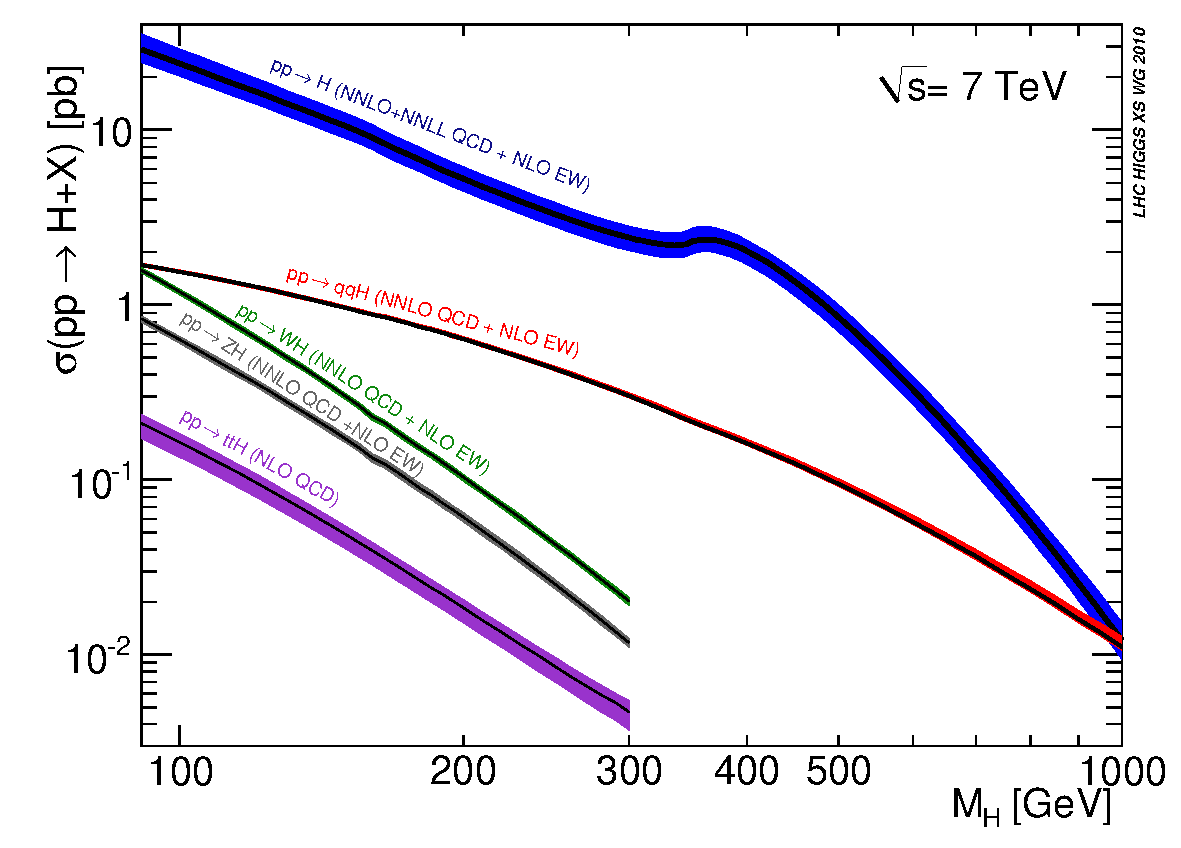
\includegraphics[width=0.54\textwidth]{figs/Higgs_XS_7TeV.pdf}
    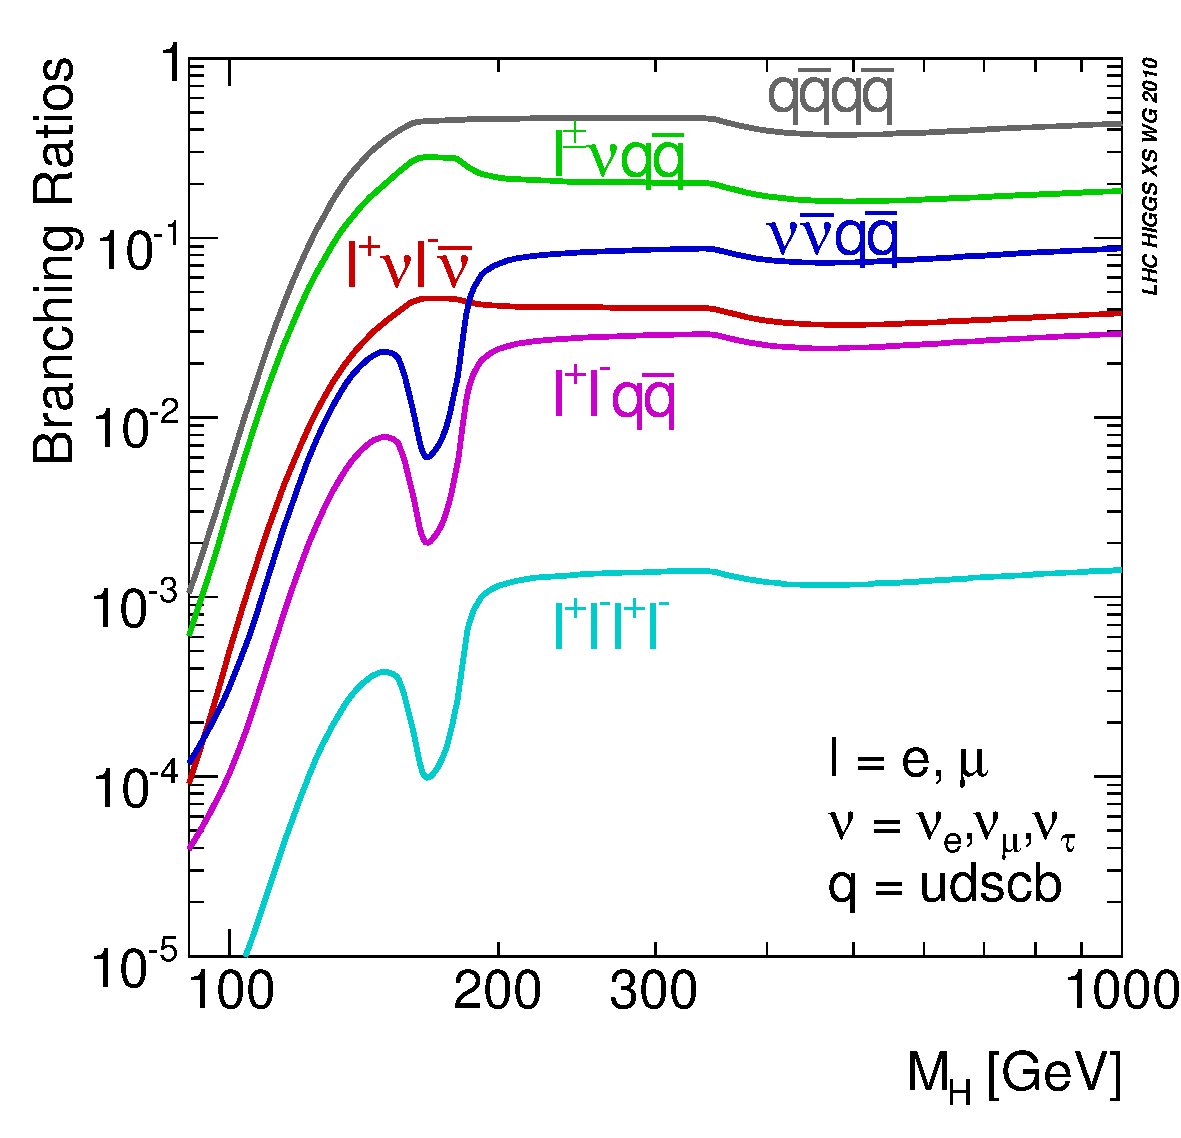
\includegraphics[width=0.42\textwidth]{figs/Higgs_BR_4fermion_1.pdf}
    \caption{Standard Model Higgs boson production cross sections
    (left) and branching ratio into four fermion final states
    (right).}
    \label{fig:higgsXSBR}}
\end{figure}

The expected production cross-section, multiplied by the branching
fraction of the SM Higgs boson decay into a pair of W bosons
\cite{LHCHiggsCrossSectionWorkingGroup:2011ti} and subsequently into a
lepton-neutrino and di-jet pair translates into the effective
cross-section for the analyzed process, as listed in
Table~\ref{tab:signals} as a function of the Higgs mass.

\begin{table}[htb]
  \begin{center}
  \begin{tabular}{c|c|c}
  \hline
  $m_{\textnormal{H}}$ (\GeV)   & $\sigma_{\textnormal{gg}}$ (pb) & $\sigma_{\textnormal{VBF}}$ (pb) \\
  \hline
  300 & $0.48^{+0.08}_{-0.07}$    & $0.060^{+0.003}_{-0.002}$\\
  350 & $0.45^{+0.09}_{-0.07}$    & $0.0416^{+0.002}_{-0.0012}$\\
  400 & $0.34^{+0.05}_{-0.06}$    & $0.0272^{+0.0016}_{-0.0008}$\\
  450 & $0.22^{+0.03}_{-0.04}$    & $0.0197^{+0.0013}_{-0.0006}$\\
  500 & $0.13^{+0.02}_{-0.02}$    & $0.0150^{+0.0011}_{-0.0005}$\\
  550 & $0.084^{+0.016}_{-0.015}$ & $0.0117^{+0.0009}_{-0.0004}$\\
  600 & $0.053^{+0.010}_{-0.010}$ & $0.0093^{+0.0008}_{-0.0004}$\\
  \hline
  \end{tabular}
  \end{center}
  \caption{The cross section for the signal, where the branching fractions of the Higgs into WW
  and of each W into leptons are taken into account in the calculation.}
  \label{tab:signals}
\end{table}%

%%%%%%%%%%%%%%%%%%%%%%%%%%%%%
%%%%%%%%%%%
\subsection {The backgrounds}
%%%%%%%%%%%
All processes yielding one lepton, four jets, 
and missing transverse energy are possible sources 
of background. The most relevant ones are:
%%%%%%%%%%%
\begin{itemize}
  \item W+jets: this is the production of a single W vector boson in
    association with quarks or gluons that mimic the final state
    signature. While the requirement of two additional VBF-tagged jets
    does much to reduce this background, because of its large cross
    section, it is still one of the dominant backgrounds to the
    analysis.
  \item $t\bar{t}$: top quarks pairs are produced at LHC via the gluon
    fusion process $gg\to{}t\bar{t}$ or via QCD quark annihilation
    $q\bar{q}\to{}t\bar{t}$.  The semi-leptonic component, in which
    one W decays hadronically, is reduced by requiring exactly 4 jets
    jets that pass a b-tag veto, while the fully leptonic decay mode
    is reduced by requiring only one good lepton in the event.
    However, because of acceptance and inefficiencies, this background
    still contaminates the signal, and is another dominant background.
  \item Drell-Yan Z/$\gamma^{*}$+jets: this is the production of 
    a single Z/$\gamma^{*}$ boson in association with quarks or gluons, 
    where one lepton escapes undetected because of acceptance or 
    inefficiency effects, and the hadronic activity mimics the final 
    state signature.
  \item WW: this electroweak diboson production is an irreducible 
    background for this analysis. Because its cross-section is measured
    at the LHC, it also serves as a standard candle.
  \item WZ: in case the Z decays hadronically, or the W decays hadronically 
    and one Z lepton is not identified by the detector,
    this sample also contributes to the backgrounds.
  \item ZZ: in case one Z decays hadronically, and one lepton is not identified by the detector,
    this sample contributes to the backgrounds.
  \item Single top production: it proceeds through three separate channels:
    \begin{enumerate}
    \item t-channel: top is produced after a quark-gluon interaction 
      with the exchange of a virtual W.
    \item s-channel: top is produced in association with an anti-bottom, 
      after the annihilation of a pair of quarks in a weak vertex.
    \item tW-channel: top is produced in association with a charged vector boson in a weak process, 
      from a gluon-bottom pair in the initial state.
    \end{enumerate}
  \item QCD multi-jet events generate a background 
       because of the non-negligible probability of jets to be reconstructed as leptons.
\end{itemize}
%%%%%%%%%%%%%%%%%%%%%%
The cross section for the backgrounds, multiplied by the branching ratio when meaningful, 
are reported in Table~\ref{tab:bkg_XS}. 
%%%%%%%%%%%
\begin{table}[htb]
  \begin{center}
  \begin{tabular}{c|c}
  \hline
  Channel & Cross-section (pb) \\
  \hline
  W+jets                        & 31314   \\ %  $\pm$ 1600  \\
  Z+jets                        & 3050    \\ %  $\pm$ 130 \\
  WW                            & 43      \\ %  $\pm$ 1.5 \\
  WZ                            & 18.2    \\ %  $\pm$ 0.7\\
  ZZ                            & 5.90    \\ %  $\pm$ 0.15\\
  t$\bar{\textnormal{t}}$+jets  & 157.5   \\ %  $\pm$ 10 \\
  t+jets ($t$-channel)          & 64.6    \\ % $\pm$ 0.05 \\
  t+jets ($s$-channel)          & 4.6     \\ % $\pm$ 1.1 \\
  t+jets ($t$W-channel)         & 15.7    \\ % $\pm$ 0.8 \\
  QCD (ele enriched)            & 6740000 \\ % $\pm$ \\
  QCD (mu enriched)             & 84700   \\ % $\pm$ \\
  \hline
  \end{tabular}
  \end{center}
  \caption{The cross section for the backgrounds, multiplied by the branching ratio when meaningful.
  Each different sample notation includes all the decays taken into account in the calculation.}
  \label{tab:bkg_XS}
\end{table}%
%
%\begin{table}[htb]
%  \begin{center}
%  \begin{tabular}{c|c}
%  \hline  \hline
%  Channel & Cross-section (pb) \\
%  \hline
%  W+jets                        & 31300   $\pm$ 1600 \\
%  Z+jets                        & 3050    $\pm$  130 \\
%  WW                            & 43.0    $\pm$ 1.5  \\
%  WZ                            & $18.2   $\pm$ 0.7  \\
%  ZZ                            & 5.90    $\pm$ 0.15 \\
%  t$\bar{\textnormal{t}}$+jets  & 157.5   $\pm$   10 \\
%  t+jets ($s$-channel)          & 4.63    $\pm$ 0.19 \\
%  t+jets ($t$-channel)          & 64.57   $\pm$ 2.58 \\
%  t+jets ($t$W-channel)         & 15.74   $\pm$ 1.17 \\
%  QCD (ele enriched)            & 6740000 $\pm$ 100\%\\
%  QCD (mu enriched)             & 84700 $\pm$  100\%\\
%  \hline  \hline
%  \end{tabular}
%  \end{center}
%  \caption{The cross section for the backgrounds, multiplied by the branching ratio when meaningful.}
%  \label{tab:bkg_XS}
%\end{table}%
%%%%%%%%%%%%
%%%%%%%%%%%%%%%%%%%%%%%%%%%%%%%%%%%%%%%%%%%%
\section{Datasets}
\label{sec:technicalities}
% ---- ---- ---- ---- ---- ---- ---- ---- ---- ---- ---- ---- --
\subsection{Data samples}
The data samples used in this analysis were recorded by the CMS experiment in 2010 and 2011.
Only certified runs and luminosity sections are considered, which means that a good functioning
of all CMS sub-detectors is required. The total statistics analyzed correspond to an integrated
luminosity of about $5.0\fbinv$.
% The analysis relies on centrally-produced Primary Datasets (PDs), each of which consists of a collection
% of High Level Trigger (HLT) paths. As explained in Section~\ref{sec:trigger}, single-lepton triggers
% are used to select the events interesting for this analysis in both
% the $e$ and $\mu$ channels, up to an instantaneous luminosity $L \sim 1\cdot10^{33}\percms$. At higher
% luminosities, we move to cross electron+di-jet triggers for the $e$ channel to cope with the
% unsustainable single-electron HLT rate. Therefore, the analysis relies on the so-called ``SingleElectron''
% and ``SingleMu'' PDs for the first data-taking period, and on the ``ElectronHad'' and ``SingleMu'' ones 
% for the most runs. 
The datasets used for the analysis and the corresponding run ranges are listed in Table~\ref{tab:datasets}.
All data samples were reconstructed using a \texttt{CMSSW\_4\_2\_X} release version.
%%%%%%%%%%%
\begin{table}[htb]
  \begin{center}
  \begin{tabular}{r|r}
  \hline  \hline
  Dataset name & Run range \\
  \hline
  /EG/Run2010A-Apr21ReReco-v1/AOD   & 136033 - 144114  \\
  /Mu/Run2010A-Apr21ReReco-v1/AOD   &            \\ 
  \hline
  /Electron/Run2010B-Apr21ReReco-v1/AOD   &  144919 - 149442  \\
  /Mu/Run2010B-Apr21ReReco-v1/AOD         &             \\
  \hline
  /SingleElectron/Run2011A-May10ReReco-v1/AOD   & 160431 - 163869 \\
  /SingleMu/Run2011A-May10ReReco-v1/AOD         &                 \\
  \hline                                     
  /SingleElectron/Run2011A-PromptReco-v4/AOD       & 165088 - 167913   \\
  /SingleMu/Run2011A-PromptReco-v4/AOD          &                 \\
  \hline                                     
  /SingleElectron/Run2011A-05Aug2011-v1/AOD        & 170826 - 172619 \\
  /SingleMu/Run2011A-05Aug2011-v1/AOD           &                 \\
  \hline                                     
  /SingleElectron/Run2011A-PromptReco-v6/AOD       & 172620 - 173692 \\
  /SingleMu/Run2011A-PromptReco-v6/AOD          &                 \\
  \hline                                     
  /SingleElectron/Run2011B-PromptReco-v1/AOD       & 175832 - 180252 \\
 /SingleMu/Run2011B-PromptReco-v1/AOD          &                 \\
  \hline  \hline
  \end{tabular}
  \end{center}
  \caption{Summary of the data samples used and the run ranges of applicability.}
  \label{tab:datasets}
\end{table}%
%%%%%%%%%%%
%%%%%%%%%%%%%%%%%%%%%%%%%%%%%%%%%%%%%%%%%%%%
\subsection{Monte Carlo samples}
Standard Model Higgs boson samples, 
as well as samples for a large variety of electroweak and QCD-induced background sources, 
have been generated and showered using different Monte Carlo generators.
To better reproduce the actual data-taking conditions, where there is a significant probability
that more than two protons interact in the same bunch crossing, pile-up (PU) events are
added on top of the hard scattering. Particle interactions with the detector were reproduced through
a detailed description of CMS.

The POWHEG-BOX generator \cite{Nason:2004rx,Frixione:2007vw,Alioli:2010xd,Nason:2009ai} has been used to
produce Higgs signal events, and the showering has been performed with PYTHIA6 \cite{pythia}. For this analysis, 
samples with Higgs mass hypotheses ranging from 300 to 600\GeV have been used.
 

The background and signal samples used for the studies are listed in Table~\ref{tab:MCsamples},
together with the equivalent luminosity available for the study.
All background MC samples considered in this analysis come from 
the official ``Fall11'' production. Events were
reconstructed making use of a \texttt{CMSSW\_4\_2\_X} release version. 
% The pile-up scenario used for
% these samples consists of a flat distribution of PU events up to ten additional interactions on top
% of the hard scattering plus a poissonian tail with a mean of ten interactions; only pile-up occurring 
% in the same bunch crossing of the main event (in time PU) was considered.
%%%%%%%%%%%%%%%%%%%%%%%%%%%%%%%%%
\begin{sidewaystable}[htb]
  \begin{center}
    \begin{tabular}{l} 
      \hline\hline
      sample \\
      \hline
      /W4Jets\_TuneZ2\_7TeV-madgraph-tauola/Fall11-PU\_S6\_START42\_V14B-v1/AODSIM \\
%%    /WJetsToLNu\_TuneZ2\_7TeV-madgraph-tauola/Fall11-PU\_S6\_START42\_V14B-v1/AODSIM    \\
      /WW\_TuneZ2\_7TeV\_pythia6\_tauola/Fall11-PU\_S6\_START42\_V14B-v1/AODSIM     \\
      /WZ\_TuneZ2\_7TeV\_pythia6\_tauola/Fall11-PU\_S6\_START42\_V14B-v1/AODSIM     \\
      /TTJets\_TuneZ2\_7TeV-madgraph-tauola/Fall11-PU\_S6\_START42\_V14B-v2/AODSIM    \\
      /QCD\_Pt-20\_MuEnrichedPt-15\_TuneZ2\_7TeV-pythia6/Fall11-PU\_S6\_START42\_V14B-v2/AODSIM  \\      
      /DYJetsToLL\_TuneZ2\_M-50\_7TeV-madgraph-tauola/Fall11-PU\_S6\_START42\_V14B-v1/AODSIM   \\
      /Tbar\_TuneZ2\_s-channel\_7TeV-powheg-tauola/Fall11-PU\_S6\_START42\_V14B-v1/AODSIM     \\
      /Tbar\_TuneZ2\_t-channel\_7TeV-powheg-tauola/Fall11-PU\_S6\_START42\_V14B-v1/AODSIM     \\
      /Tbar\_TuneZ2\_tW-channel-DS\_7TeV-powheg-tauola/Fall11-PU\_S6\_START42\_V14B-v1/AODSIM    \\
      /T\_TuneZ2\_s-channel\_7TeV-powheg-tauola/Fall11-PU\_S6\_START42\_V14B-v1/AODSIM     \\
      /T\_TuneZ2\_t-channel\_7TeV-powheg-tauola/Fall11-PU\_S6\_START42\_V14B-v1/AODSIM     \\
      /T\_TuneZ2\_tW-channel-DS\_7TeV-powheg-tauola/Fall11-PU\_S6\_START42\_V14B-v1/AODSIM     \\
      \hline
      /WJetsToLNu\_TuneZ2\_matchingdown\_7TeV-madgraph-tauola/Summer11-PU\_S4\_START42\_V11-v1/AODSIM  \\
      /WJetsToLNu\_TuneZ2\_matchingup\_7TeV-madgraph-tauola/Summer11-PU\_S4\_START42\_V11-v1/AODSIM  \\
      /WJetsToLNu\_TuneZ2\_scaledown\_7TeV-madgraph-tauola/Summer11-PU\_S4\_START42\_V11-v1/AODSIM          \\
      /WJetsToLNu\_TuneZ2\_scaleup\_7TeV-madgraph-tauola/Summer11-PU\_S4\_START42\_V11-v1/AODSIM            \\
      /WToLNu\_1jEnh2\_2jEnh35\_3jEnh40\_4jEnh50\_7TeV-sherpa/Summer11-PU\_S4\_START42\_V11-v1/AODSIM      \\
      \hline 
      /GluGluToHToWWToLNuQQ\_M-*\_7TeV-powheg-pythia6/Fall11-PU\_S6\_START42\_V14B-v1/AODSIM  \\
      /VBF\_HToWWToLNuQQ\_M-*\_7TeV-powheg-pythia6/Fall11-PU\_S6\_START42\_V14B-v1/AODSIM \\
      Higgs mass from 300 to 600~GeV   \\
      \hline\hline
    \end{tabular}
  \end{center}
  \caption{Summary of Monte Carlo samples used in the analysis for background and signal modeling and for systematic studies.}
  \label{tab:datasets:mcstat}
  %FIXME add the corresponding cross-sections
  \label{tab:MCsamples}
\end{sidewaystable}
%%%%%%%%%%%%%%%%%%%%%%%%%%%%%%%%%
\clearpage
%%%%%%%%%%%%%%%%%%%%%%%%%%%%%%%%%%%%%%%%%%%%%%%%%%
%%%%%%%%%%%%%%%%%%%%%%%%%%%%%%%%%%%%%%%%%%%%%%%%%%
%%%%%%%%%%%%%%%%%%%%%%%%%%%%%%%%%%%%%%%%%%%%%%%%%%
%%%%%%%%%%%%%%%%%%%%%%%%%%%%%%%%%%%%%%%%%%%%%%%%%%
\section{Physics objects reconstruction}
\label{sec:reco}
\label{sec:firstStep}
% ---- ---- ---- ---- ---- ---- ---- ---- ---- ---- ---- ---- ---- ---- ----
The event reconstruction and selection criteria are described in
detail in \cite{CMS-AN-2011-110}, Section 4.  The lepton requirements
are identical, whereas the addition of two VBF-tagged jets requires a
change in the jet sector. Here we summarize the selection requirements
in brief.

%%%%%%%%%%%%%%%%%%%%%%%%%%%%
\subsection{Electron selection}
\label{sec:electron_cuts}

%%%%%%%%%%%%%%%%%%%
\begin{itemize}
\item Electron cut-based electron ID requiring 'VBTF Working Point 70'.
\item Electron $E_\mathrm{T} > 35\,\mathrm{GeV}$.
\item Pseudorapidity $|\eta| < 2.5$. There is an exclusion range due
        to the ECAL barrel-endcap transition region, defined by
        $1.4442 < |\eta_{\mathrm{sc}}| < 1.566$, where
        $\eta_{\mathrm{sc}}$ is the pseudorapidity of the ECAL
        supercluster.
\item Impact parameter: We cut on the absolute value of the impact
       parameter calculated with respect to the average beamspot. We
       require:  $d_0(\mathrm{Bsp}) < 0.02\,\mathrm{cm}.$   
\item The selected electron candidates have to be isolated simultaneously in
the tracker, and in the electromagnetic and hadronic calorimeters.  Combined
relative isolation is defined as
%%%
\begin{equation*}
\mathrm{RelIso_{\mathrm{Comb}}} = \frac{I_{\mathrm{Trk}}+I_{\mathrm{EM}}+I_{\mathrm{had}}}{E_\mathrm{T}}.
\end{equation*} 
%%%
The electron candidate is required to have 
$\mathrm{RelIso_{\mathrm{Comb}}} < 0.05$ in order 
to be considered isolated. 
A pile-up offset subtraction in the isolation cone 
using fastjet algorithm \cite{FastJetPUSubtraction} is applied.
\item
We also veto the presence of a second loose lepton in the event.
\item 
Electron-to-photon conversion rejection: we
require the number of missed inner tracker layers of the electron
track to be exactly zero and reject electrons with
distance of the partner track $|$\texttt{dist}$|$ $< 0.02$~mm and an
opening angle $|$\texttt{dcot}$|$ $< 0.02$~\cite{ConversionRejection}.
\end{itemize}
%%%%%%%%%%%%%%%%%%%
%%%%%%%%%%%%%%%%%%%
%%%%%%%%%%%%%%%%%%%%%%%%%%%%%%%%%%%%%%%%%%%%%%%%%%%%%%%%%%%%%%%%%%%%%%%%%%%%
%%%%%%%%%%%%%%%%%%%%%%%%%%%%%%%%%%%%%%%%%%%%%%%%%%%%%%%%%%%%%%%%%%%%%%%%%%%%
\subsection{Muon selection}
\label{sec:muon_cuts}
%%%%%%%%%%%%%%%%%%%
\begin{itemize}
\item The muon candidate is reconstructed both as a global muon and
as a tracker muon~\cite{MUONPAS}.
\item The number of hits of the muon track in the silicon tracker has
to be $N_{\mathrm{Hits}} > 10$.
\item Number of pixel hits of the Tracker track $\ge 1$;
\item Number of muon hits of the Global track $\ge 2$;
\item Normalized $\chi^{2}$ of the Global track $< 10.0$.
\item Muon $p_{\mathrm{T}} > 25\,\mathrm{GeV}$.
\item Pseudorapidity $|\eta| < 2.1$.
\item Impact parameter: We cut on the absolute value of the impact
parameter calculated with respect to the beamspot. We require:
$d_0(\mathrm{Bsp}) < 0.02\,\mathrm{cm}.$
\item In order to make sure that the selected muon and the selected
jets come from the same hard interaction and not from pile up events,
we require that the $z$ coordinate of the PV of the event and the $z$
coordinate of the muon's inner track vertex lie within a distance of
less than 1~cm.
\item The selected muon candidates also have to be isolated.
We require the muon to be isolated simultaneously in the
tracker, and in the electromagnetic and hadronic calorimeters.  
The muon candidate is required to have
$\mathrm{RelIso_{\mathrm{Comb}}} < 0.1$ in order to be considered
isolated.
We also veto the presence of a second loose lepton in the event.
\end{itemize}
%%%%%%%%%%%%%%%%%%%%%%%%%%%%
%%%%%%%%%%%%%%%%%%%%%%%%%%%%
%%%%%%%%%%%%%%%%%%%%%%%%%%%%%%%%%%%%%%%%%%%%%%%%%%%%%%%%%%%%%%%%%%%%%%%%%%%%
%%%%%%%%%%%%%%%%%%%%%%%%%%%%%%%%%%%%%%%%%%%%%%%%%%%%%%%%%%%%%%%%%%%%%%%%%%%%

\subsection{Loose Electron}
For the purposes of rejecting events with more than one lepton we
define a loose electron, which has looser cuts. We consider electrons
which have $p_{\mathrm{T}} > 15\,\mathrm{GeV}/c$, $|\eta| < 2.5$, and
$\mathrm{RelIso_{\mathrm{Trk}}} < 0.2$ and which satisfy electron ID
cuts according to ``VBTF Working Point 95'' to be ``loose''. The cut
values for the electron ID variables used in the analysis can be found
in \cite{CMS-AN-2011-110} Table~6.

\subsection{Loose Muon}
Additionally, to reject events with more than one lepton, we define a
loose muon, which has looser cuts. We consider all global muons which
have $p_{\mathrm{T}} > 10\,\mathrm{GeV}/c$, $|\eta| < 2.5$, and
$\mathrm{RelIso_{\mathrm{Trk}}} < 0.2$ to be loose muons.

\subsection{Jet selection}
\label{sec:firstStep_jets}
Jets are reconstructed exactly as defined in \cite{CMS-AN-2011-110}.
In this analysis we use jets with measured (corrected) $\PT$  
greater than 30~$\gev$. 

We first require that two VBF-tagged jets exist in the event, for which
\begin{itemize}
\item $|\eta_{j}| < 4.5$
\item $\eta_{j1} \times \eta_{j2} < 0$
\item $|\eta_{j1} - \eta_{j2}| > 3.5$
\item $m_{j1j2} > 300$~GeV.
\end{itemize}

If more than two possible jet pairs are found that meet these criteria,
the pair with the maximum $|\Delta\eta|$ is taken.

After choosing the tagged jets, we subsequently require two central
jets  $|\eta| < 2.4$ with the largest $p_T$ (both exceeding 30~GeV)
to comprise the hadronic W.
Jets are required to pass a set of loose identification
criteria; this requirement eliminates jets originating from or being seeded by
noisy channels in the calorimeter~\cite{Chatrchyan:2009hy}: 
%%%%%%%%%%%%%%
\begin{itemize}
\item Fraction of energy due to neutral hadrons $<$ 0.99.
\item Fraction of energy due to neutral EM deposits $<$ 0.99.
\item Number of constituents $>$ 1.
\item Number of charged hadrons candidates $>$ 0.
\item Fraction of energy due to charged hadrons candidates $>$ 0.
\item Fraction of energy due to charged EM deposits $<$ 0.99.
\end{itemize}
%%%%%%%%%%
All energy fractions are calculated from uncorrected jets.

\par
In order to account for electron and muon objects that
have been reconstructed as jets, we remove from the jet
collection any jet that falls within a
cone of radius $R= 0.3$ of a loose electron or a loose muon. 
This ``cleaning'' procedure is applied in order to ensure that the same
particle is not double counted as two different physics objects.

Finally, since $\ttbar$ becomes a more significant background for
the VBF channel, we require that all four jets are required to pass a
b-tag veto. The algorithm used to determine the jet b-tagging is
the Simple Secondary Vertex High Efficiency (SSVHE) algorithm \cite{btag}.

%%%%%%%%%%%%%%%%%%%%%%%%%%%%%%%%%%%%%%%%%%%%%%%%%%%%%%
%%%%%%%%%%%%%%%%%%%%%%%%%%%%%%%%%%%%%%%%%%%%%%%%%%%%%%
\subsection{Missing transverse energy requirement}
\label{sec:MET}
An accurate MET measurement is essential for distinguishing
the $\Wo$ signal from QCD backgrounds. 
We use the MET estimate provided by the Particle Flow algorithm.
PF MET showed the best performance
among several MET algorithms~\cite{PFMET}.
The MET is computed as the vector sum of all PF objects.
A good agreement is found between the MET
distributions of $\Wln$ events in data and simulation~\cite{metPAS}.
The resolution for inclusive multi-jet samples and for
$\Wln$ events is also well reproduced by the simulation.  
A relative broadening of a few percent is observed in the data compared to MC,  
and has a negligible impact on the
extraction of the W yields~\cite{WZCMS:2010}.

We require the event to have missing transverse energy
MET in excess of 25~GeV in case of muon sample and 
30 GeV in case of electron sample.
We also require W transverse mass $ > 50\,\mathrm{GeV}$.
These cuts are designed to reduce the background
from QCD multijet production.
%%%%%%%%%%%%%%%%%%%%%%%%%%%%%%%%%%%%%%%%%%%%%%%%%%%%%%
%%%%%%%%%%%%%%%%%%%%%%%%%%%%%%%%%%%%%%%%%%%%%%%%%%%%%%
%%%%%%%%%%%%%%%%%%%%%%%%%%%%%%%%%%%%%%
%%%%%%%%%%%%%%%%%%%%%%%%%%%%%%%%%%%%%%
%%%%%%%%%%%%%%%%%%%%%%%%%%%%%%%%%%%%%%%%%%%%%%%%%%%%%%%%%%%%%%%%%%%%
%%%%%%%%%%%%%%%%%%%%%%%%%%%%%%%%%%%%%%%%%%%%%%%%%%%%%%%%%%%%%%%%%%%%
%%%%%%%%%%%%%%%%%%%%%%%%%%%%%%%%%%%%%%%%%%%%%%%%%%%%%%%%%%%%%%%%%%%%
\section{Lepton reconstruction and selection efficiency}
\label{sec:efficiency}
The lepton efficiency and data/MC scale factors computed using 
the ``tag \& probe'' technique are described in detail in the CMS analysis note 
AN-2012/021.
%%%%%%%%%%%%%%%%%%%%%%%%%%%%%%%%%%%%%%%%%%%%%%%%%%%%%%%%%%%%%%%%%%%%
%%%%%%%%%%%%%%%%%%%%%%%%%%%%%%%%%%%%%%%%%%%%%%%%%%%%%%%%%%%%%%%%%%%%
%%%%%%%%%%%%%%%%%%%%%%%%%%%%%%%%%%%%%%%%%%%%%%%%%%%%%%%%%%%%%%%%%%%%
\section{Trigger selection and efficiency}
\label{sec:trigger}
The trigger selection used in this analysis and the trigger efficiency 
computation are also described in detail in the CMS analysis note 
AN-2012/021.
%%%%%%%%%%%%%%%%%%%%%%%%%%%%%%%
%%%%%%%%%%%%%%%%%%%%%%%%%%%%%%%

\section{Comparison of Data and Monte Carlo simulation}
To assess the quality of the modeling provided by the MC simulation we 
make comparisons between the MC shape normalized to the total
prediction for the background compared to the overall data
yield after applying the event selection criteria. 
We show the distributions of various kinematic
variables after applying all the selection cuts in 
Figures ~\ref{fig:mu_wjet_pt}-\ref{fig:mu_tagjet_pair}
for the muon+jets sample and in 
Figures ~\ref{fig:el_jet_pt}-\ref{fig:el_tagjet_pair} for
the electron+jets sample. The MC has been been corrected for
lepton reconstruction and selection efficiency and the trigger efficiency.
Seeing reasonable agreement gives us confidence in
the qualitative aspects of the MC modeling. 
%%%%%%%%%%%%%%%%%%%%%%%%%%%%
\begin{figure}[ht]
  {\centering
    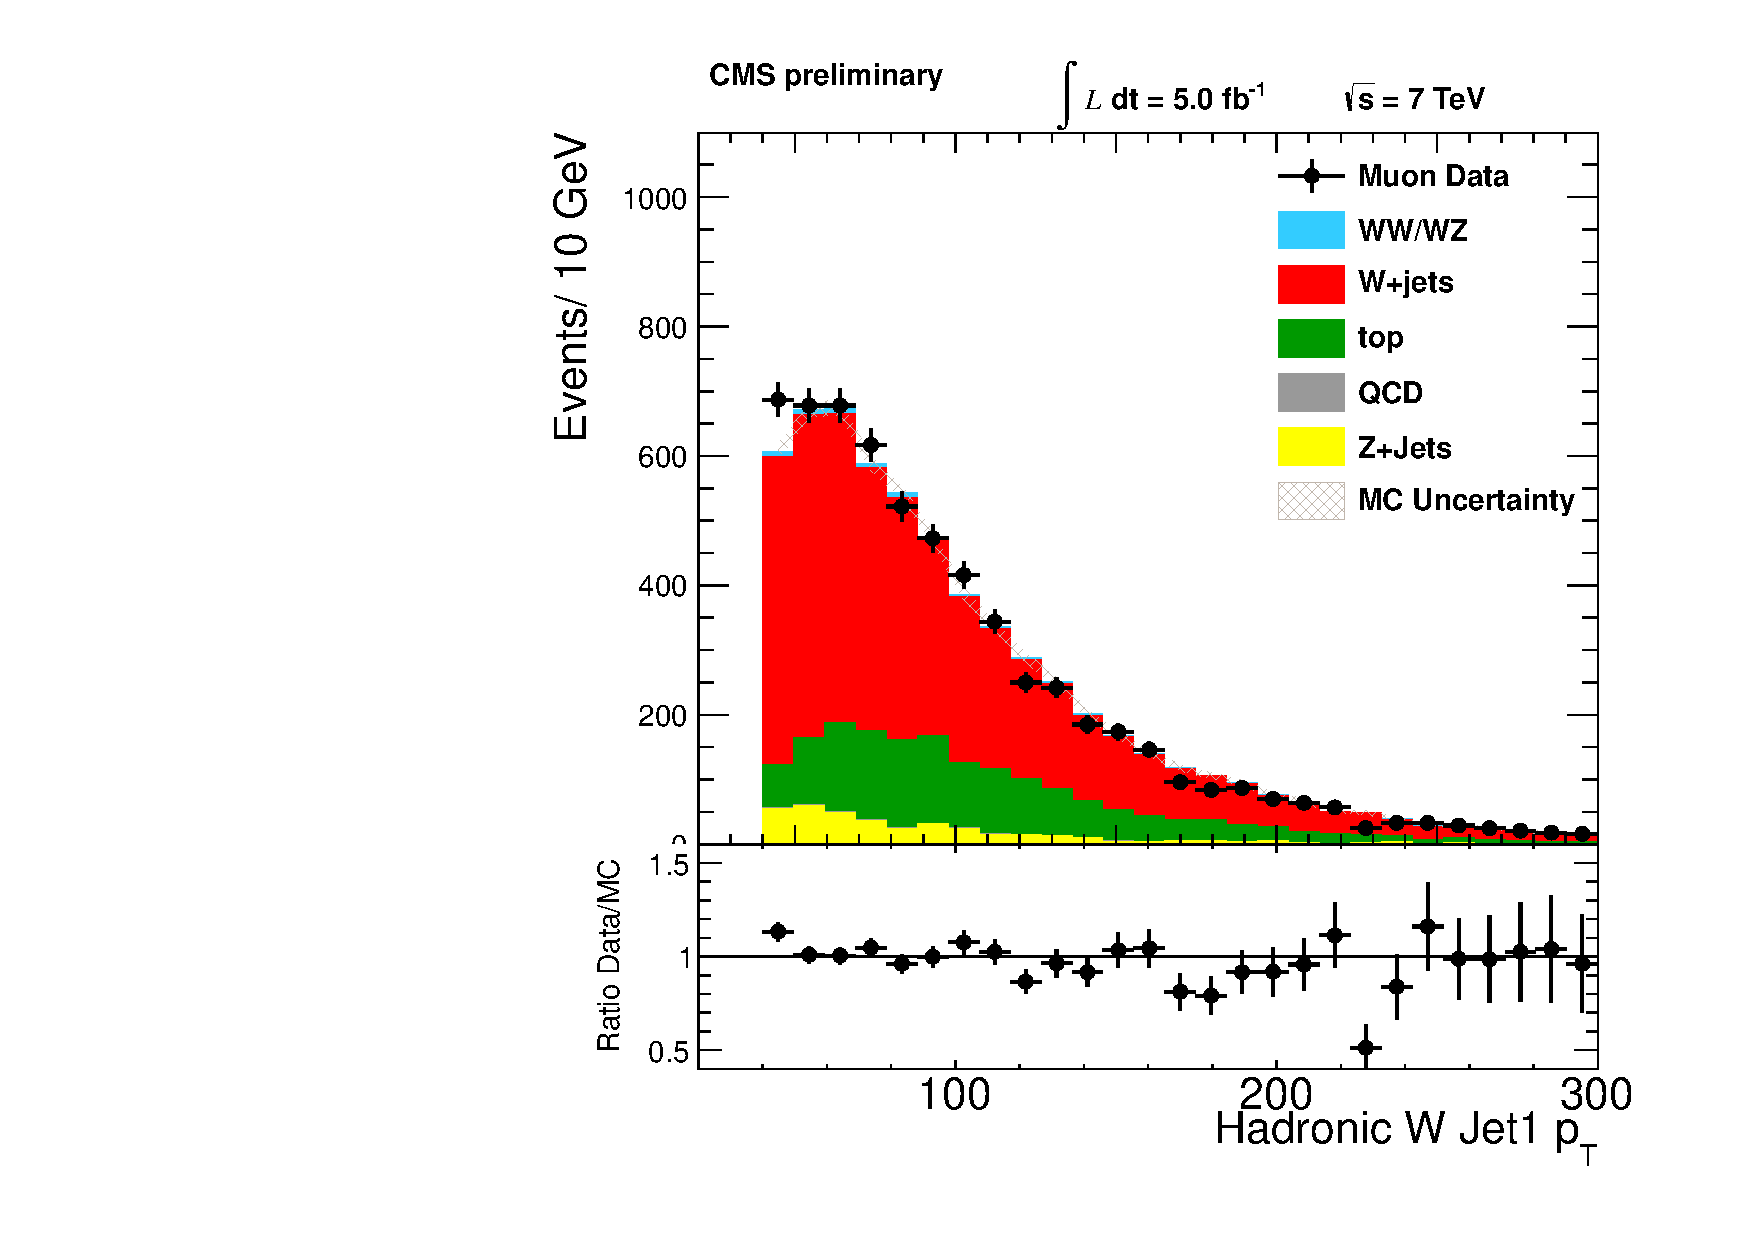
\includegraphics[width=0.49\textwidth]{figs/n-1_plots_mu/mu_vbfwjeta_pt.pdf}
    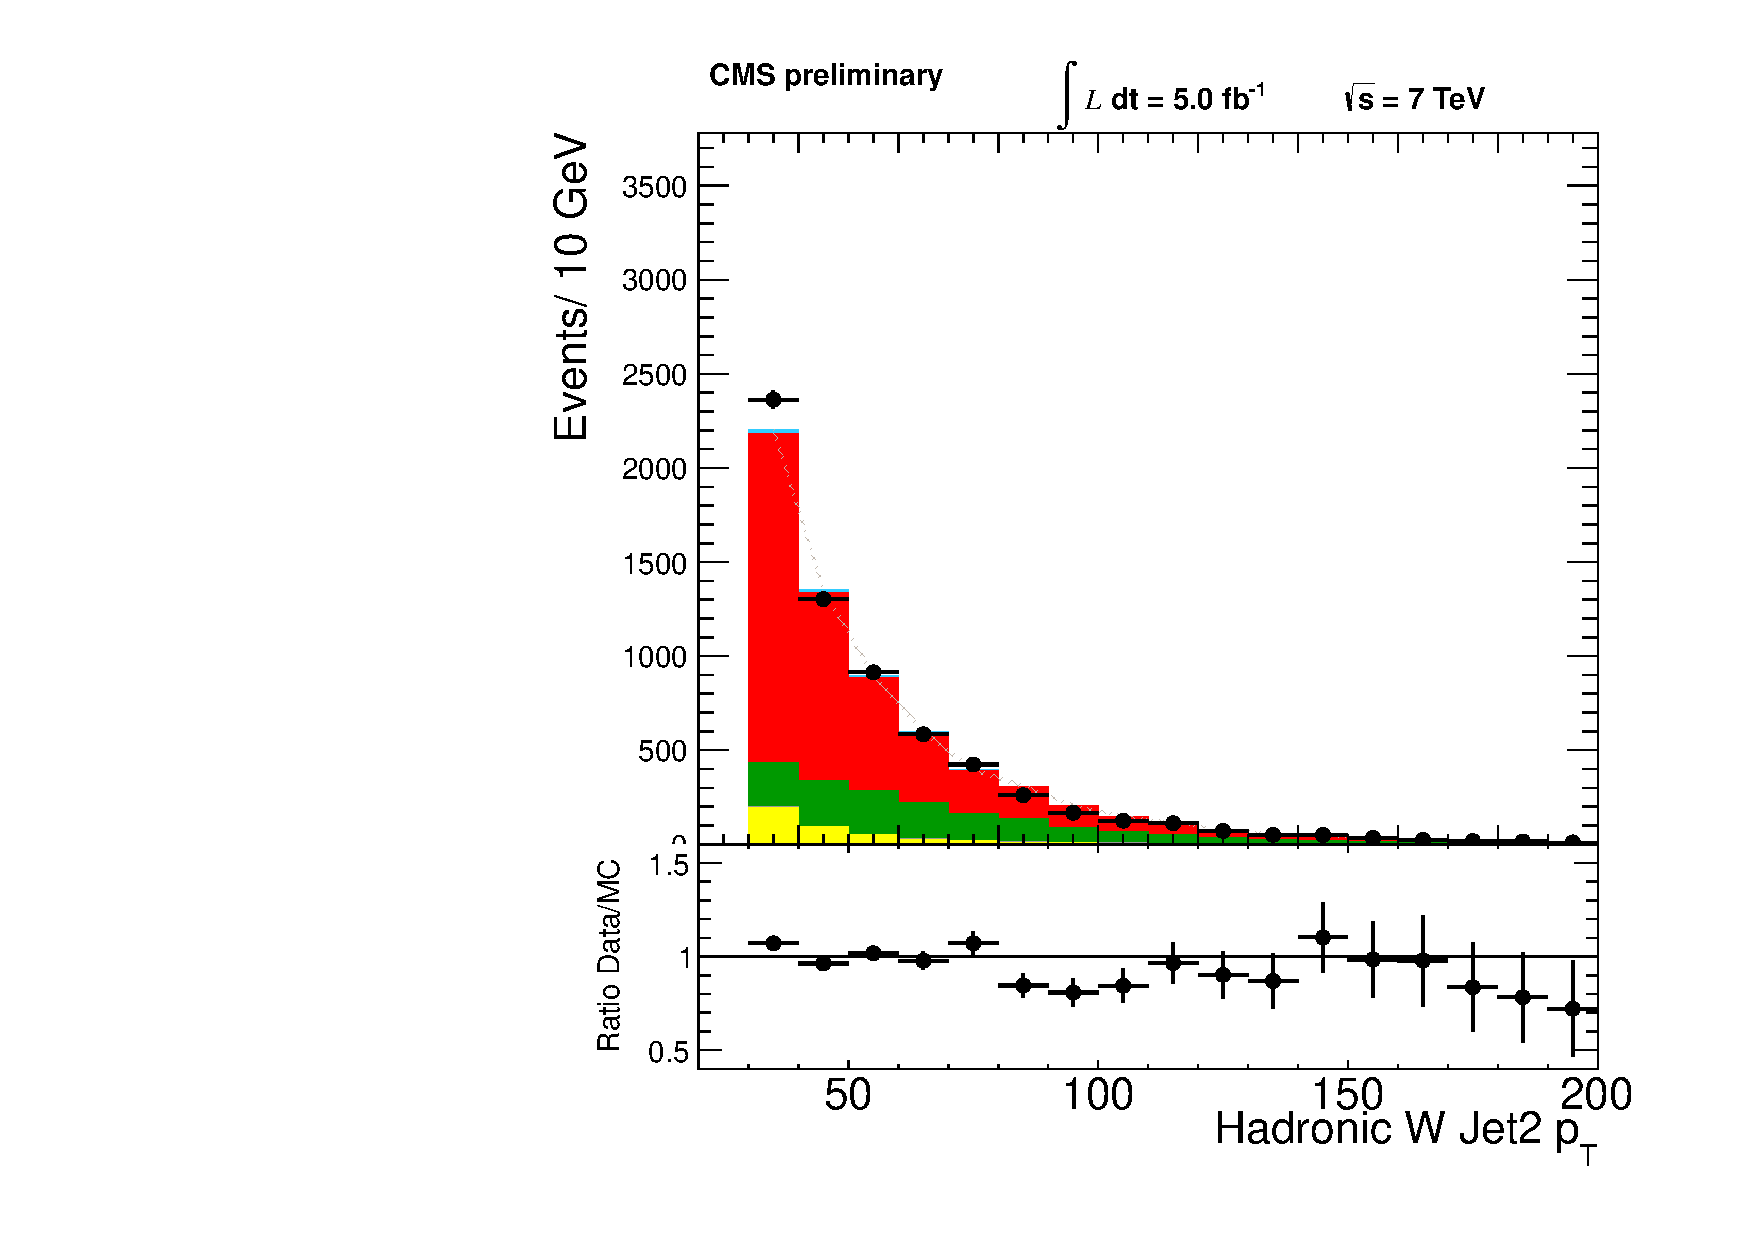
\includegraphics[width=0.49\textwidth]{figs/n-1_plots_mu/mu_vbfwjetb_pt.pdf}
    \caption{Comparison of the first (left) and second (right)
      hadronic W jet $p_{T}$ distributions from data and MC for the
      muon+jets selection.}
    \label{fig:mu_wjet_pt}}
\end{figure}
%%%%%%%%%%%%%%%%%%%%%%%%%%%%
\begin{figure}[h!t]
  {\centering
    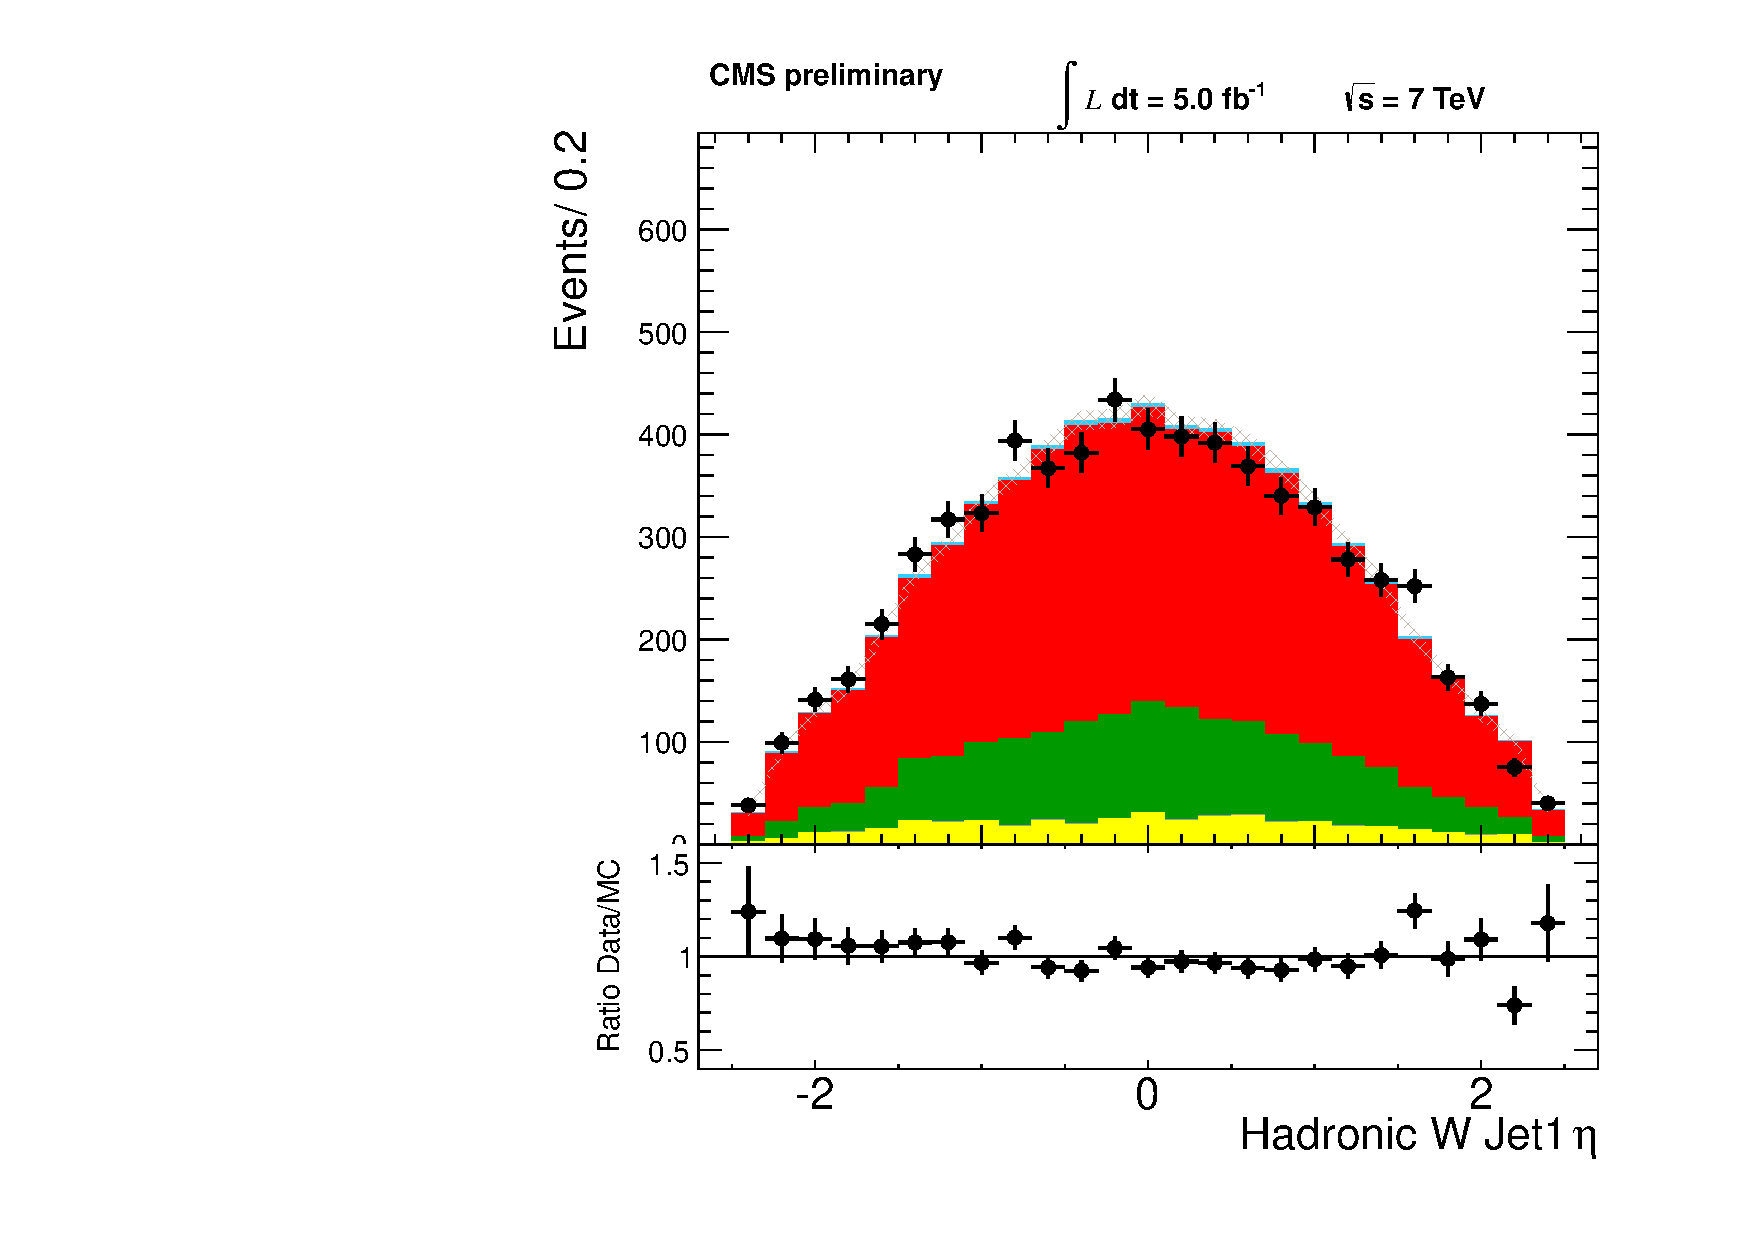
\includegraphics[width=0.49\textwidth]{figs/n-1_plots_mu/mu_vbfwjeta_eta.pdf}
    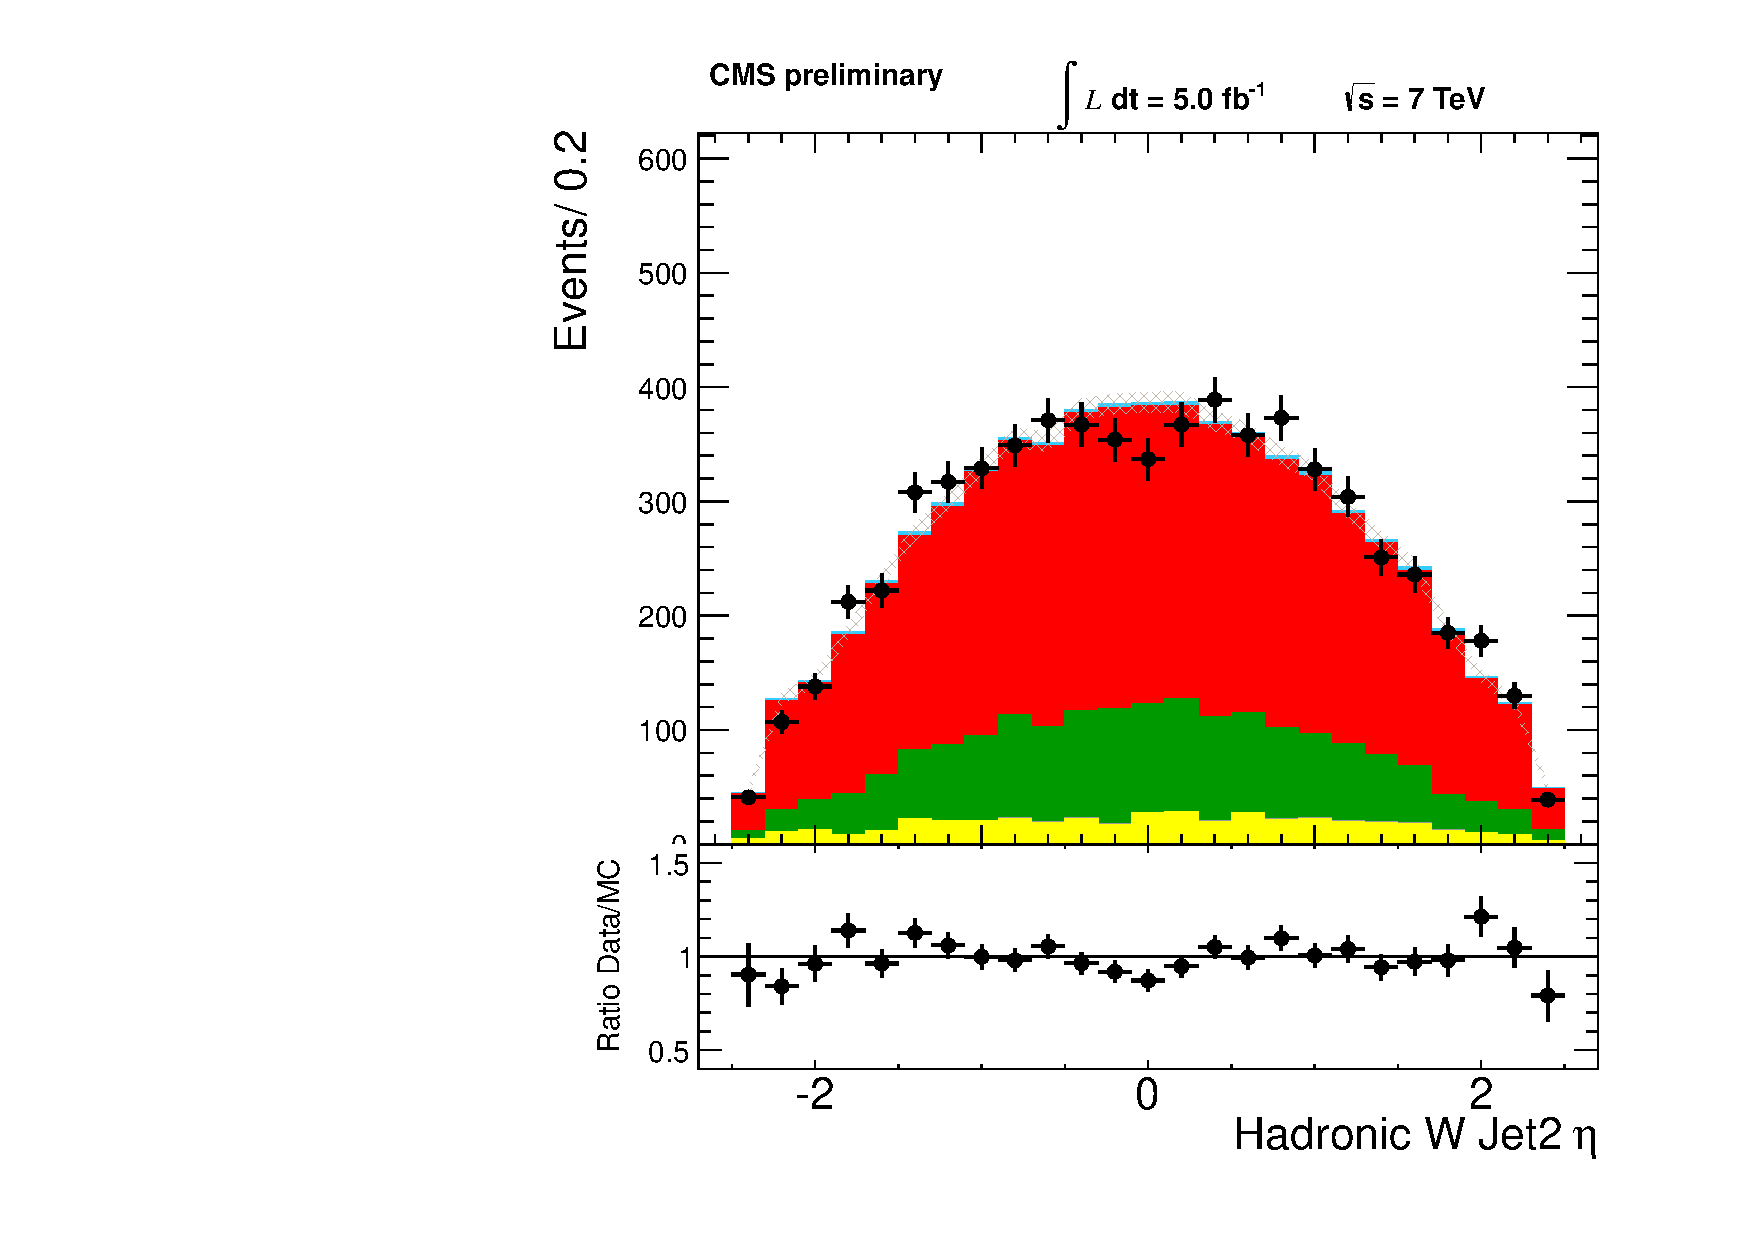
\includegraphics[width=0.49\textwidth]{figs/n-1_plots_mu/mu_vbfwjetb_eta.pdf}
    \caption{Comparison of the first (left) and second (right)
    hadronic W jet $\eta $ distributions from data and MC for the
    muon+jets selection.  }
\label{fig:mu_wjet_eta}}
\end{figure}

%%%%%%%%%%%%%%%%%%%%%%%%%%%%
\begin{figure}[h!t]
  {\centering
    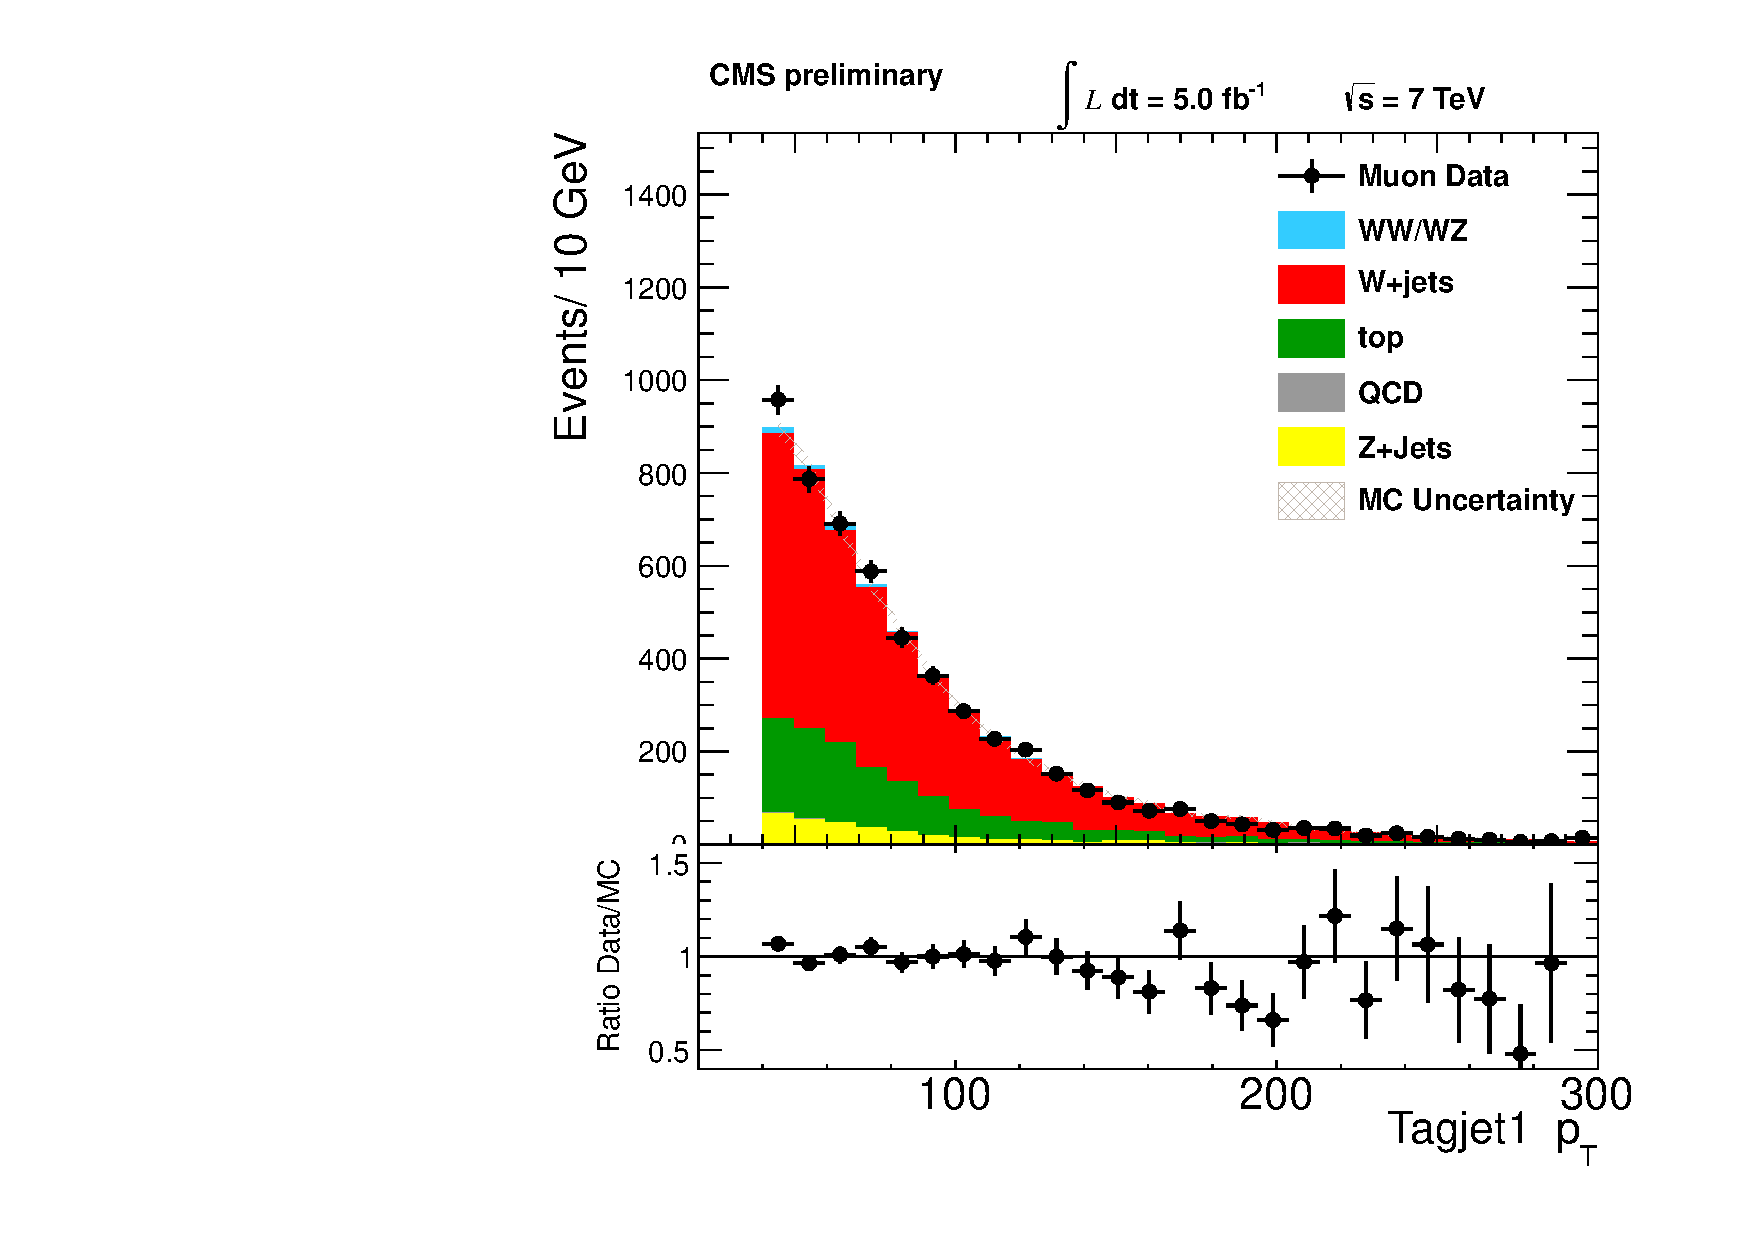
\includegraphics[width=0.49\textwidth]{figs/n-1_plots_mu/mu_vbftagjeta_pt.pdf}
    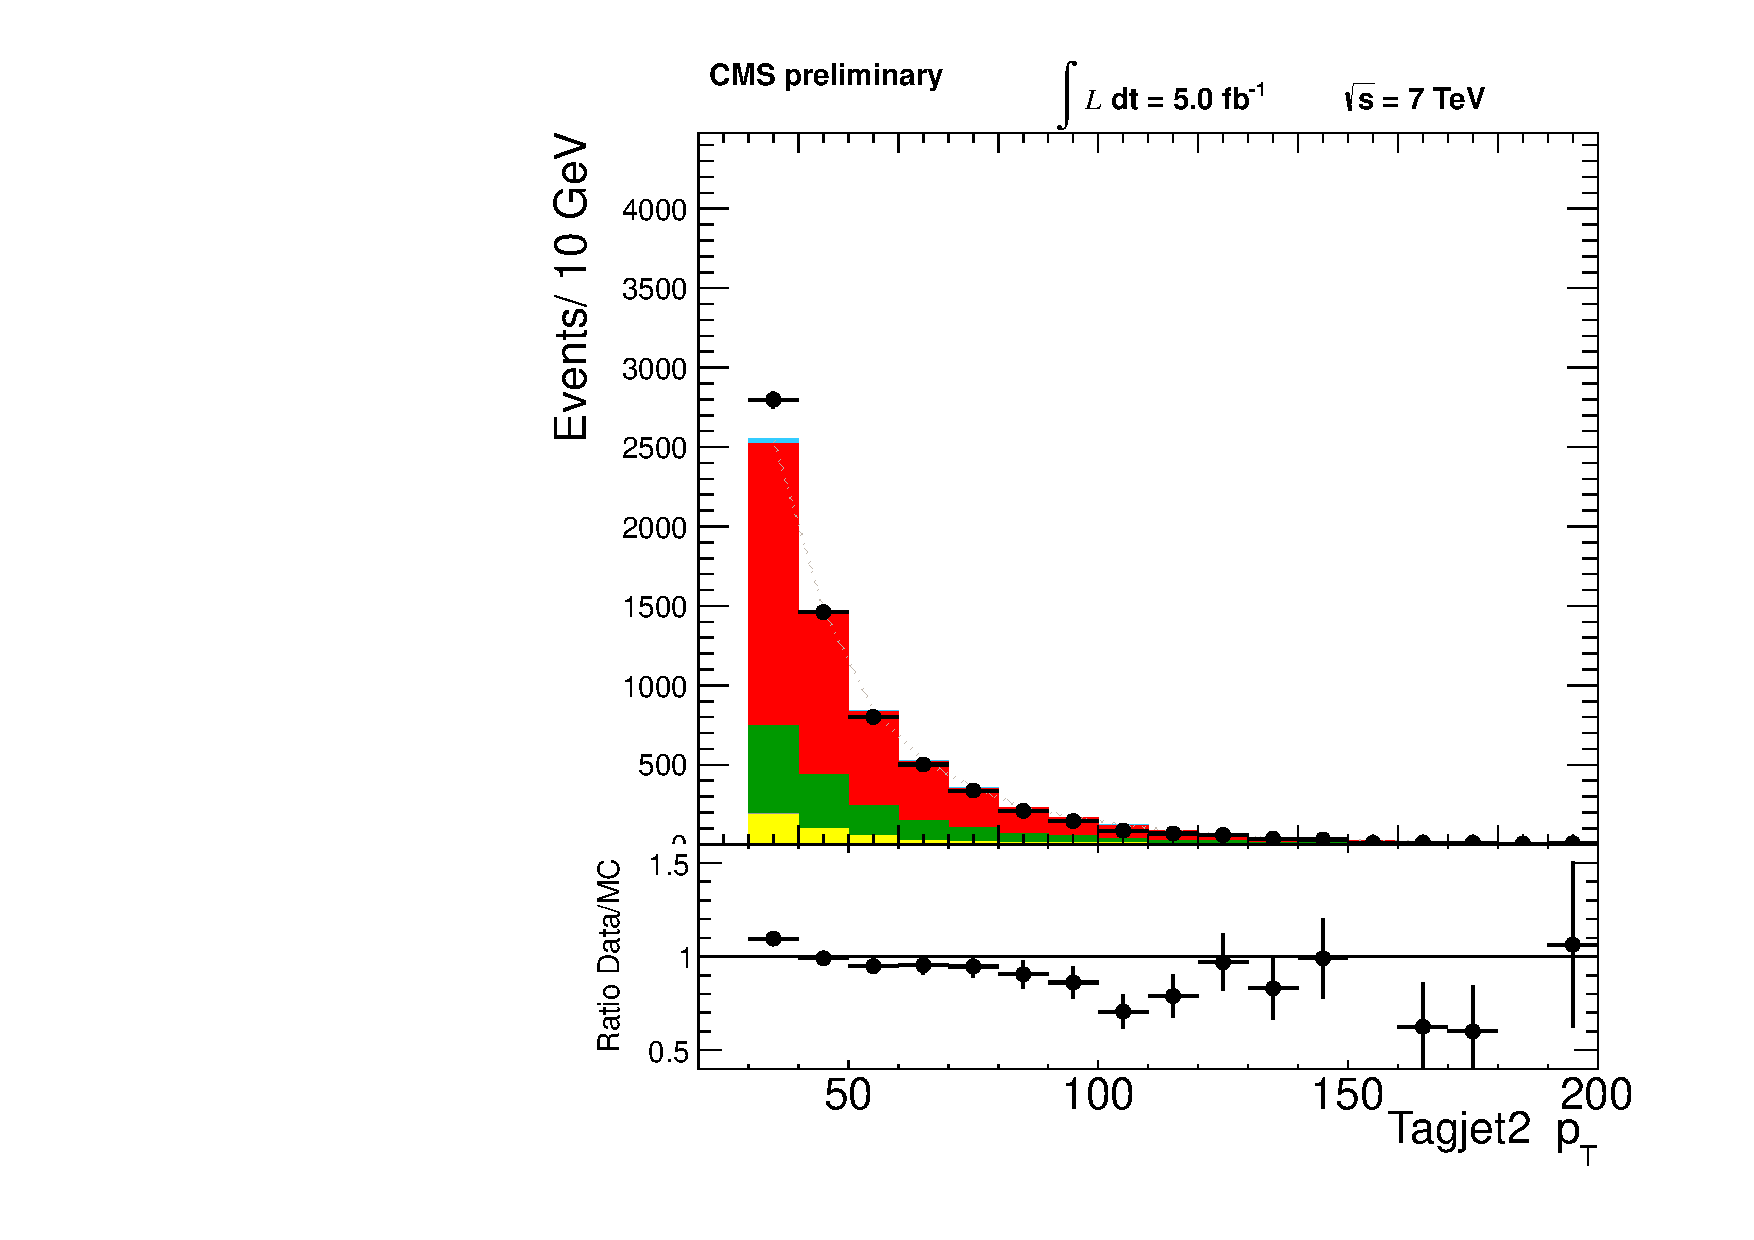
\includegraphics[width=0.49\textwidth]{figs/n-1_plots_mu/mu_vbftagjetb_pt.pdf}
    \caption{Comparison of the first (left) and second (right)
      VBF-tagged jet $p_{T}$ distributions from data and MC for the
      muon+jets selection.}
    \label{fig:mu_tagjet_pt}}
\end{figure}

%%%%%%%%%%%%%%%%%%%%%%%%%%%%
\begin{figure}[h!t]
  {\centering
    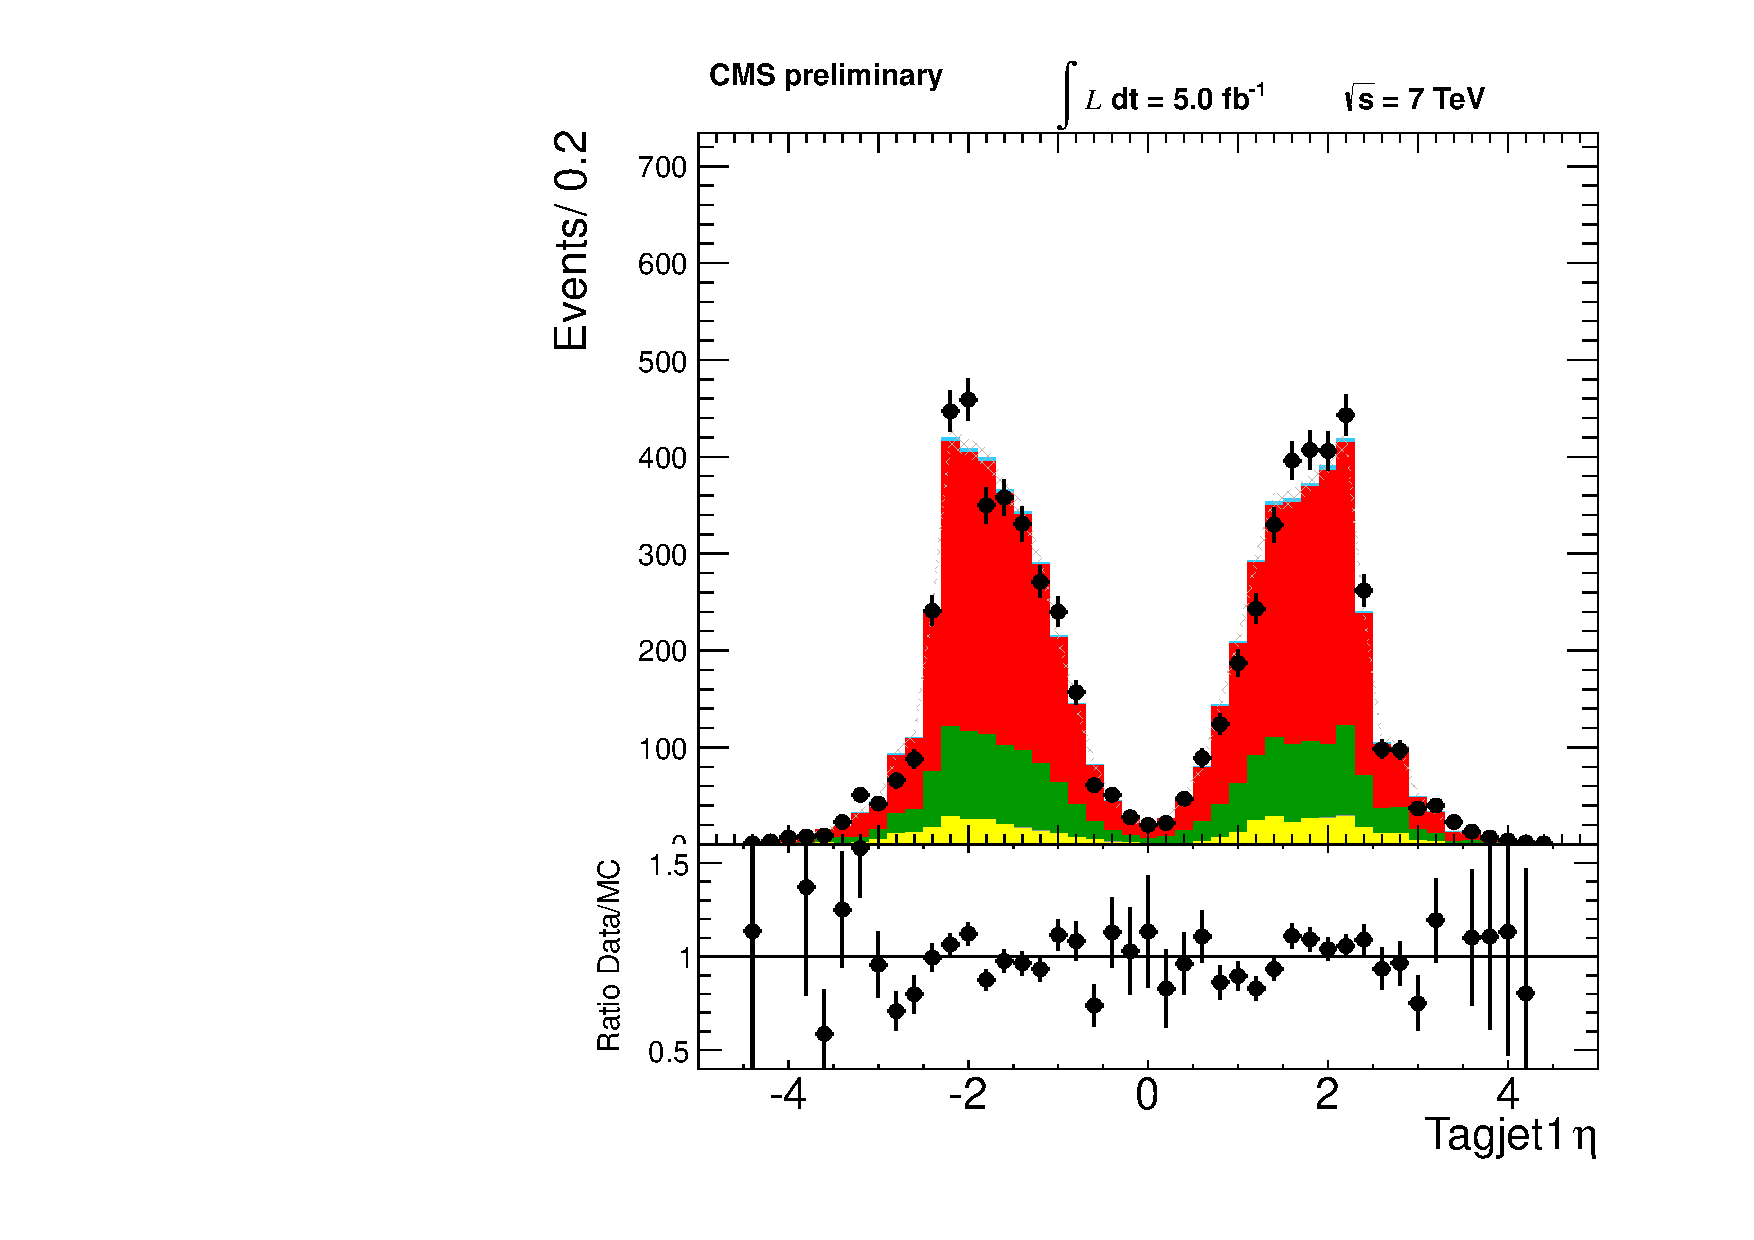
\includegraphics[width=0.49\textwidth]{figs/n-1_plots_mu/mu_vbftagjeta_eta.pdf}
    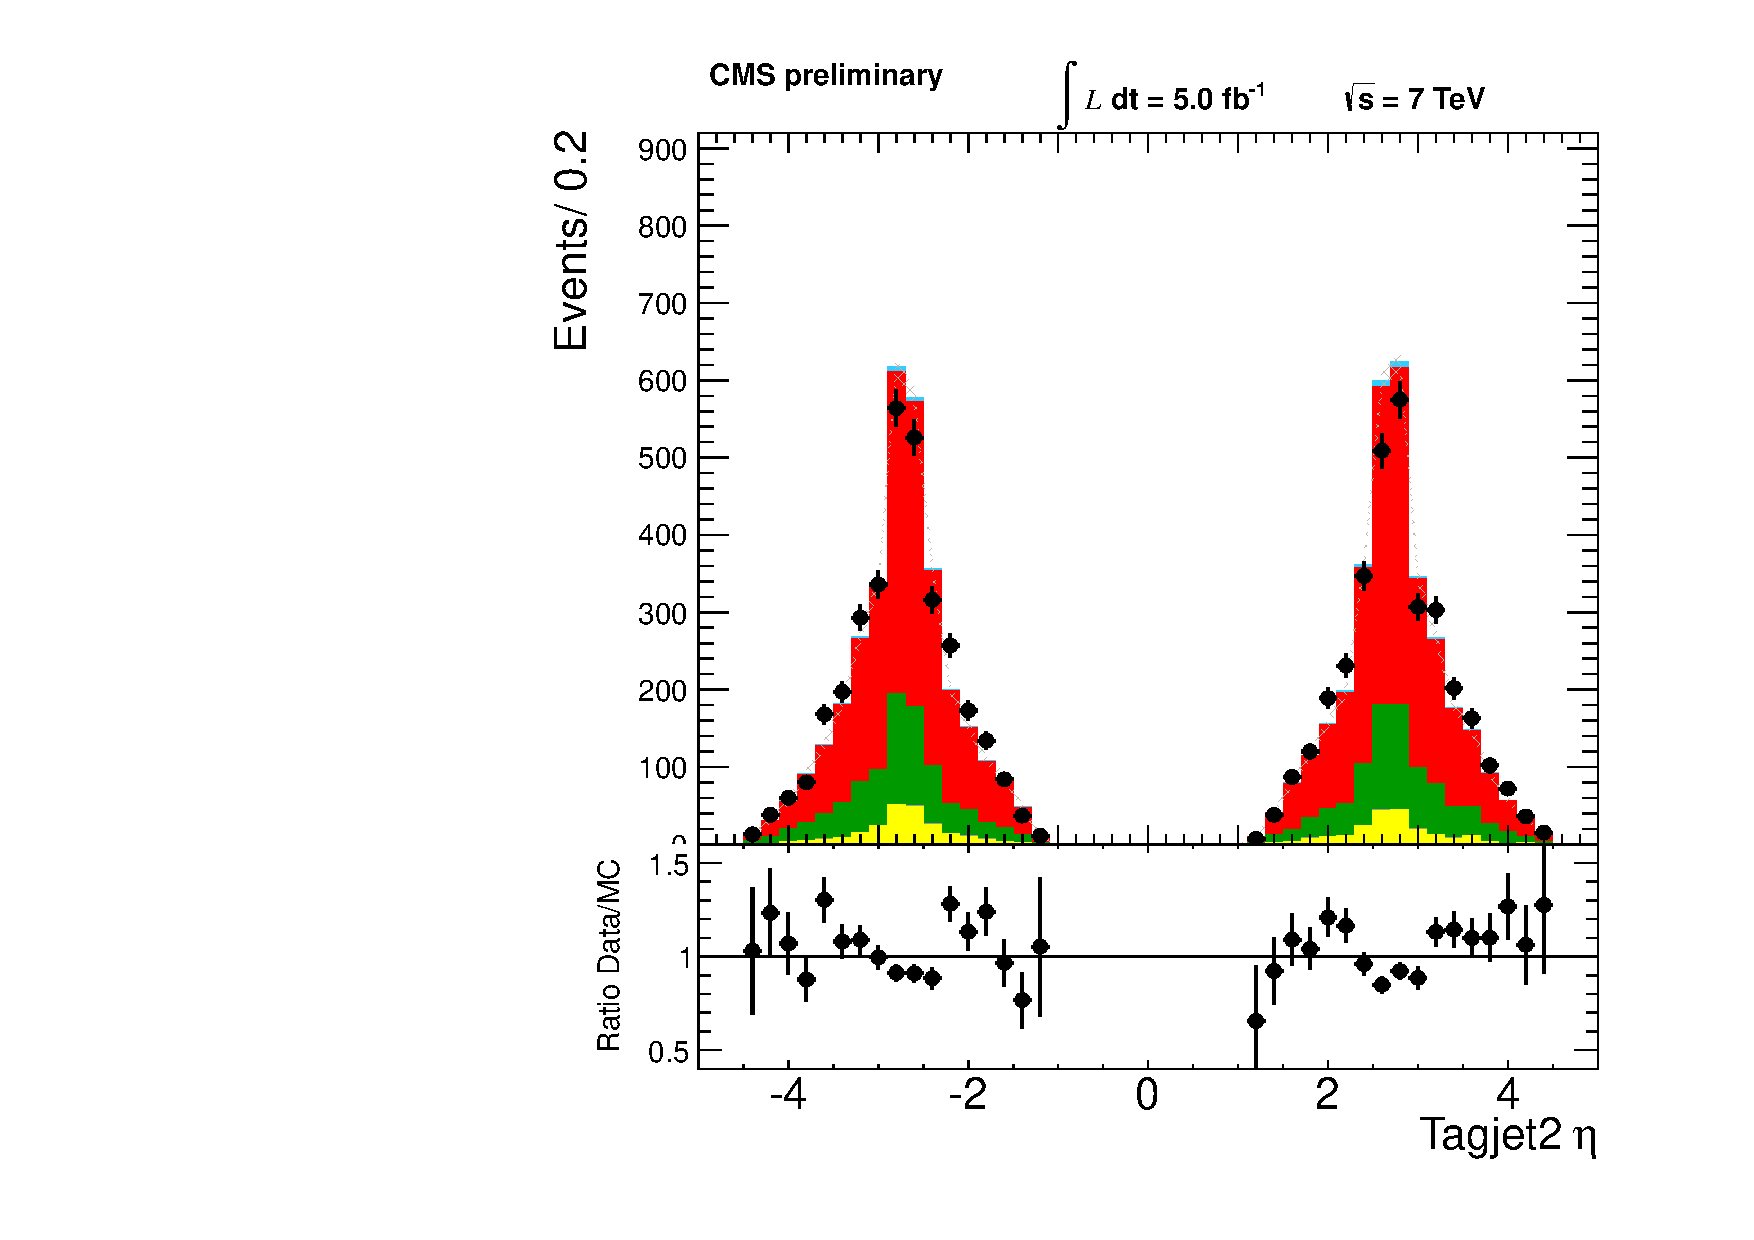
\includegraphics[width=0.49\textwidth]{figs/n-1_plots_mu/mu_vbftagjetb_eta.pdf}
    \caption{Comparison of the first (left) and second (right)
      VBF-tagged jet $\eta $ distributions from data and MC for the
    muon+jets selection.  }
\label{fig:mu_tagjet_eta}}
\end{figure}


%%%%%%%%%%%%%%%%%%%%%%%%%%%%
\begin{figure}[h!t]
  {\centering
    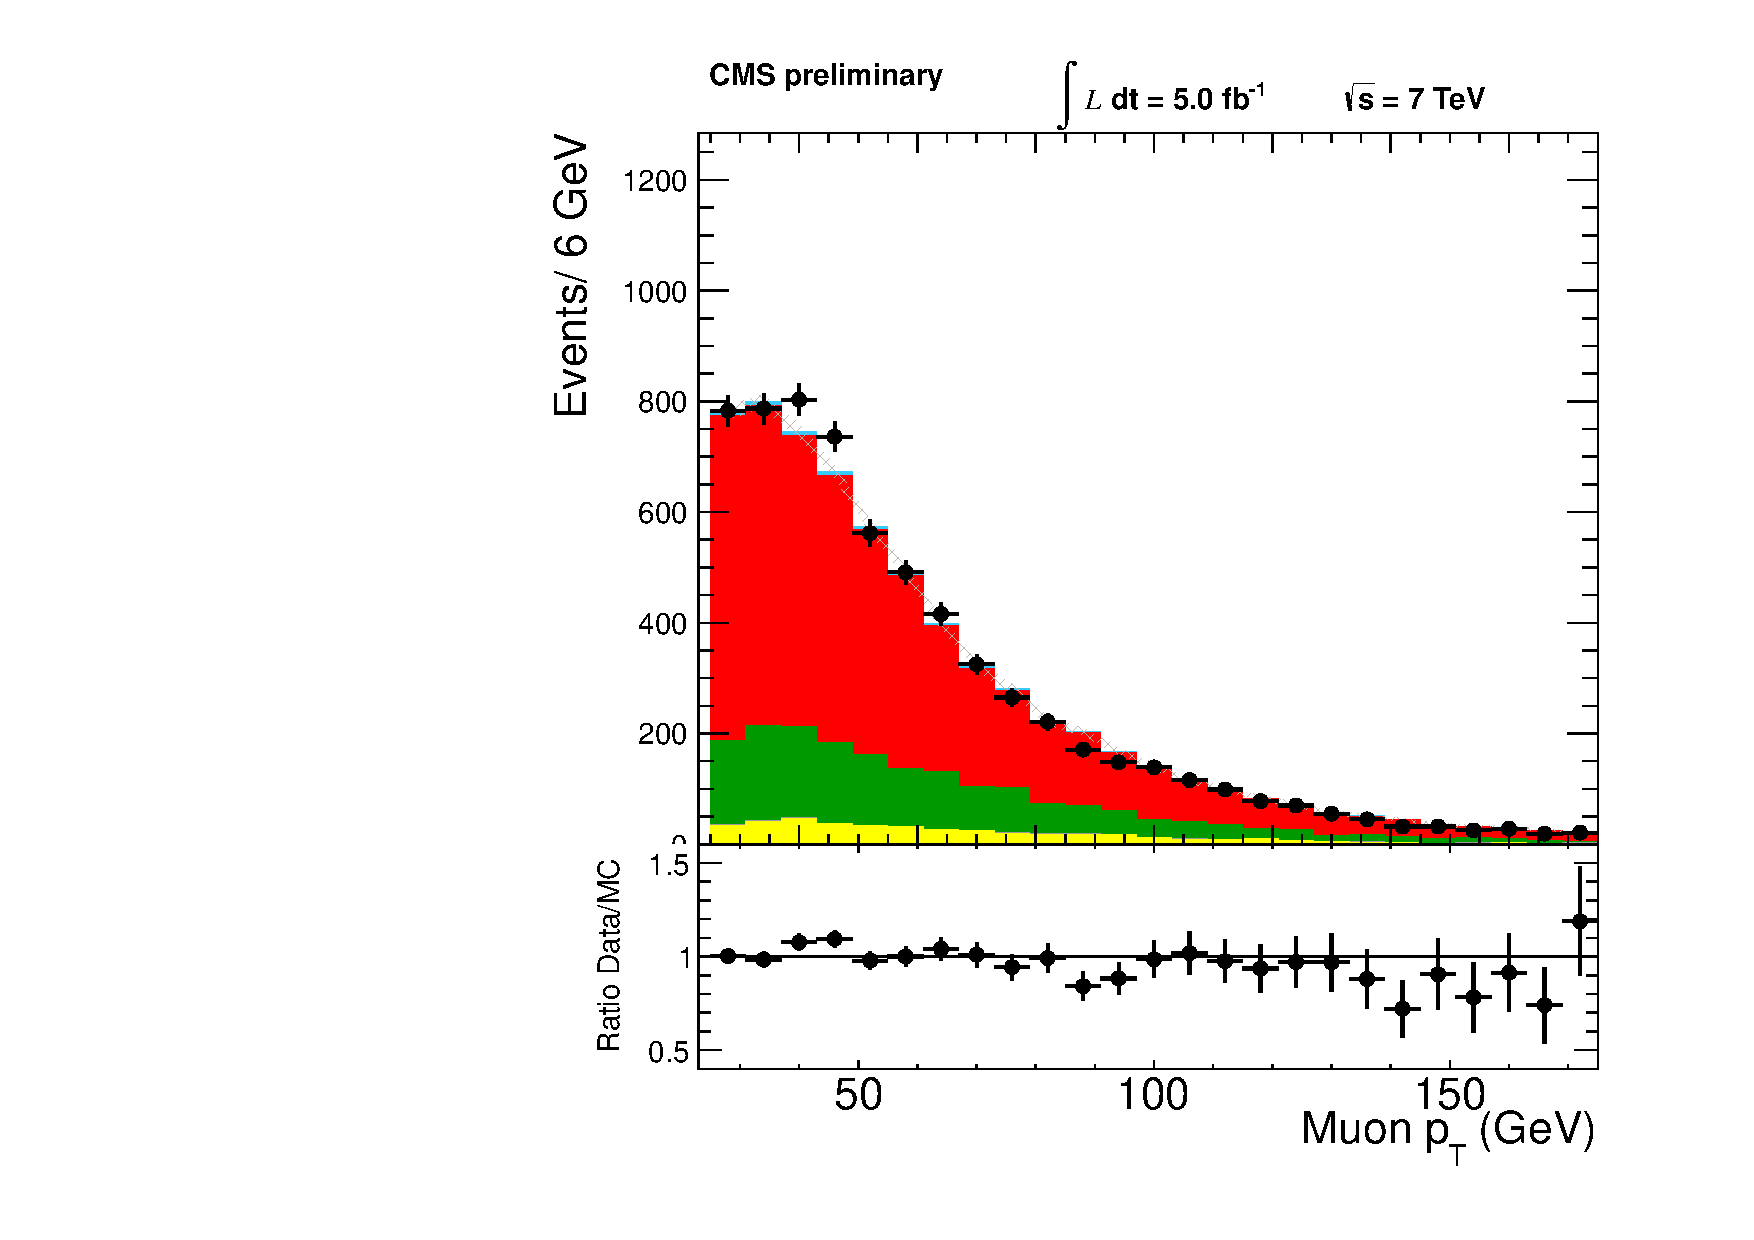
\includegraphics[width=0.49\textwidth]{figs/n-1_plots_mu/mu_W_muon_pt.pdf}
    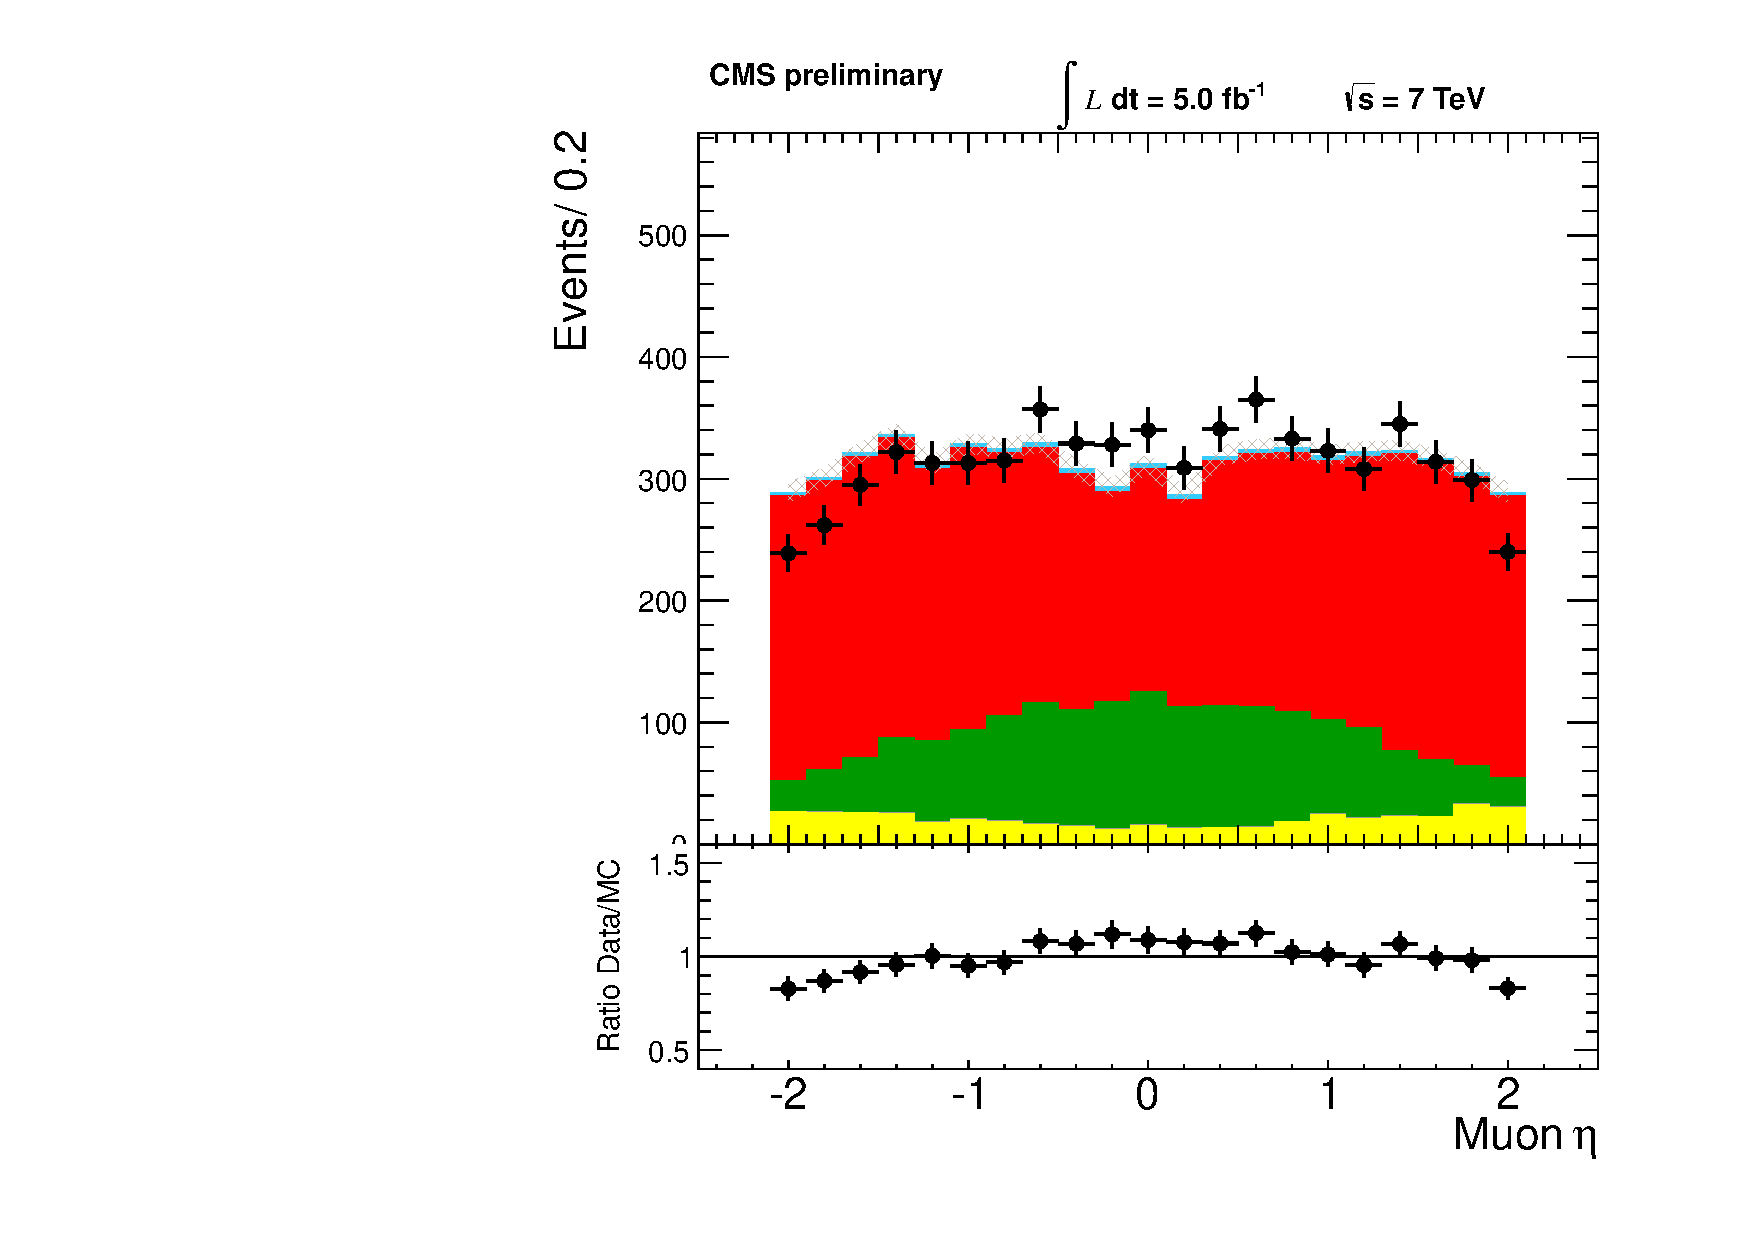
\includegraphics[width=0.49\textwidth]{figs/n-1_plots_mu/mu_W_muon_eta.pdf}
    \caption{Comparison of the muon $p_{T} $ (left) and the
    muon $\eta $ (right) distributions from data and MC for the
    muon+jets selection. 
    }
   \label{fig:mu_muon}}
\end{figure}

%%%%%%%%%%%%%%%%%%%%%%%%%%%%
\begin{figure}[h!t]
  {\centering
    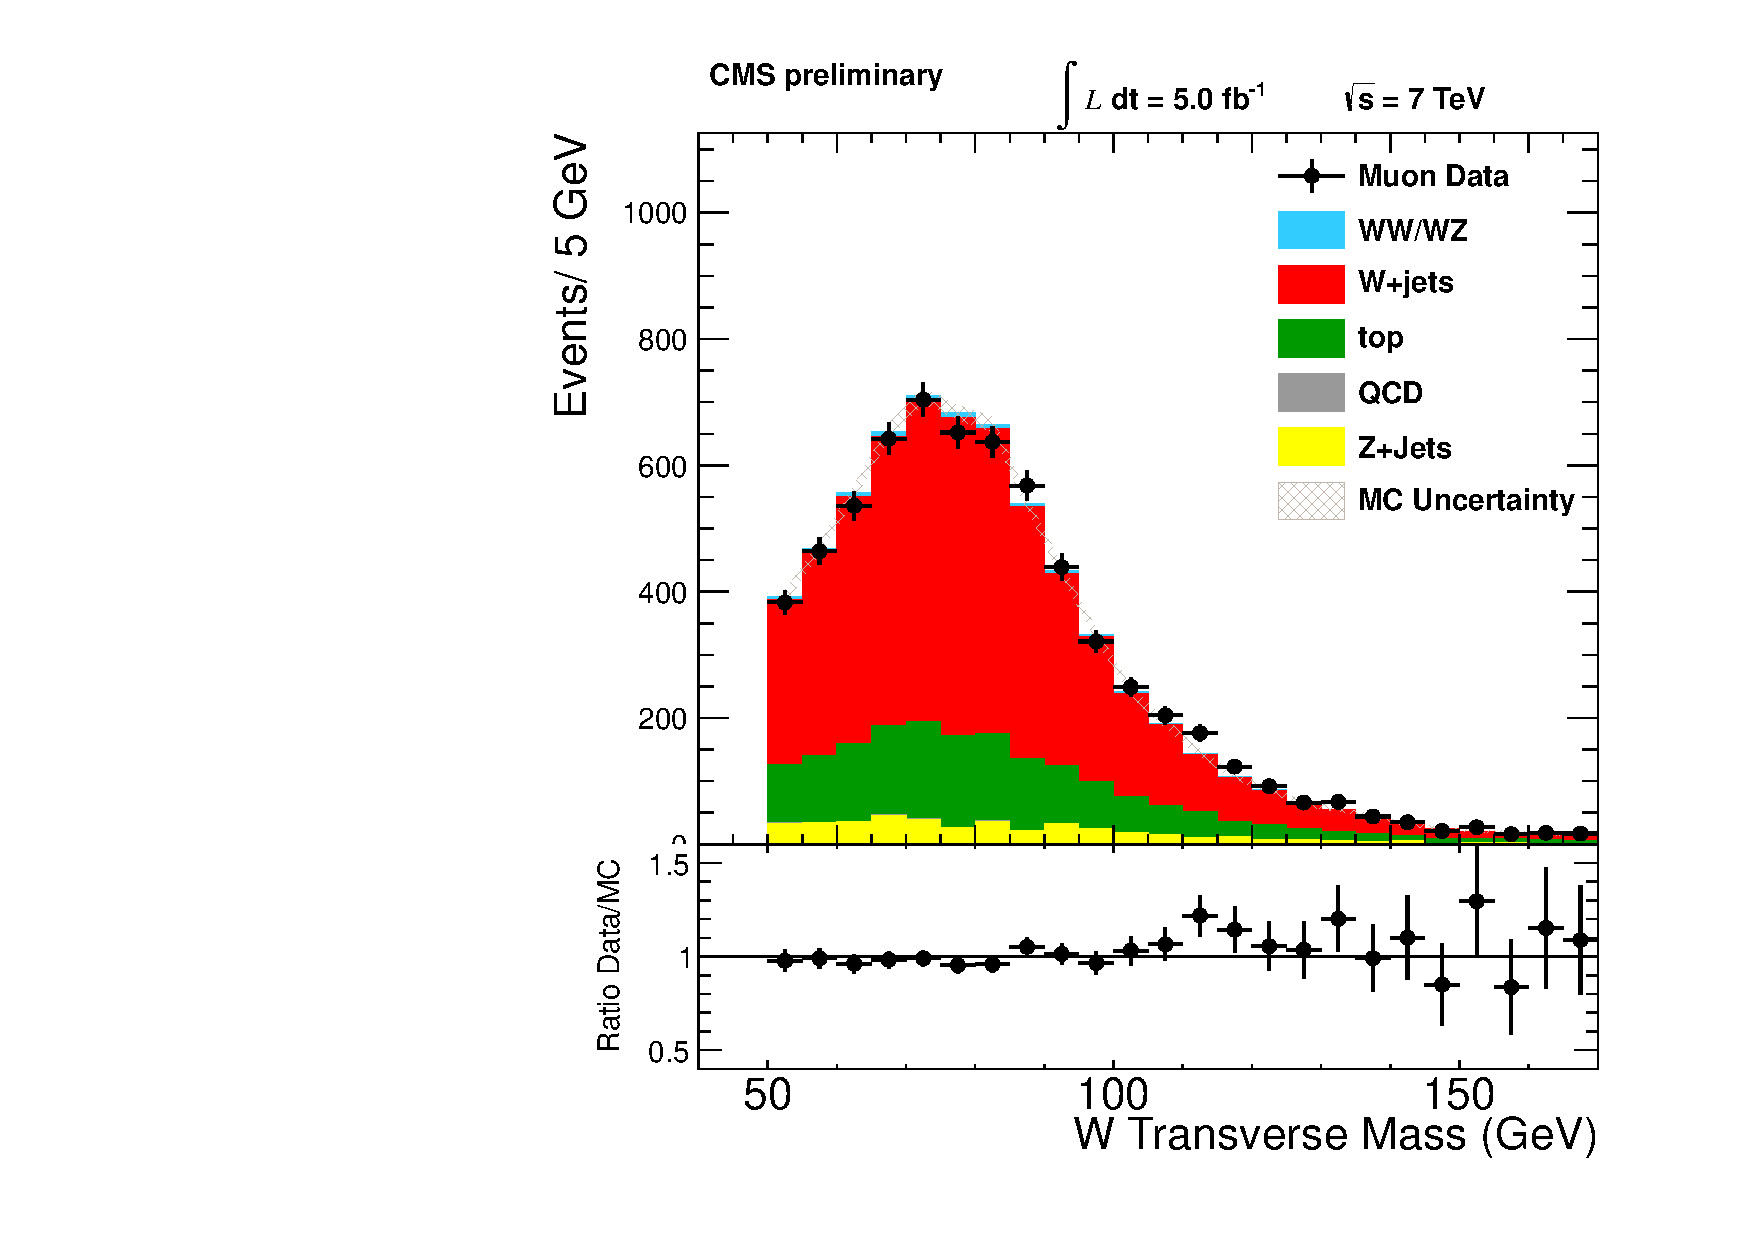
\includegraphics[width=0.49\textwidth]{figs/n-1_plots_mu/mu_vbf_W_mt.pdf}
    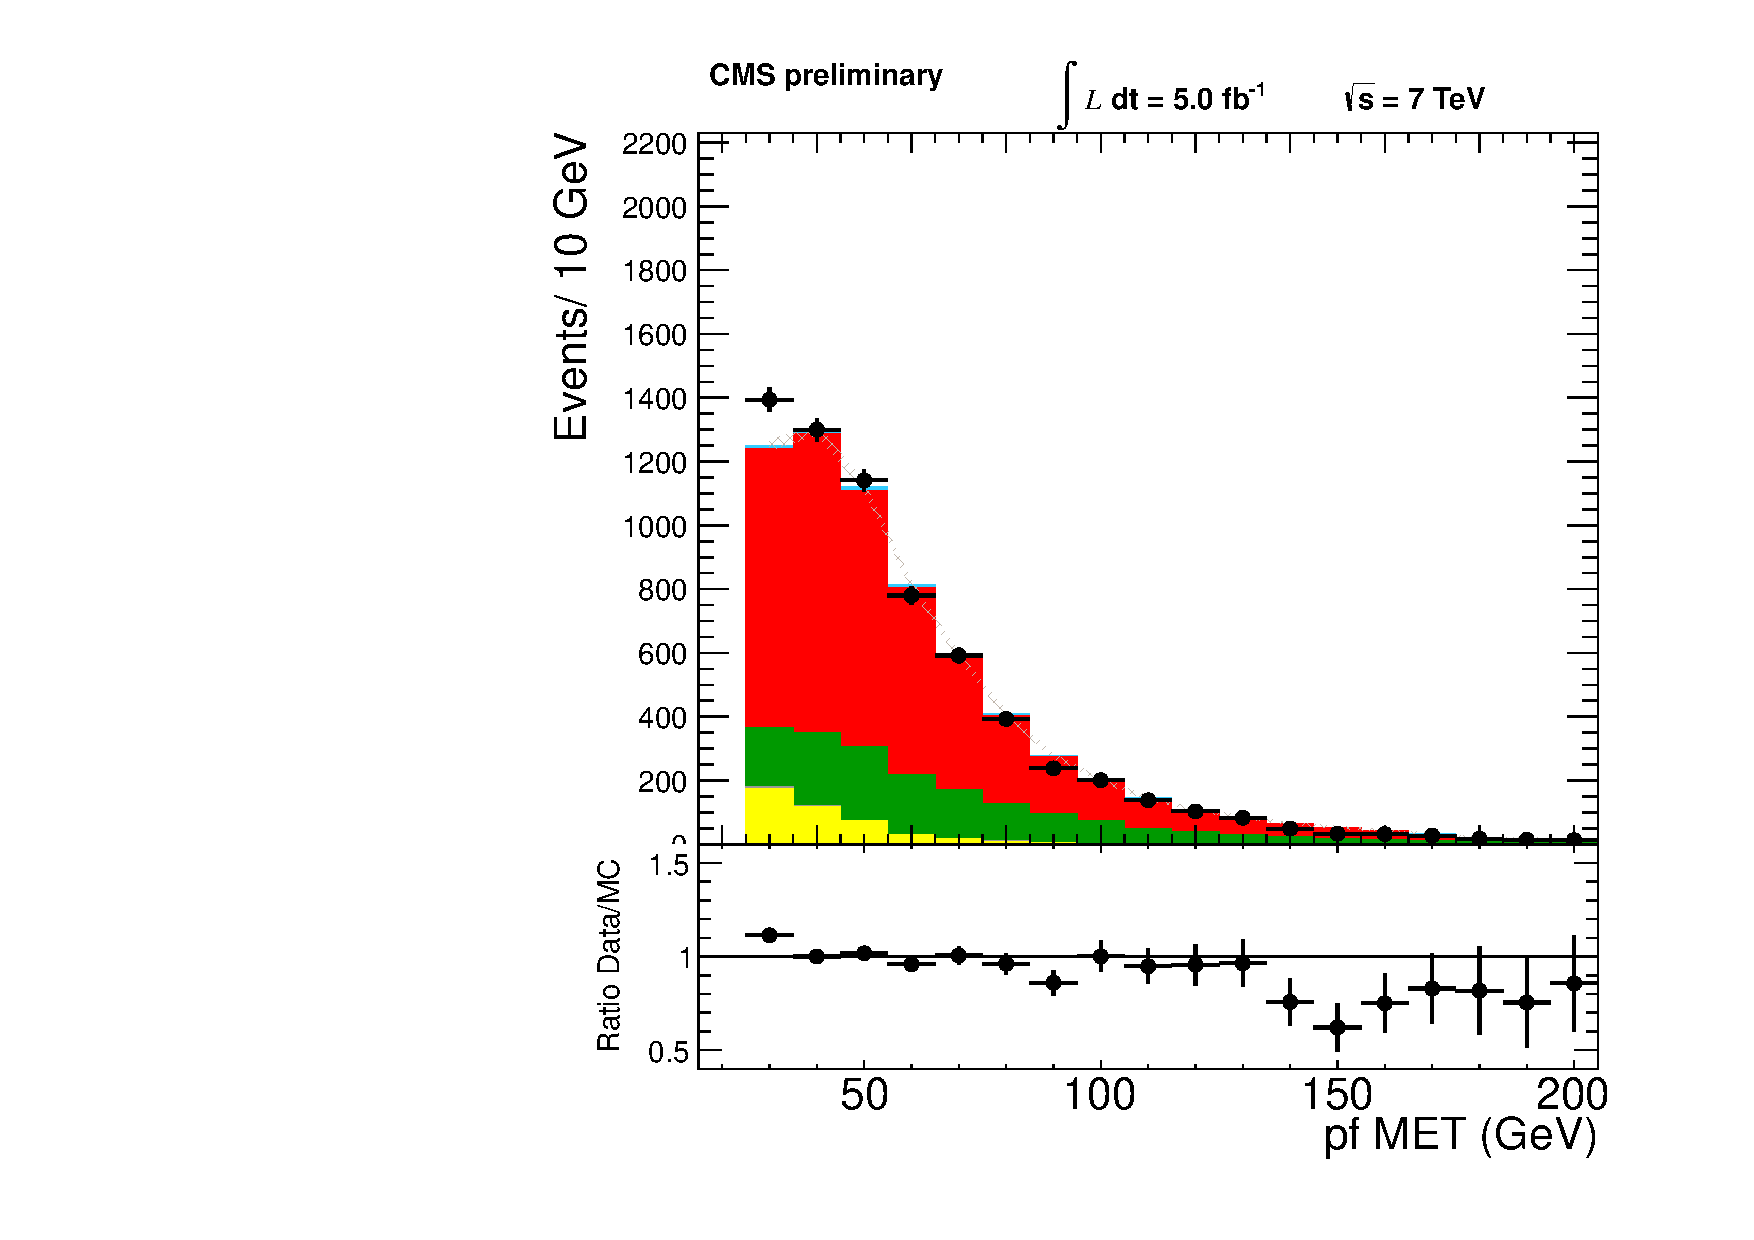
\includegraphics[width=0.49\textwidth]{figs/n-1_plots_mu/mu_event_met_pfmet.pdf}
    \caption{Comparison of the distributions from data and MC of the
     transverse mass of the muon / MET system (left) and the MET (right)
    for the muon+jets selection.
    }
    \label{fig:mu_W_Mt}}
\end{figure}
%%%%%%%%%%%%%%%%%%%%%%%%%%%%
\begin{figure}[h!t]
  {\centering
    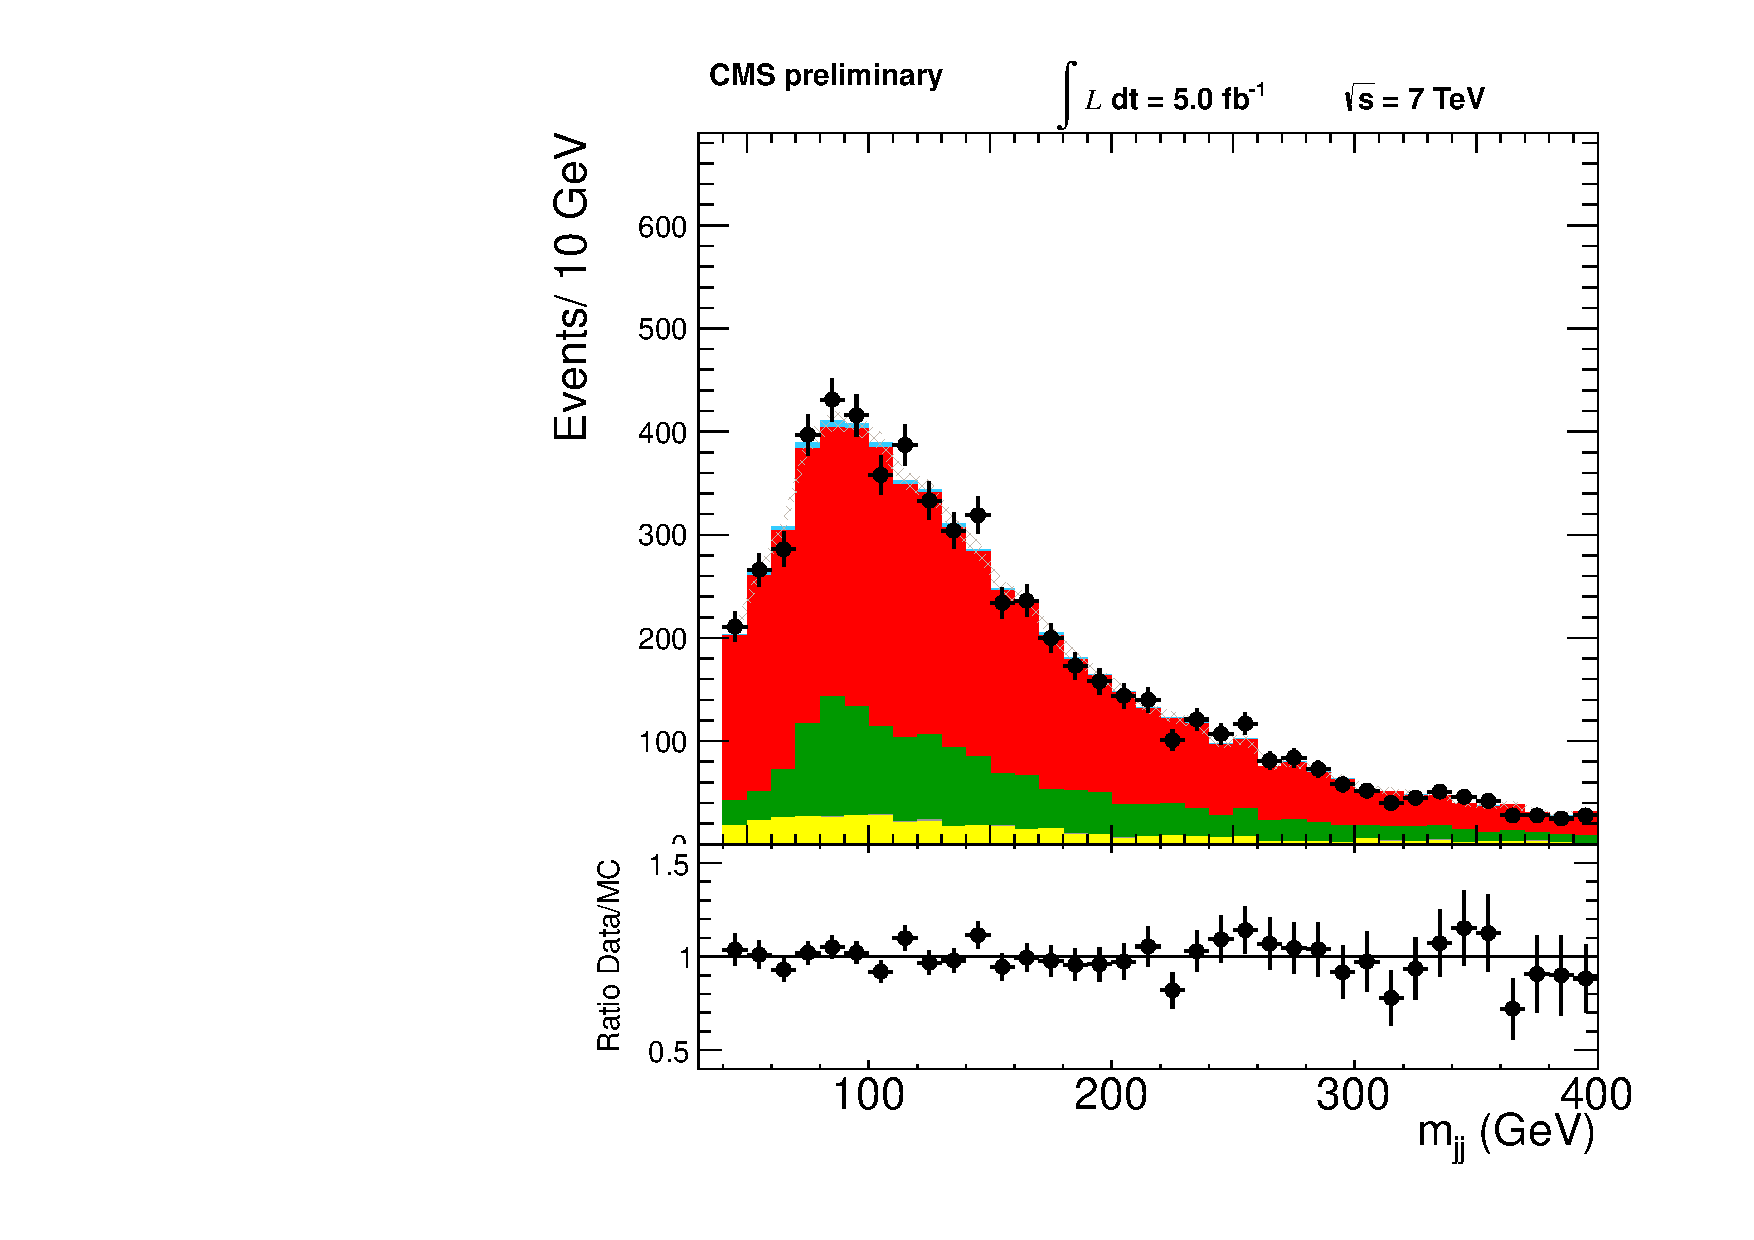
\includegraphics[width=0.49\textwidth]{figs/n-1_plots_mu/mu_vbfwjjmass.pdf}
    \caption{Comparison of the hadronic W dijet mass ($m_{JJ}$)
      distributions from data and MC for the muon+jets selection. }
    \label{fig:mu_mjj}}
\end{figure}

%%%%%%%%%%%%%%%%%%%%%%%%%%%%
%%%%%%%%%%%%%%%%%%%%%%%%%%%%
\begin{figure}[h!t]
  {\centering
    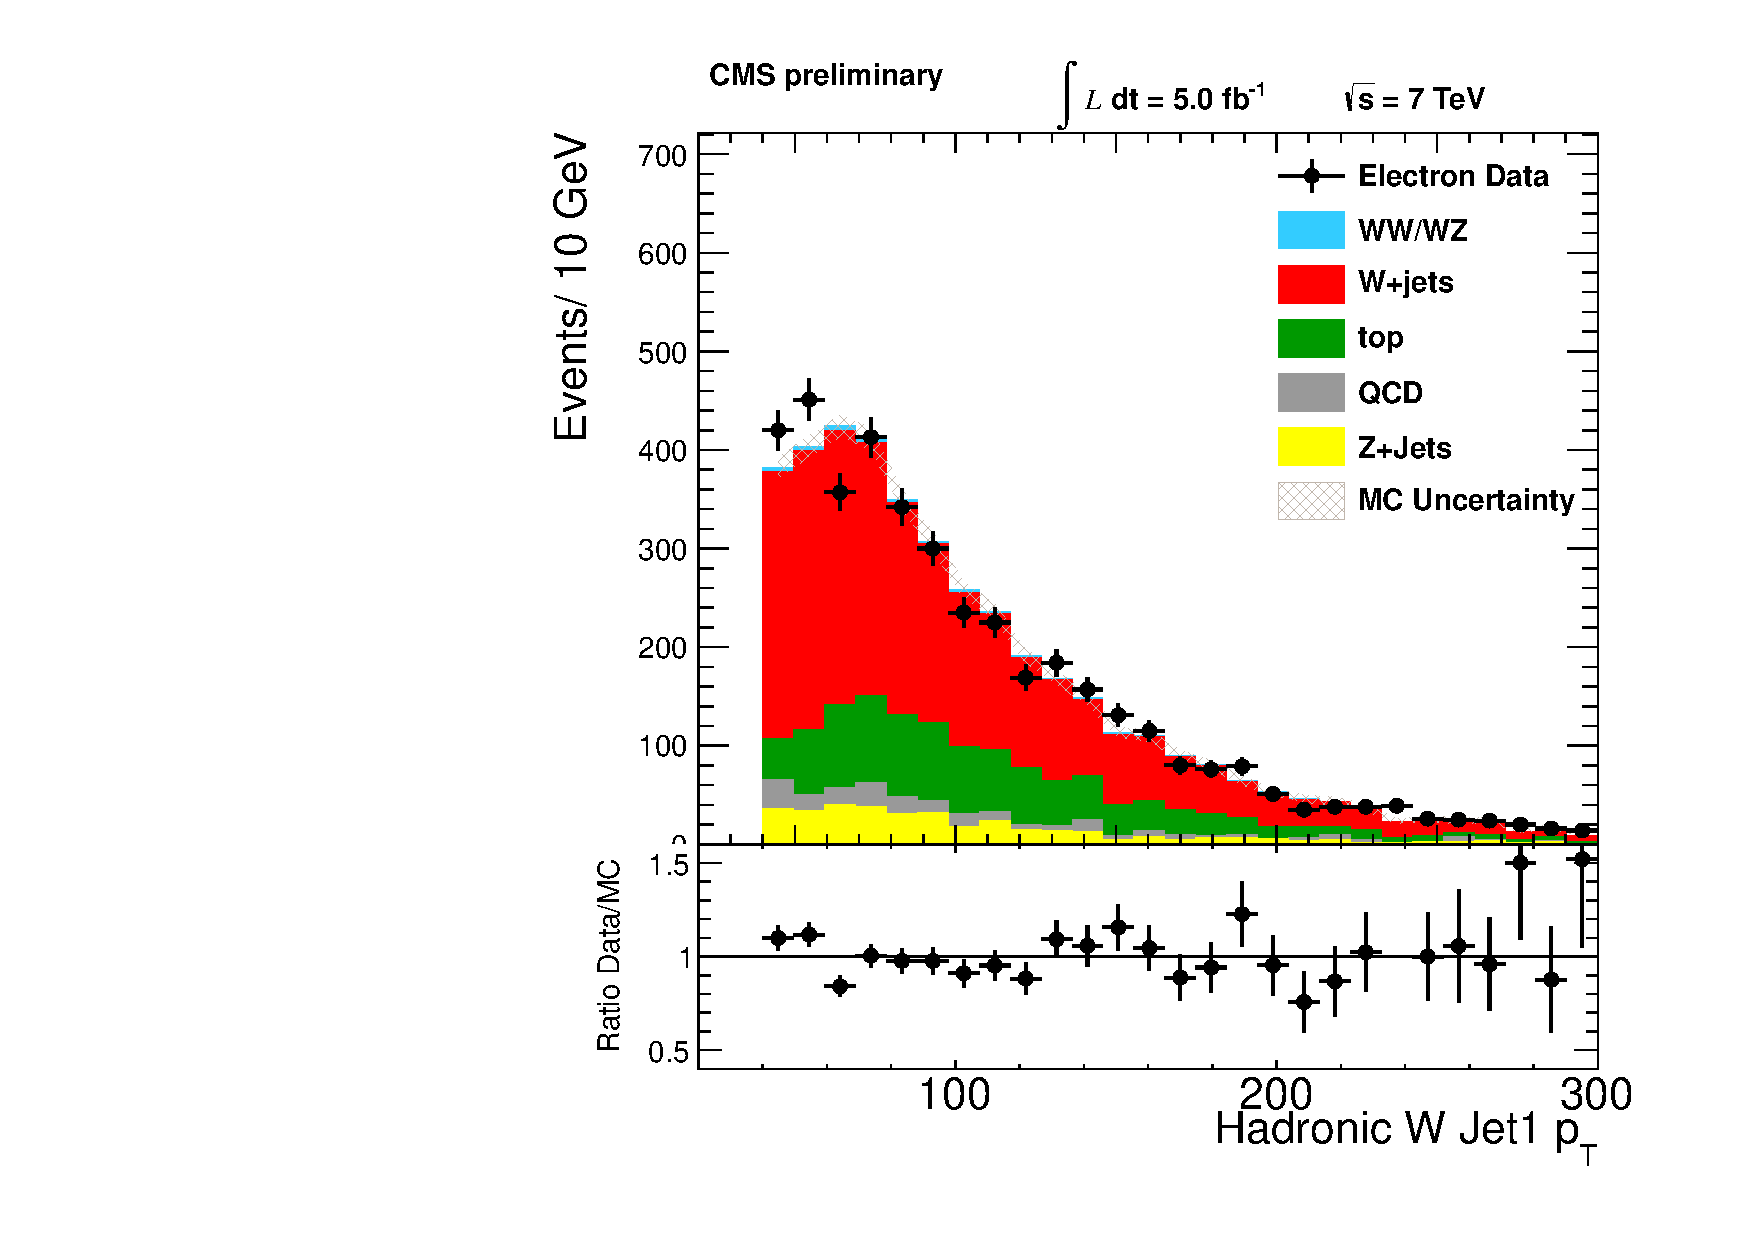
\includegraphics[width=0.49\textwidth]{figs/n-1_plots_el/el_vbfwjeta_pt.pdf}
    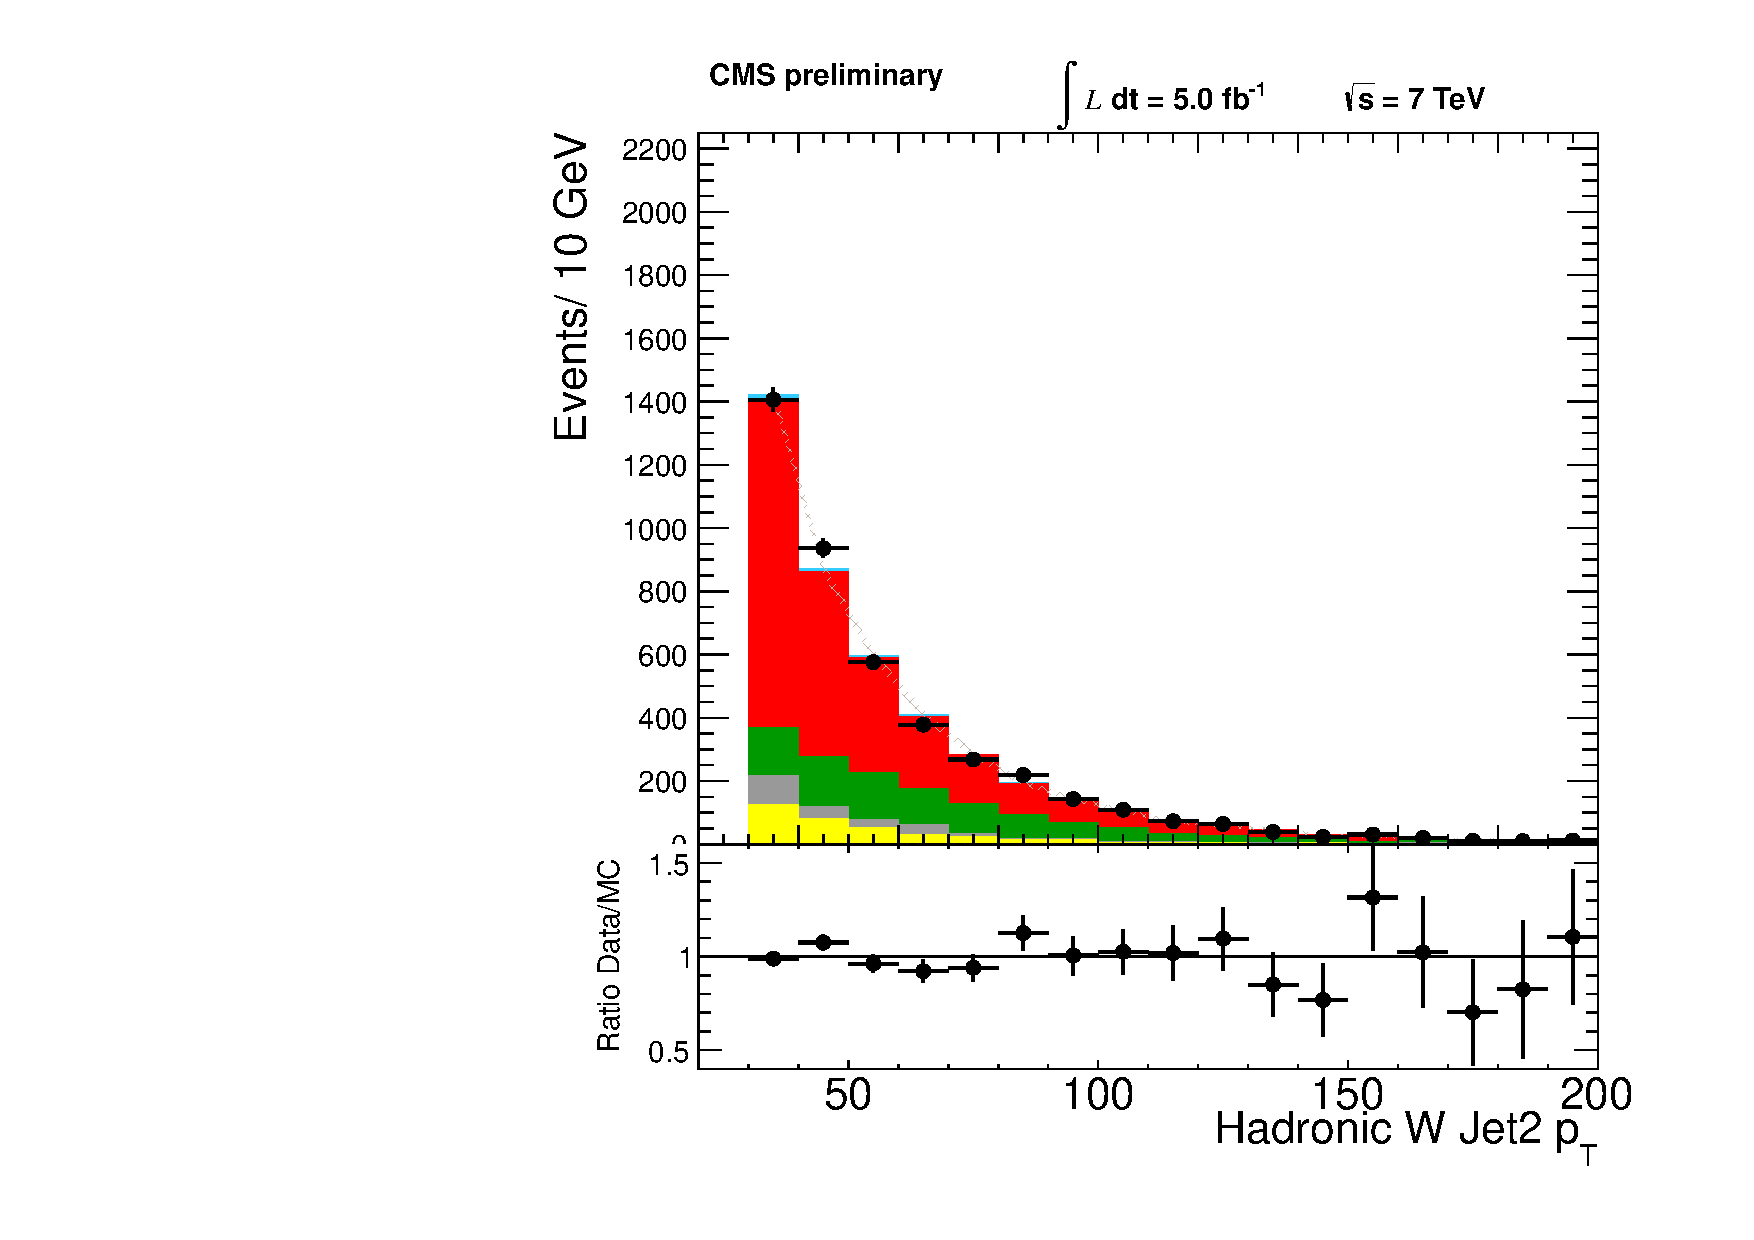
\includegraphics[width=0.49\textwidth]{figs/n-1_plots_el/el_vbfwjetb_pt.pdf}
    \caption{Comparison of the first (left) and second (right)
    hadronic W jet $\eta $ distributions from data and MC for the
    electron+jets selection.}
    \label{fig:el_jet_pt}}
\end{figure}
%%%%%%%%%%%%%%%%%%%%%%%%%%%%
\begin{figure}[h!t]
  {\centering
    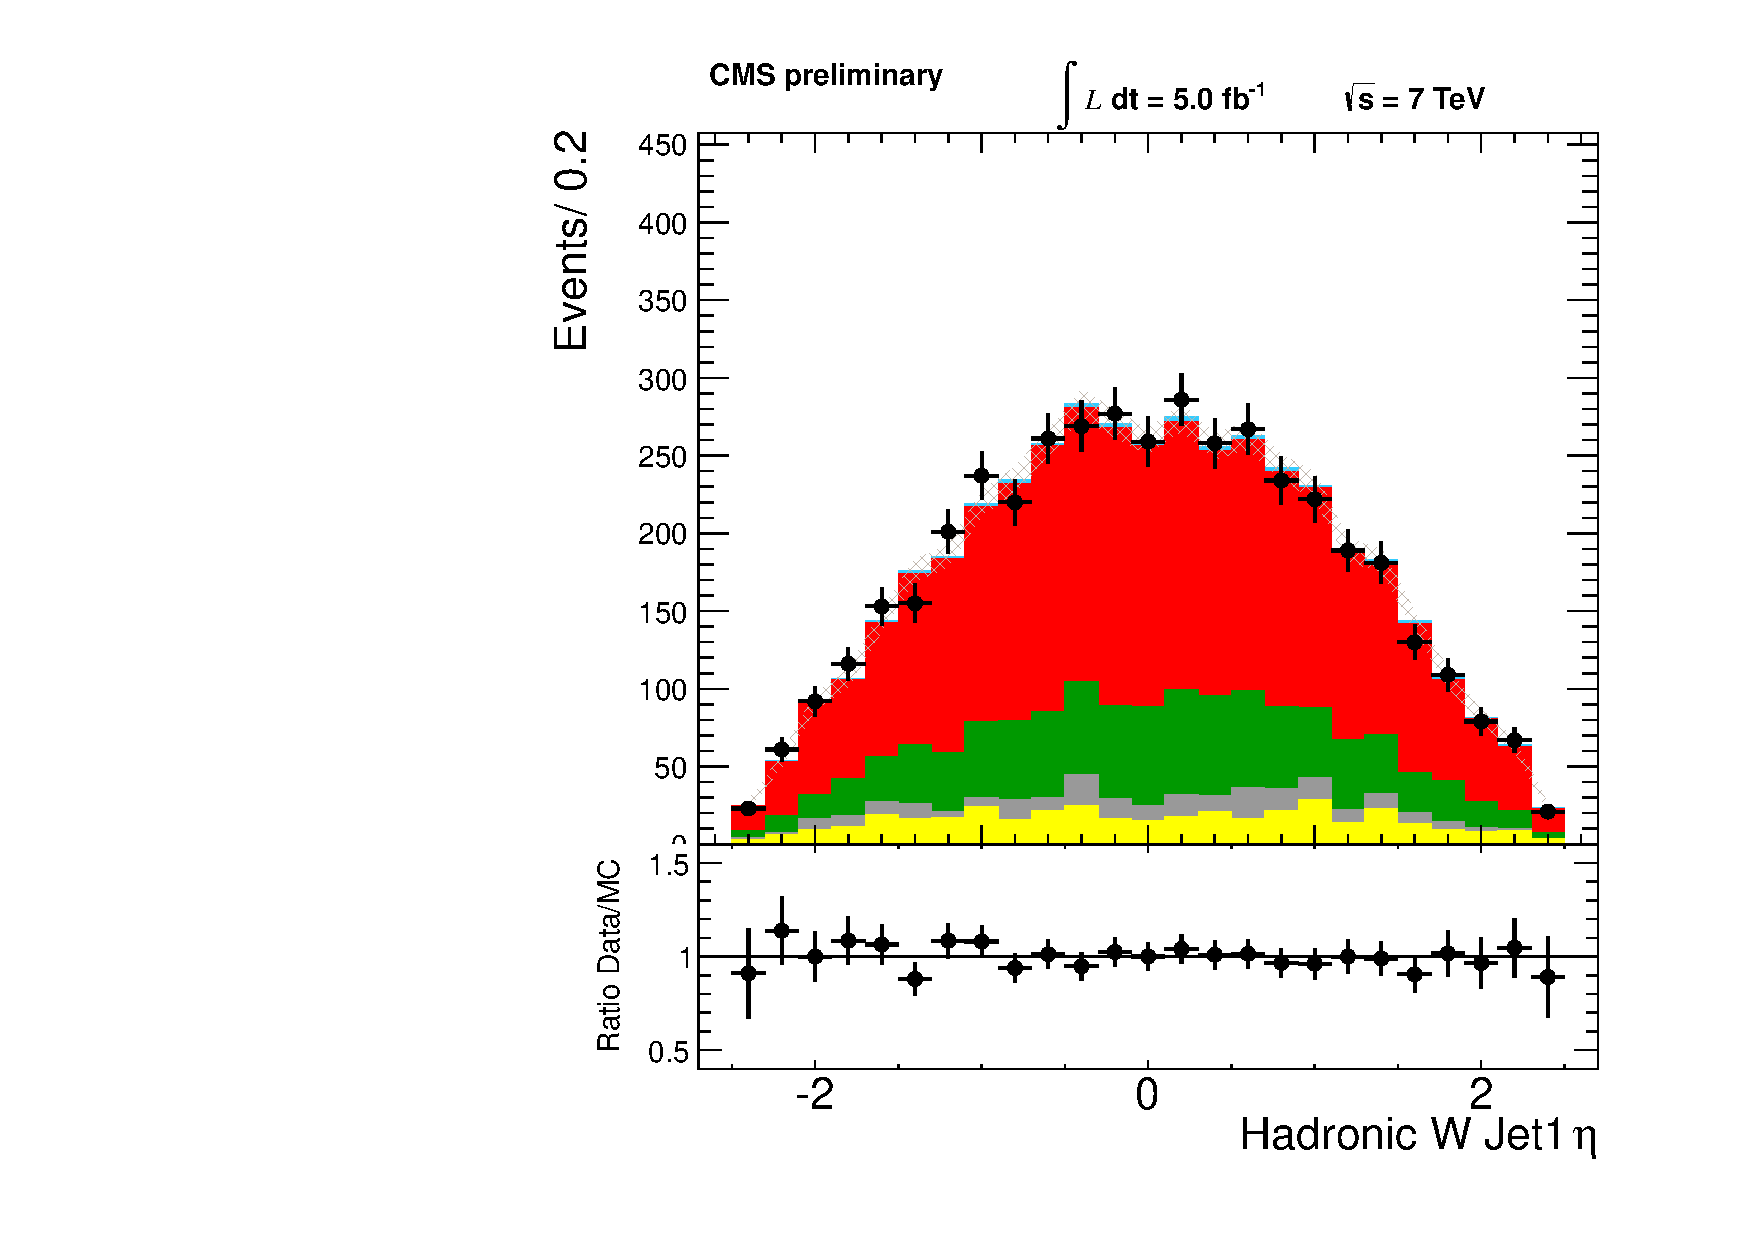
\includegraphics[width=0.49\textwidth]{figs/n-1_plots_el/el_vbfwjeta_eta.pdf}
    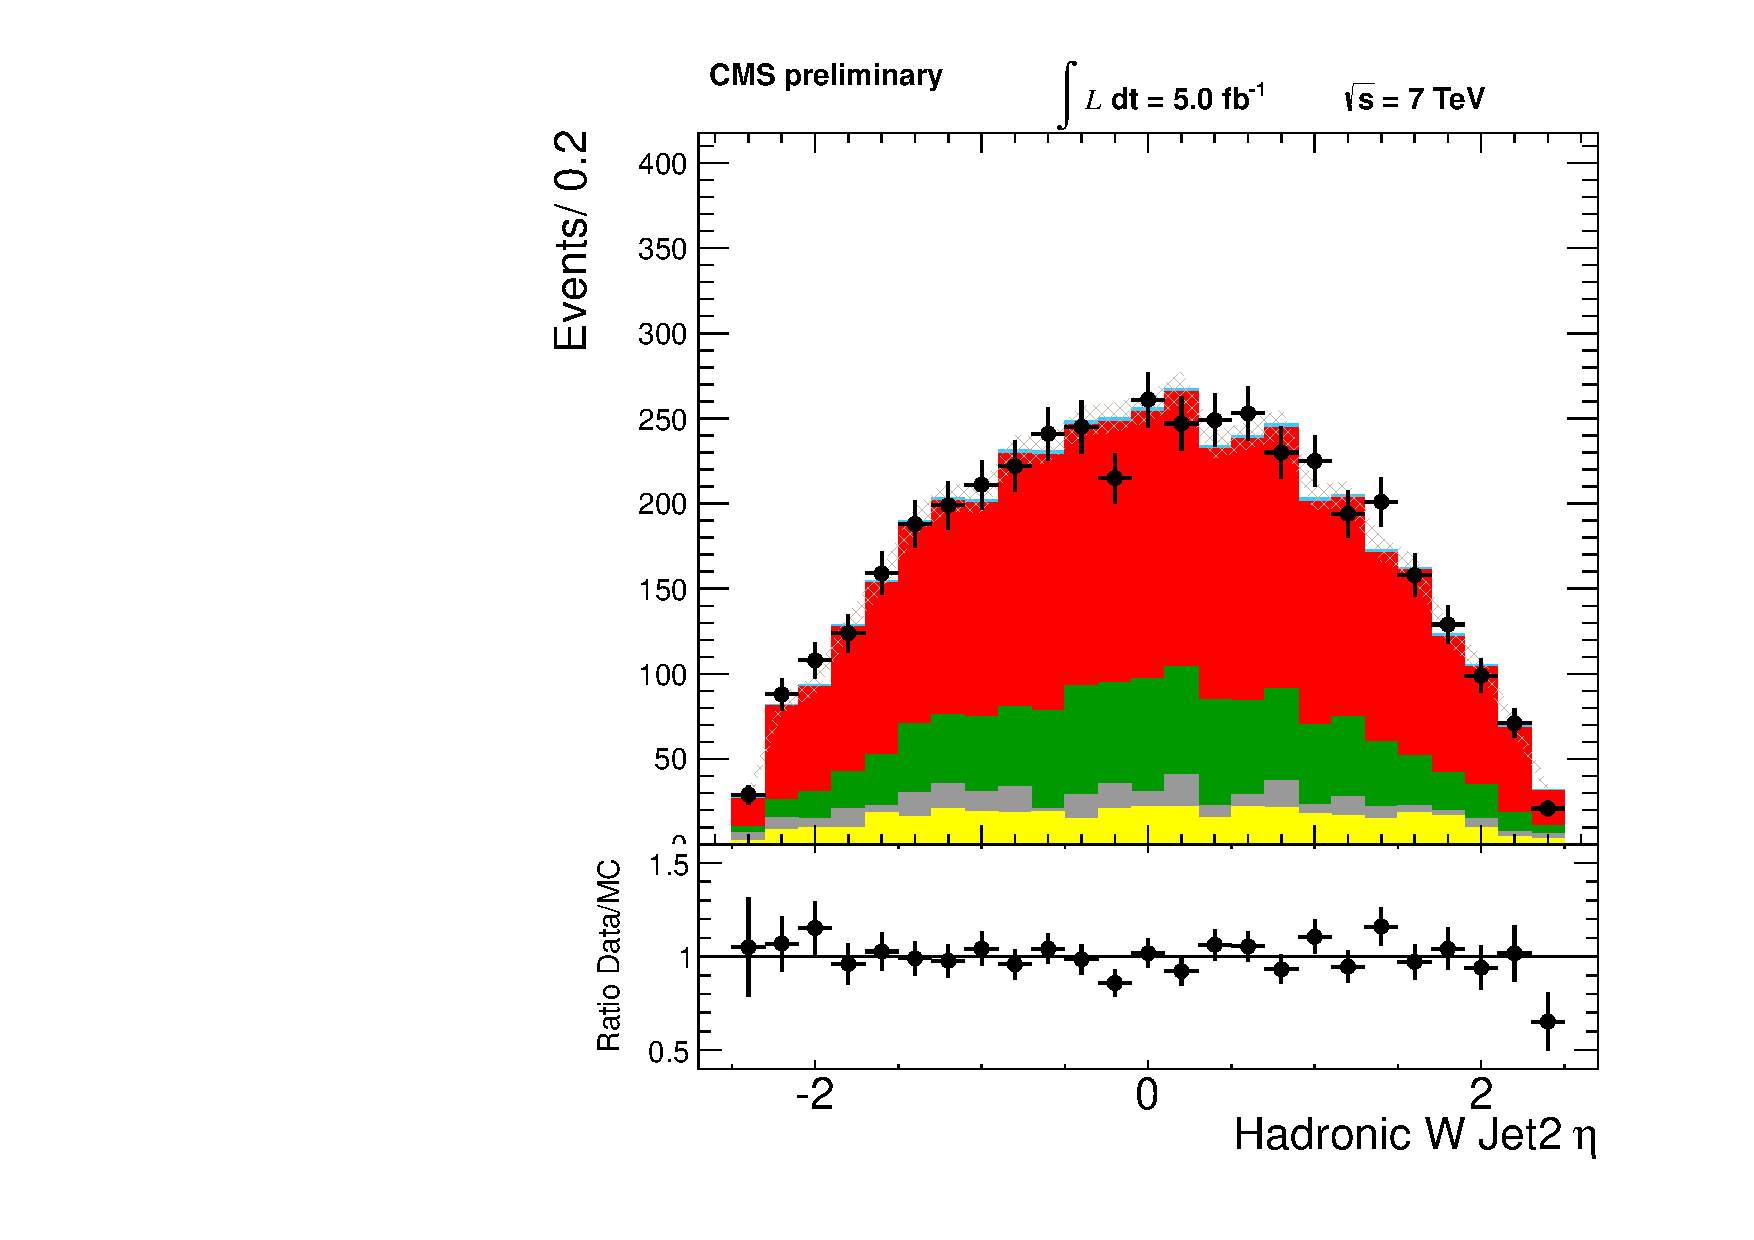
\includegraphics[width=0.49\textwidth]{figs/n-1_plots_el/el_vbfwjetb_eta.pdf}
    \caption{Comparison of the first (left) and second (right)
    hadronic W jet $\eta $ distributions from data and MC for the
    electron+jets selection.}
    \label{fig:el_jet_eta}}
\end{figure}

%%%%%%%%%%%%%%%%%%%%%%%%%%%%
\begin{figure}[h!t]
  {\centering
    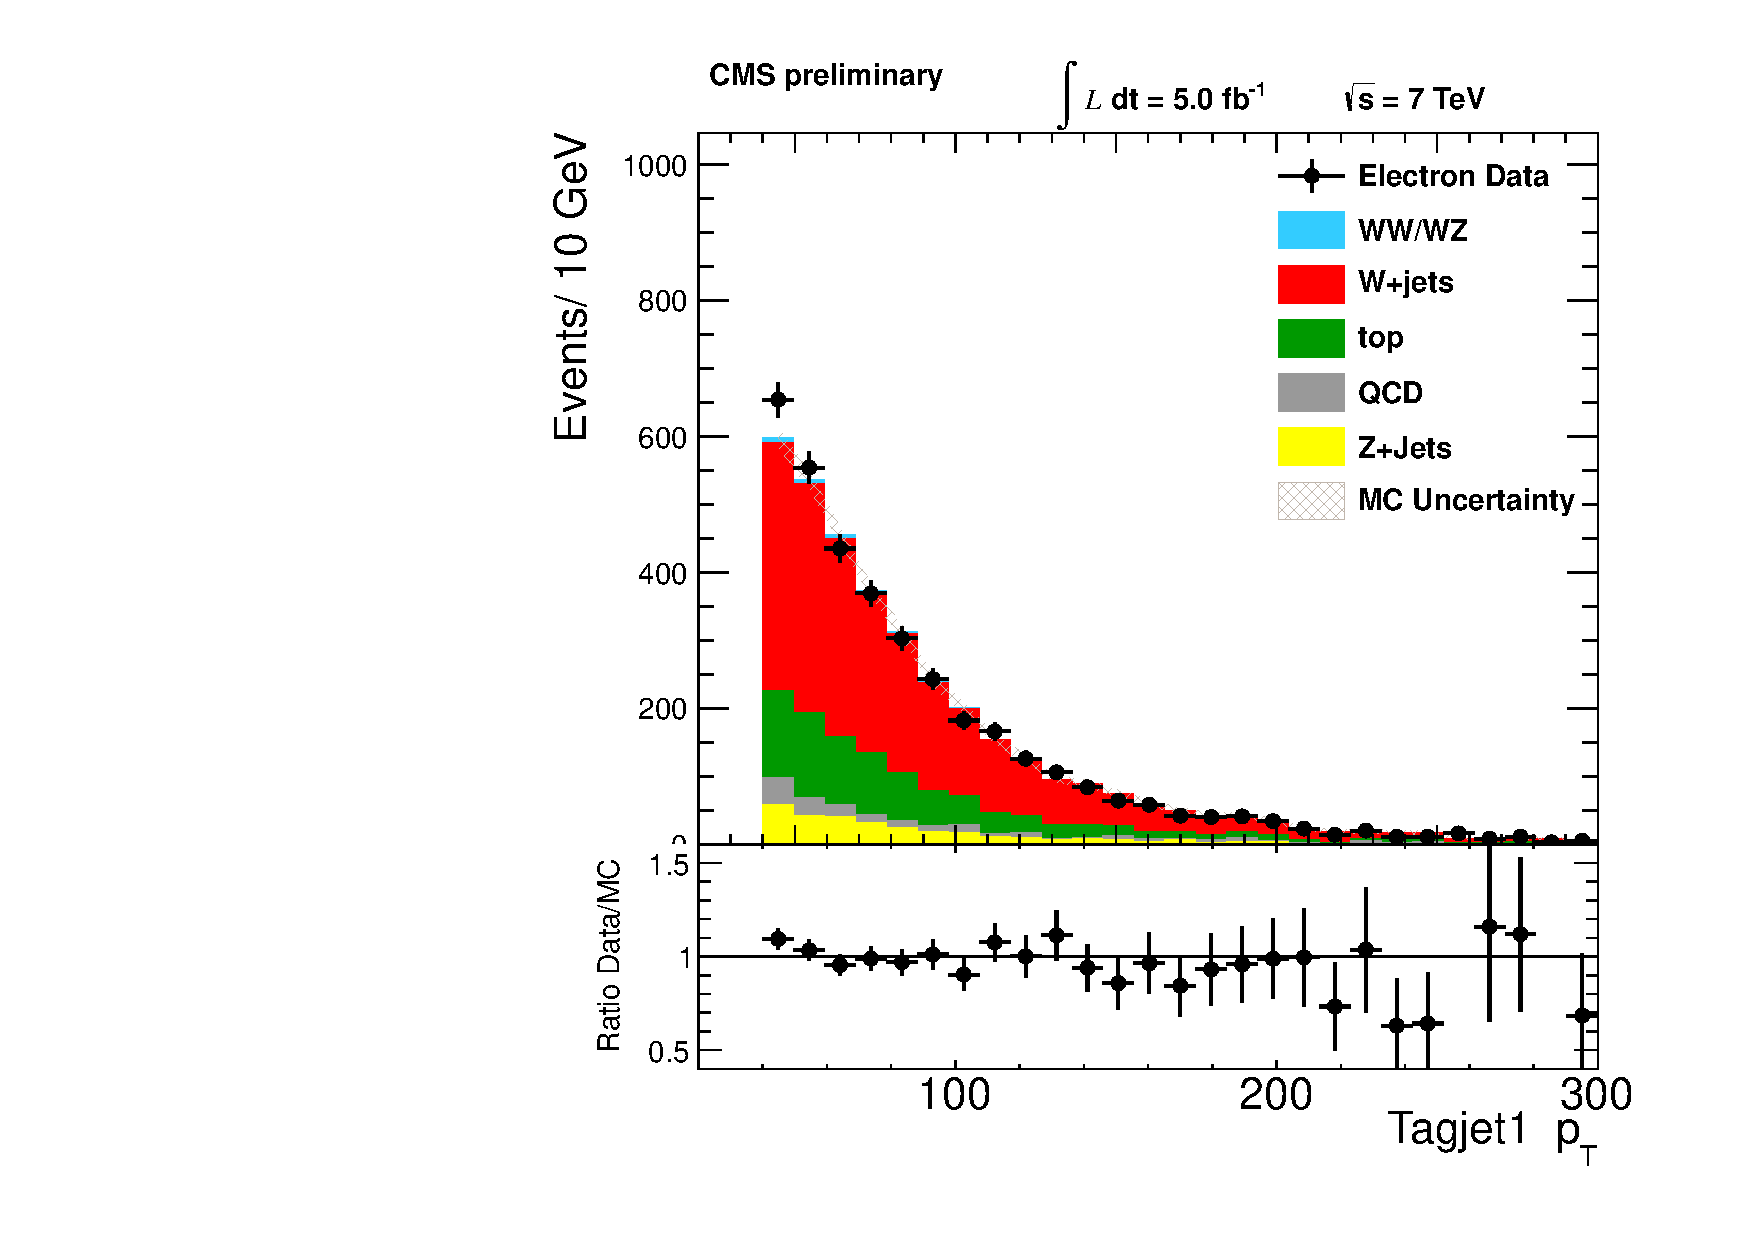
\includegraphics[width=0.49\textwidth]{figs/n-1_plots_el/el_vbftagjeta_pt.pdf}
    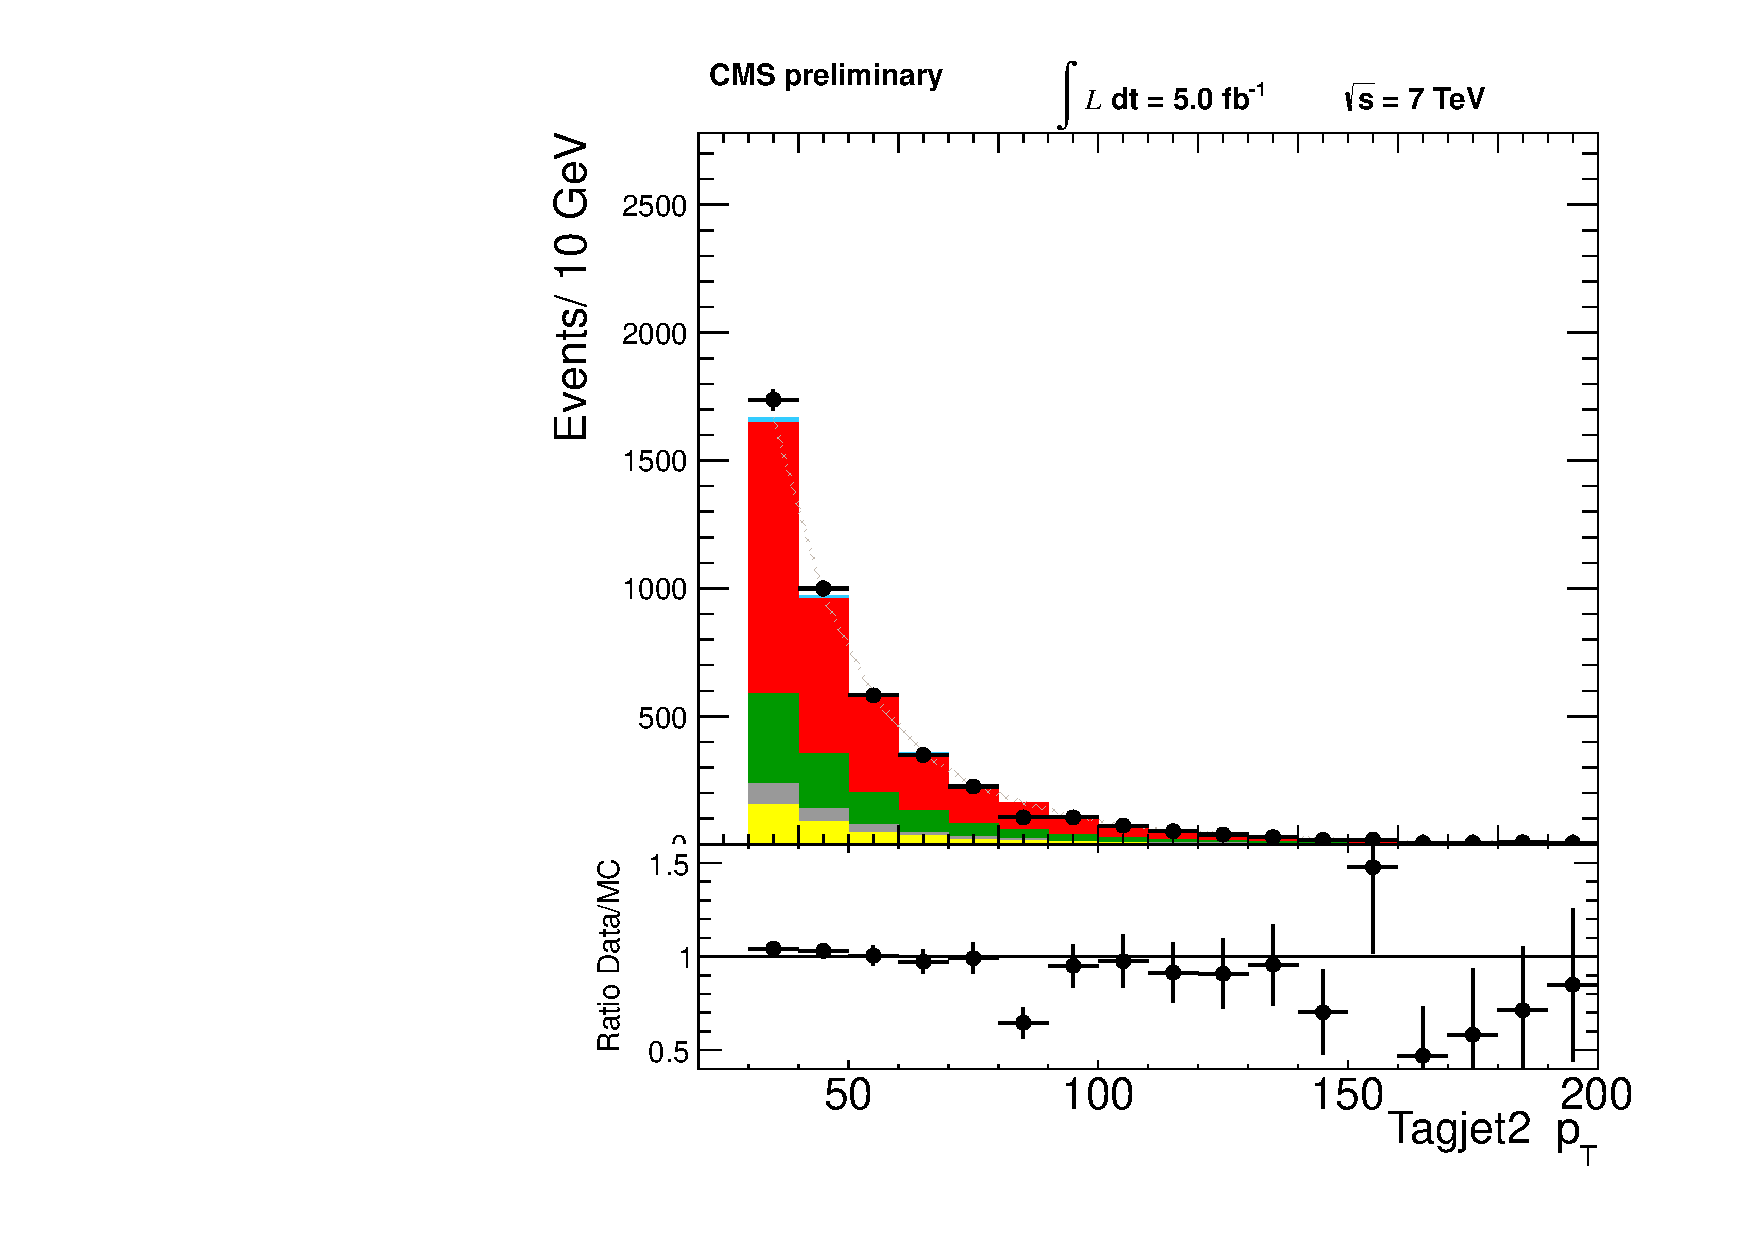
\includegraphics[width=0.49\textwidth]{figs/n-1_plots_el/el_vbftagjetb_pt.pdf}
    \caption{Comparison of the first (left) and second (right)
      VBF-tagged jet $p_{T}$ distributions from data and MC for the
      electron+jets selection.}
    \label{fig:el_tagjet_pt}}
\end{figure}

%%%%%%%%%%%%%%%%%%%%%%%%%%%%
\begin{figure}[h!t]
  {\centering
    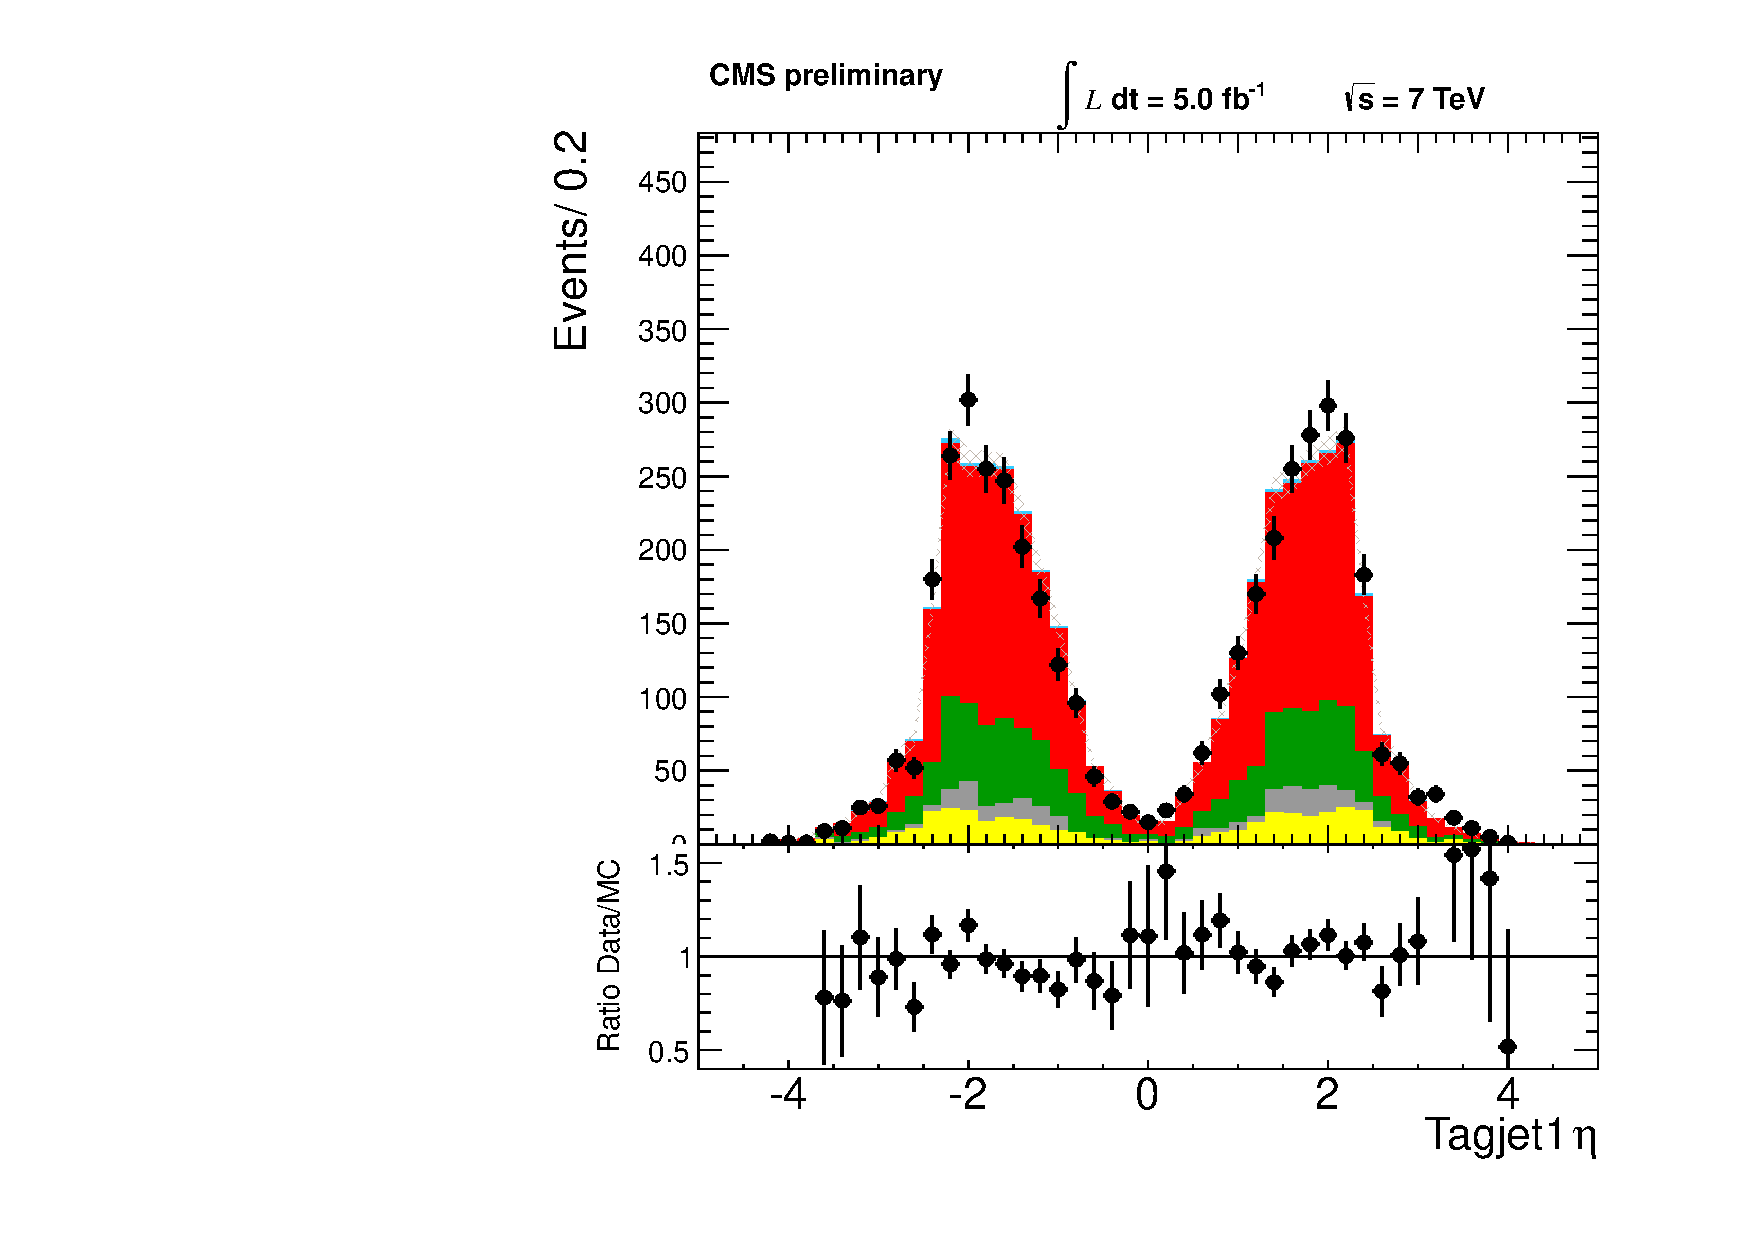
\includegraphics[width=0.49\textwidth]{figs/n-1_plots_el/el_vbftagjeta_eta.pdf}
    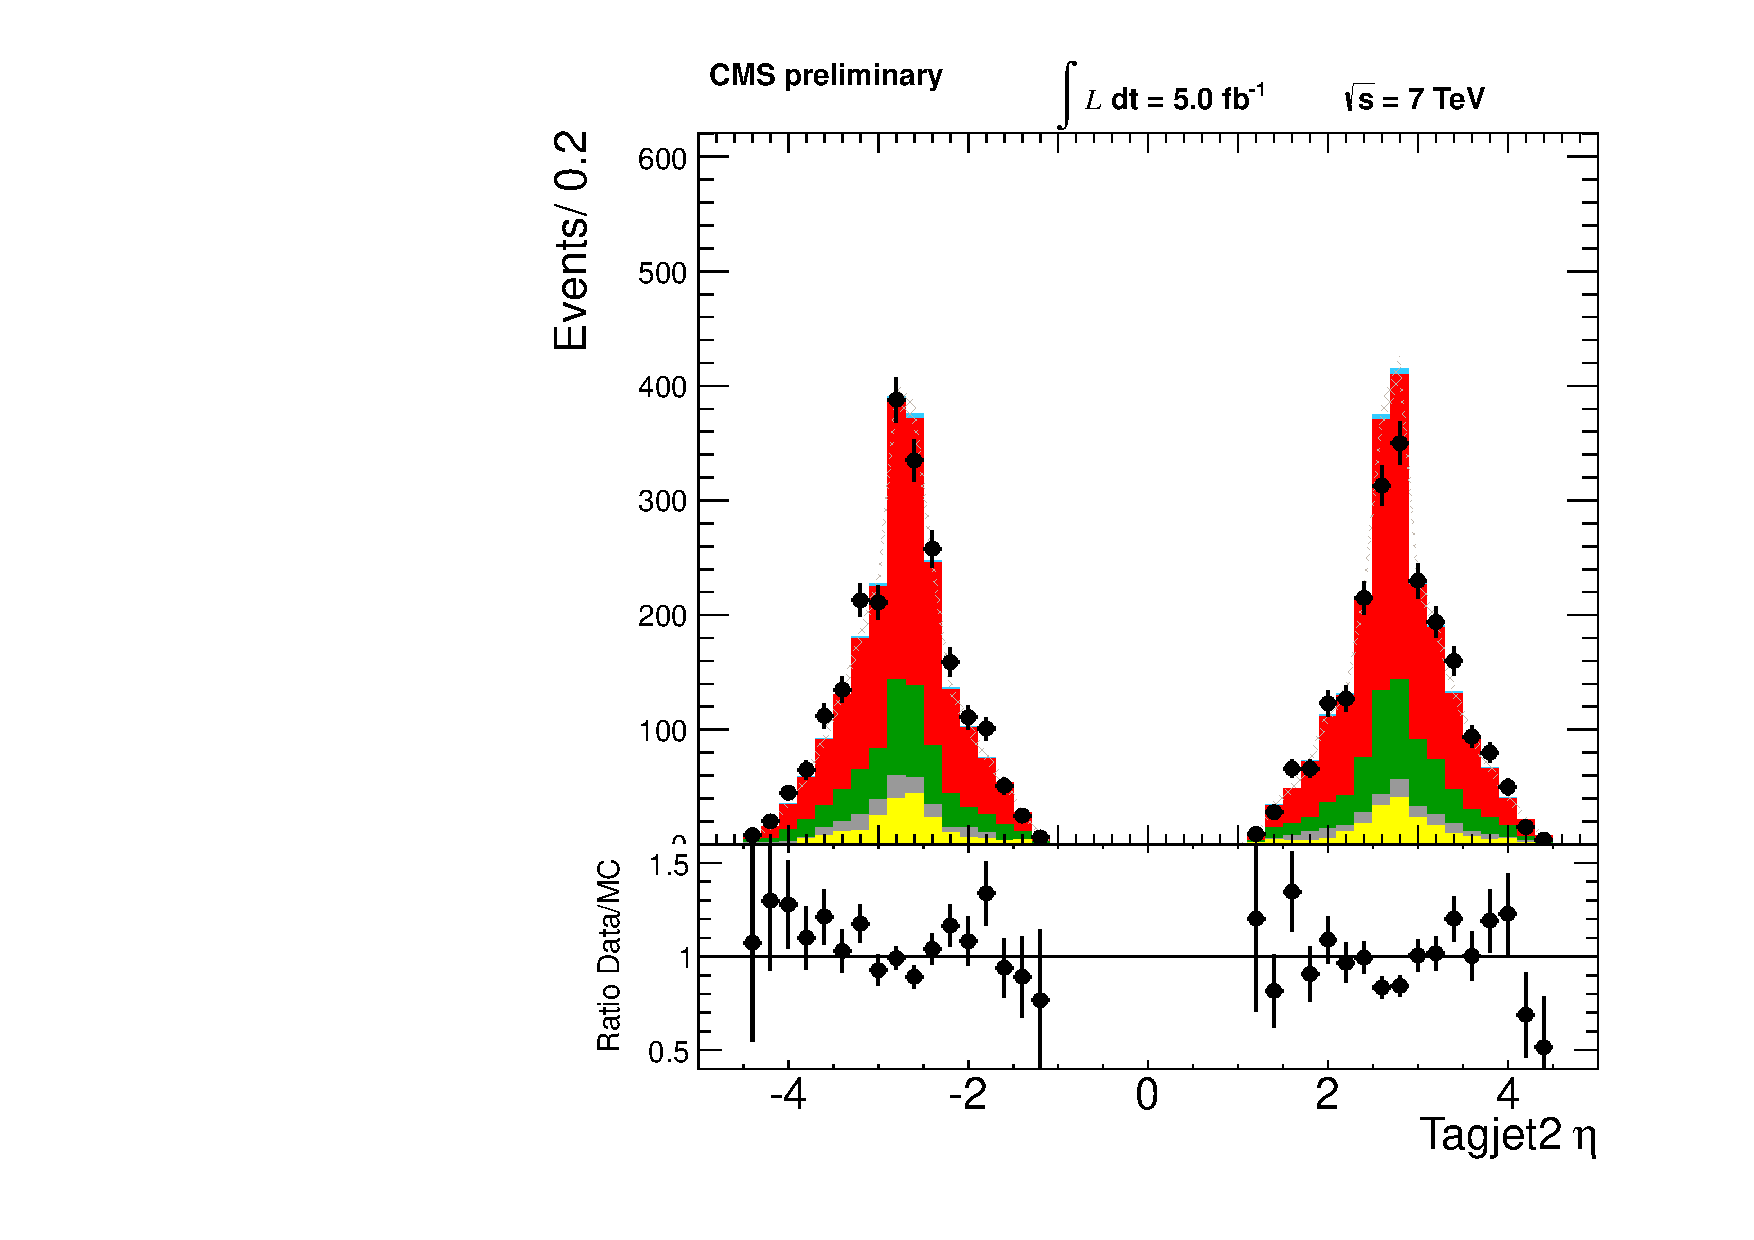
\includegraphics[width=0.49\textwidth]{figs/n-1_plots_el/el_vbftagjetb_eta.pdf}
    \caption{Comparison of the first (left) and second (right)
      VBF-tagged jet $\eta $ distributions from data and MC for the
      electron+jets selection.  }
\label{fig:el_tagjet_eta}}
\end{figure}

%%%%%%%%%%%%%%%%%%%%%%%%%%%%
\begin{figure}[h!t]
  {\centering
    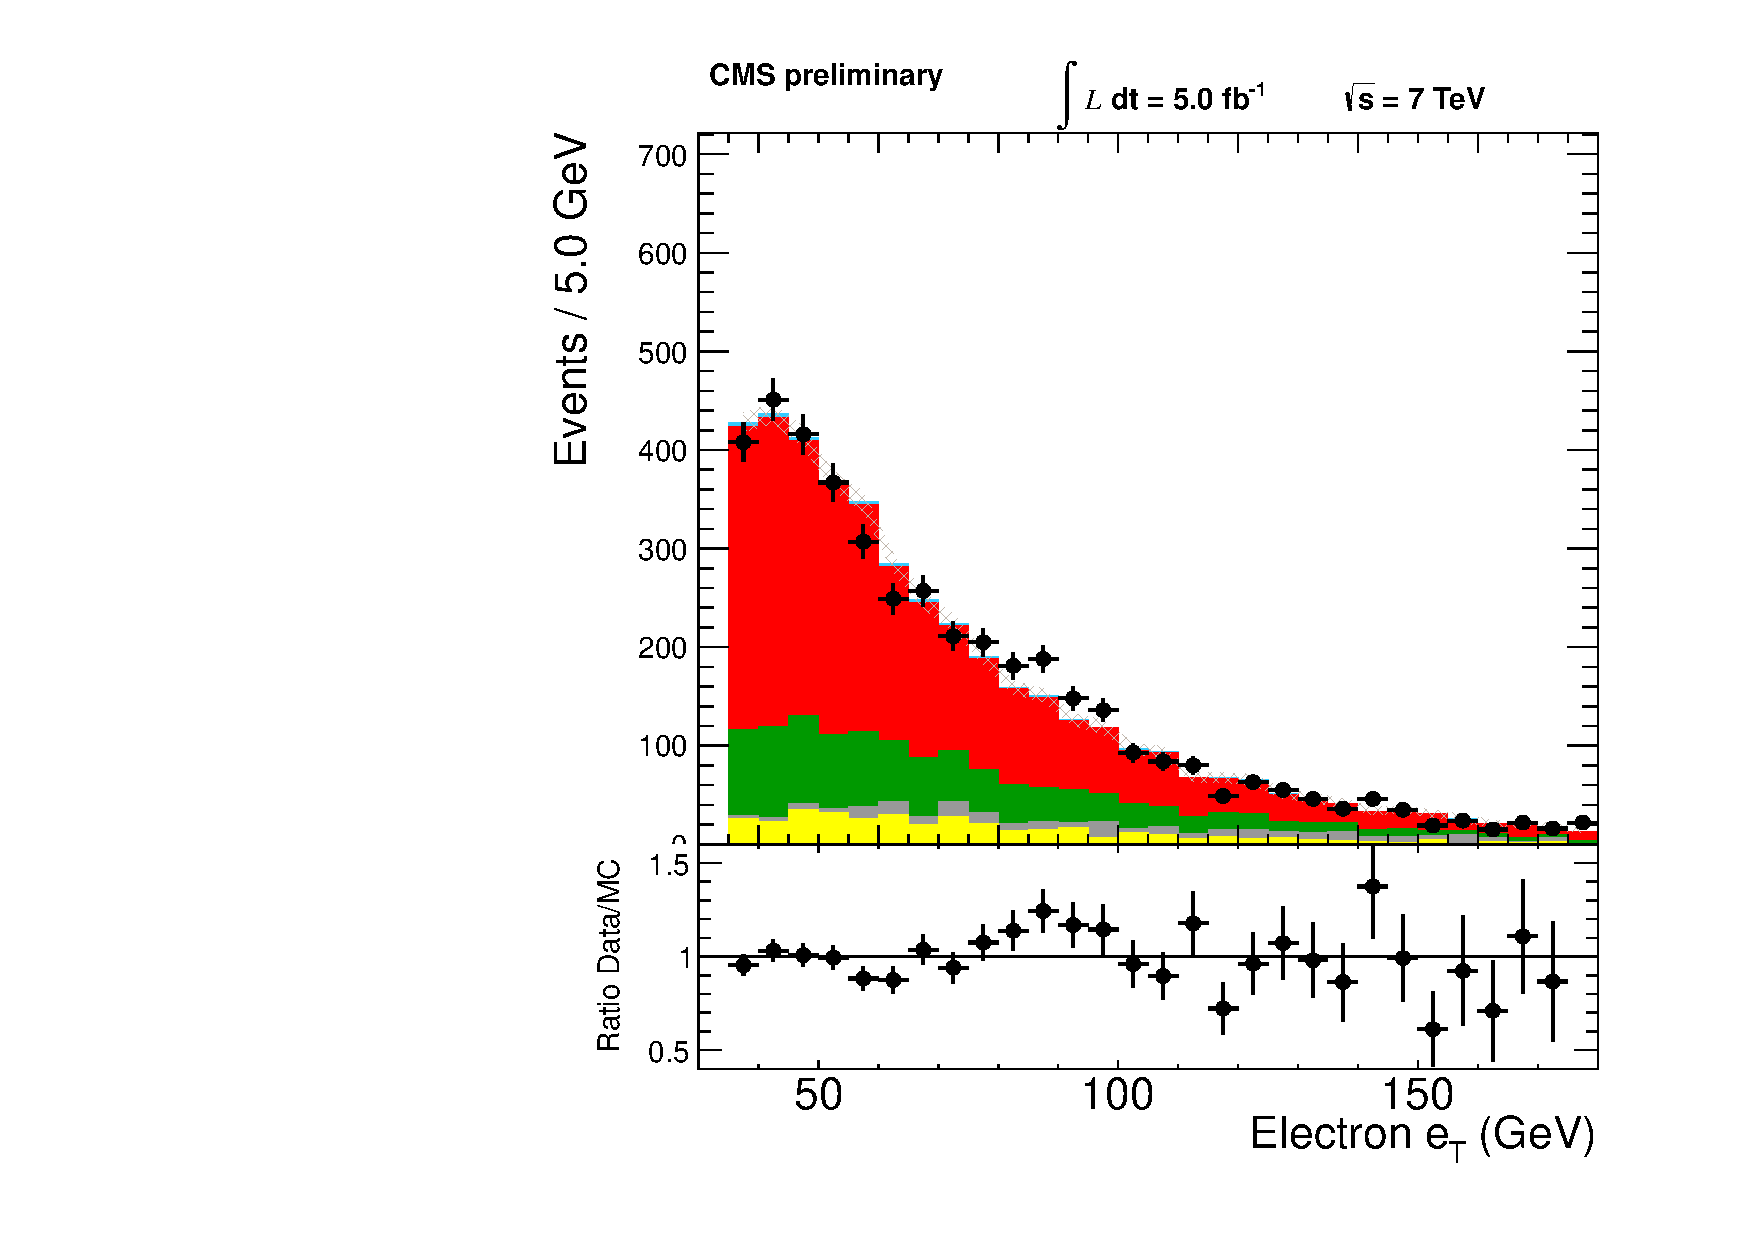
\includegraphics[width=0.49\textwidth]{figs/n-1_plots_el/el_W_electron_et.pdf}
    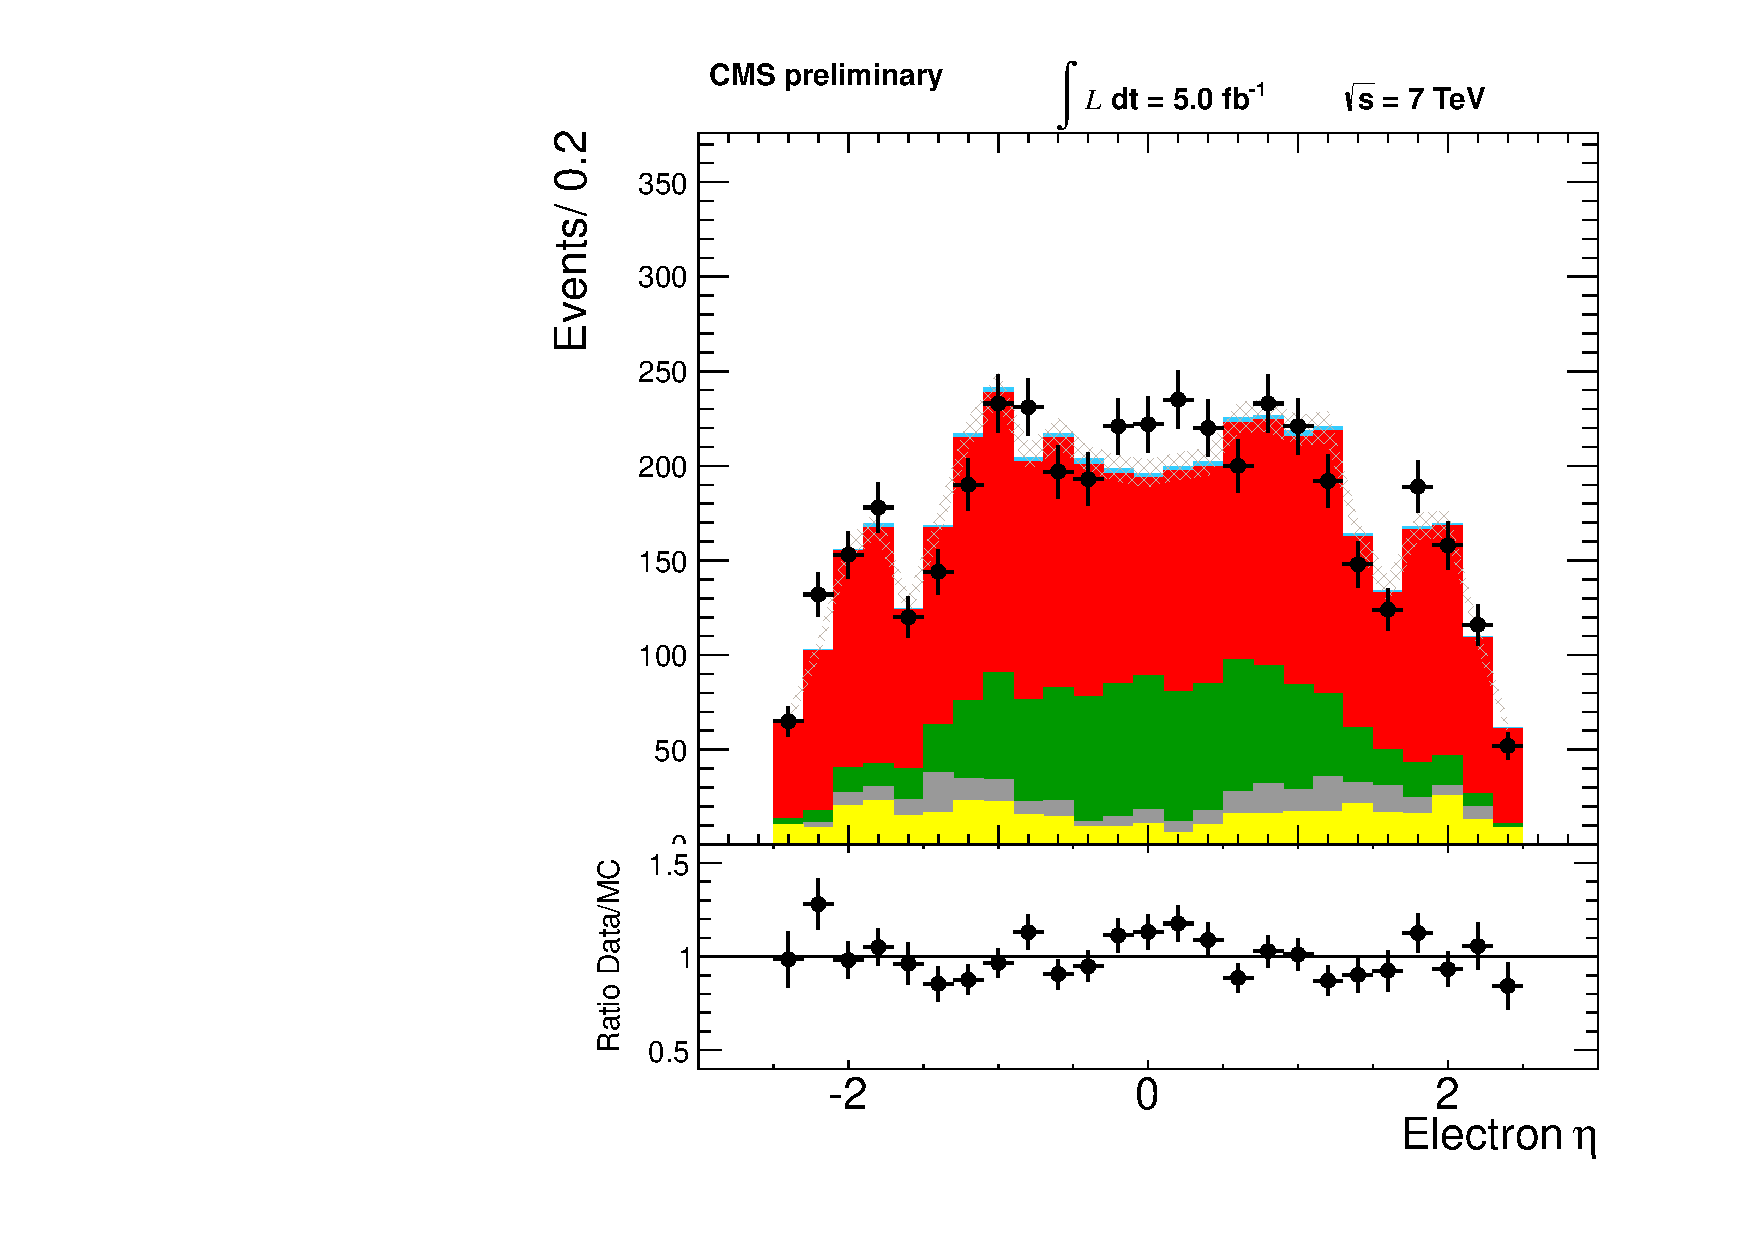
\includegraphics[width=0.49\textwidth]{figs/n-1_plots_el/el_W_electron_eta.pdf}
    \caption{Comparison of the electron $E_{T} $ (left) and the
    electron $\eta $ (right) distributions from data and MC for the
    electron+jets selection. 
    }
   \label{fig:el_electron}}
\end{figure}
%%%%%%%%%%%%%%%%%%%%%%%%%%%%
\begin{figure}[h!t]
  {\centering
    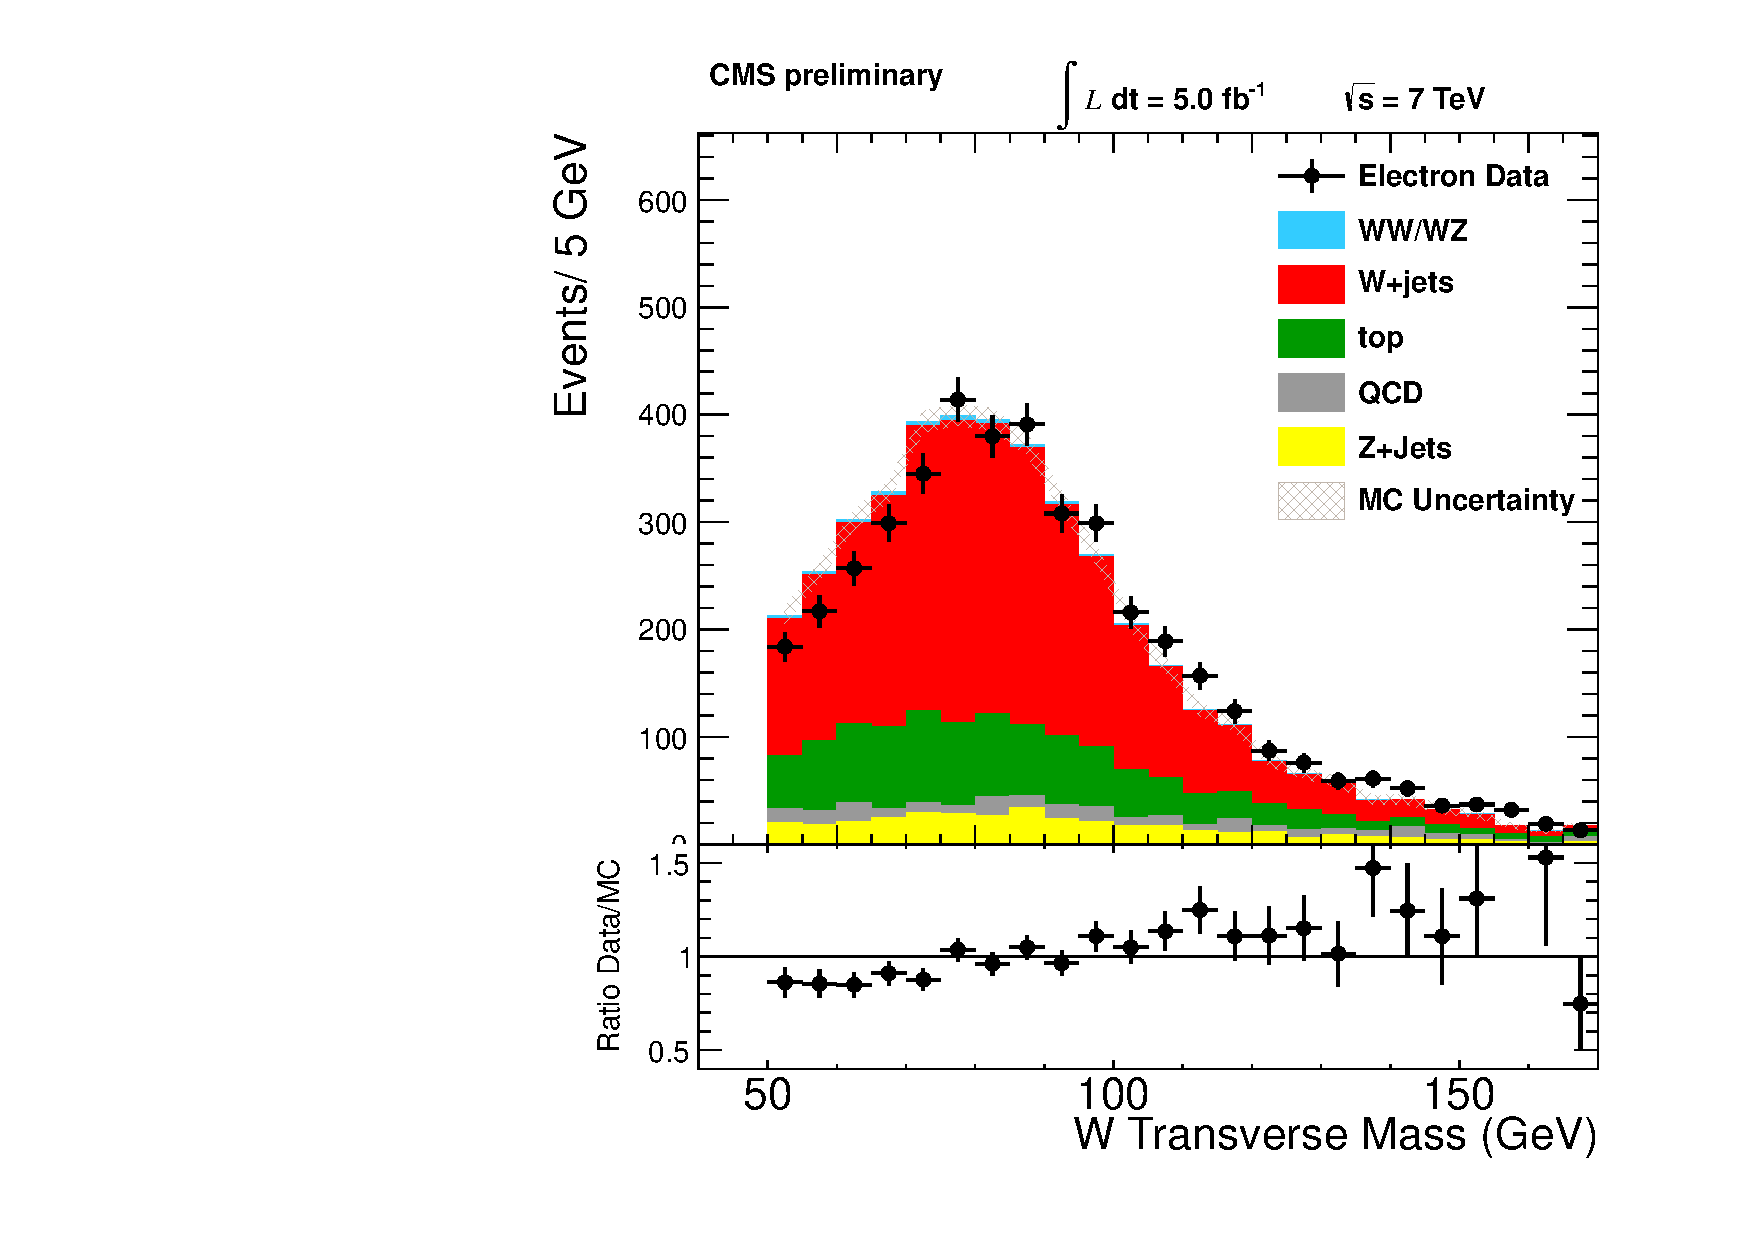
\includegraphics[width=0.49\textwidth]{figs/n-1_plots_el/el_vbf_W_mt.pdf}
    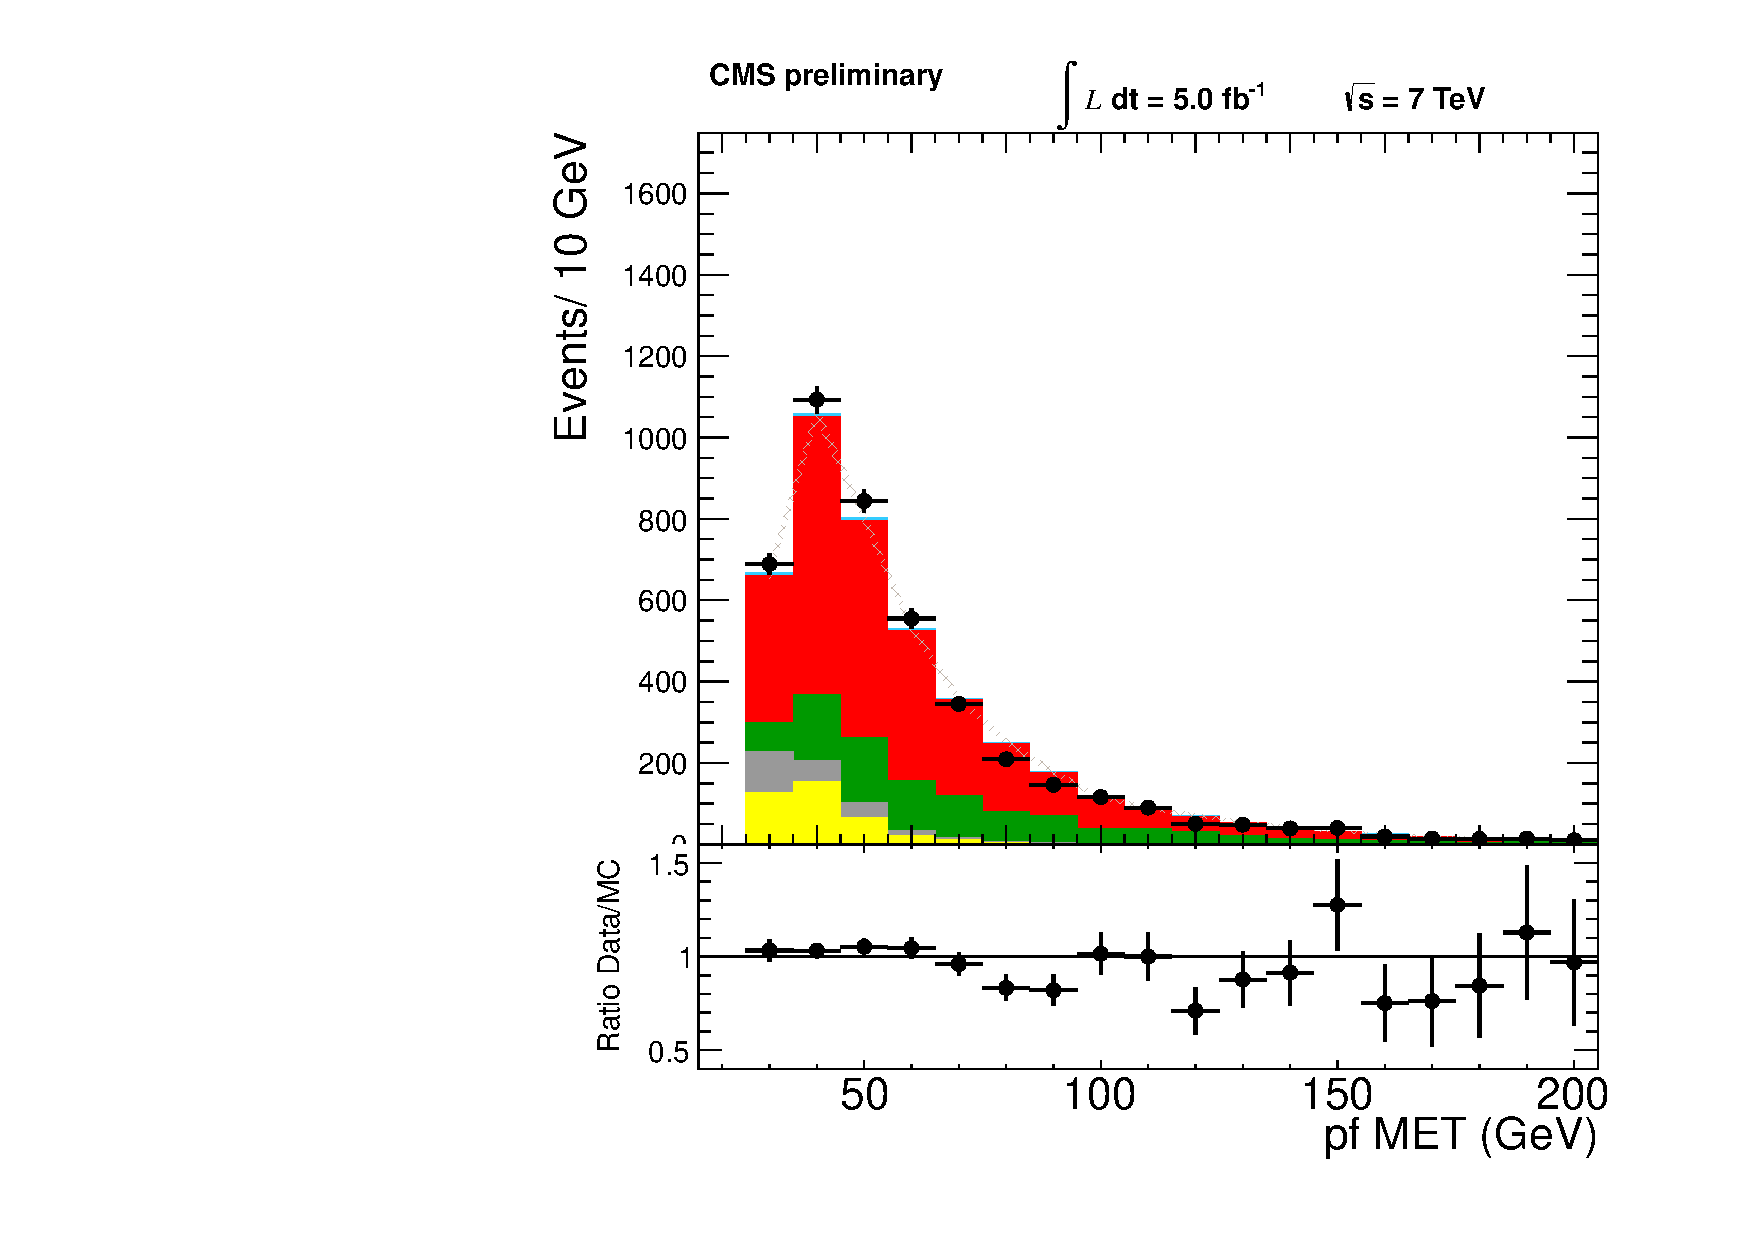
\includegraphics[width=0.49\textwidth]{figs/n-1_plots_el/el_event_met_pfmet.pdf}
    \caption{Comparison of the distributions from data and MC of the transverse mass
     of electron / MET system (left) and the MET (right) for the
      electron+jets selection. 
      }
    \label{fig:el_W_Mt}}
\end{figure}
%%%%%%%%%%%%%%%%%%%%%%%%%%%%
\begin{figure}[h!t]
  {\centering
    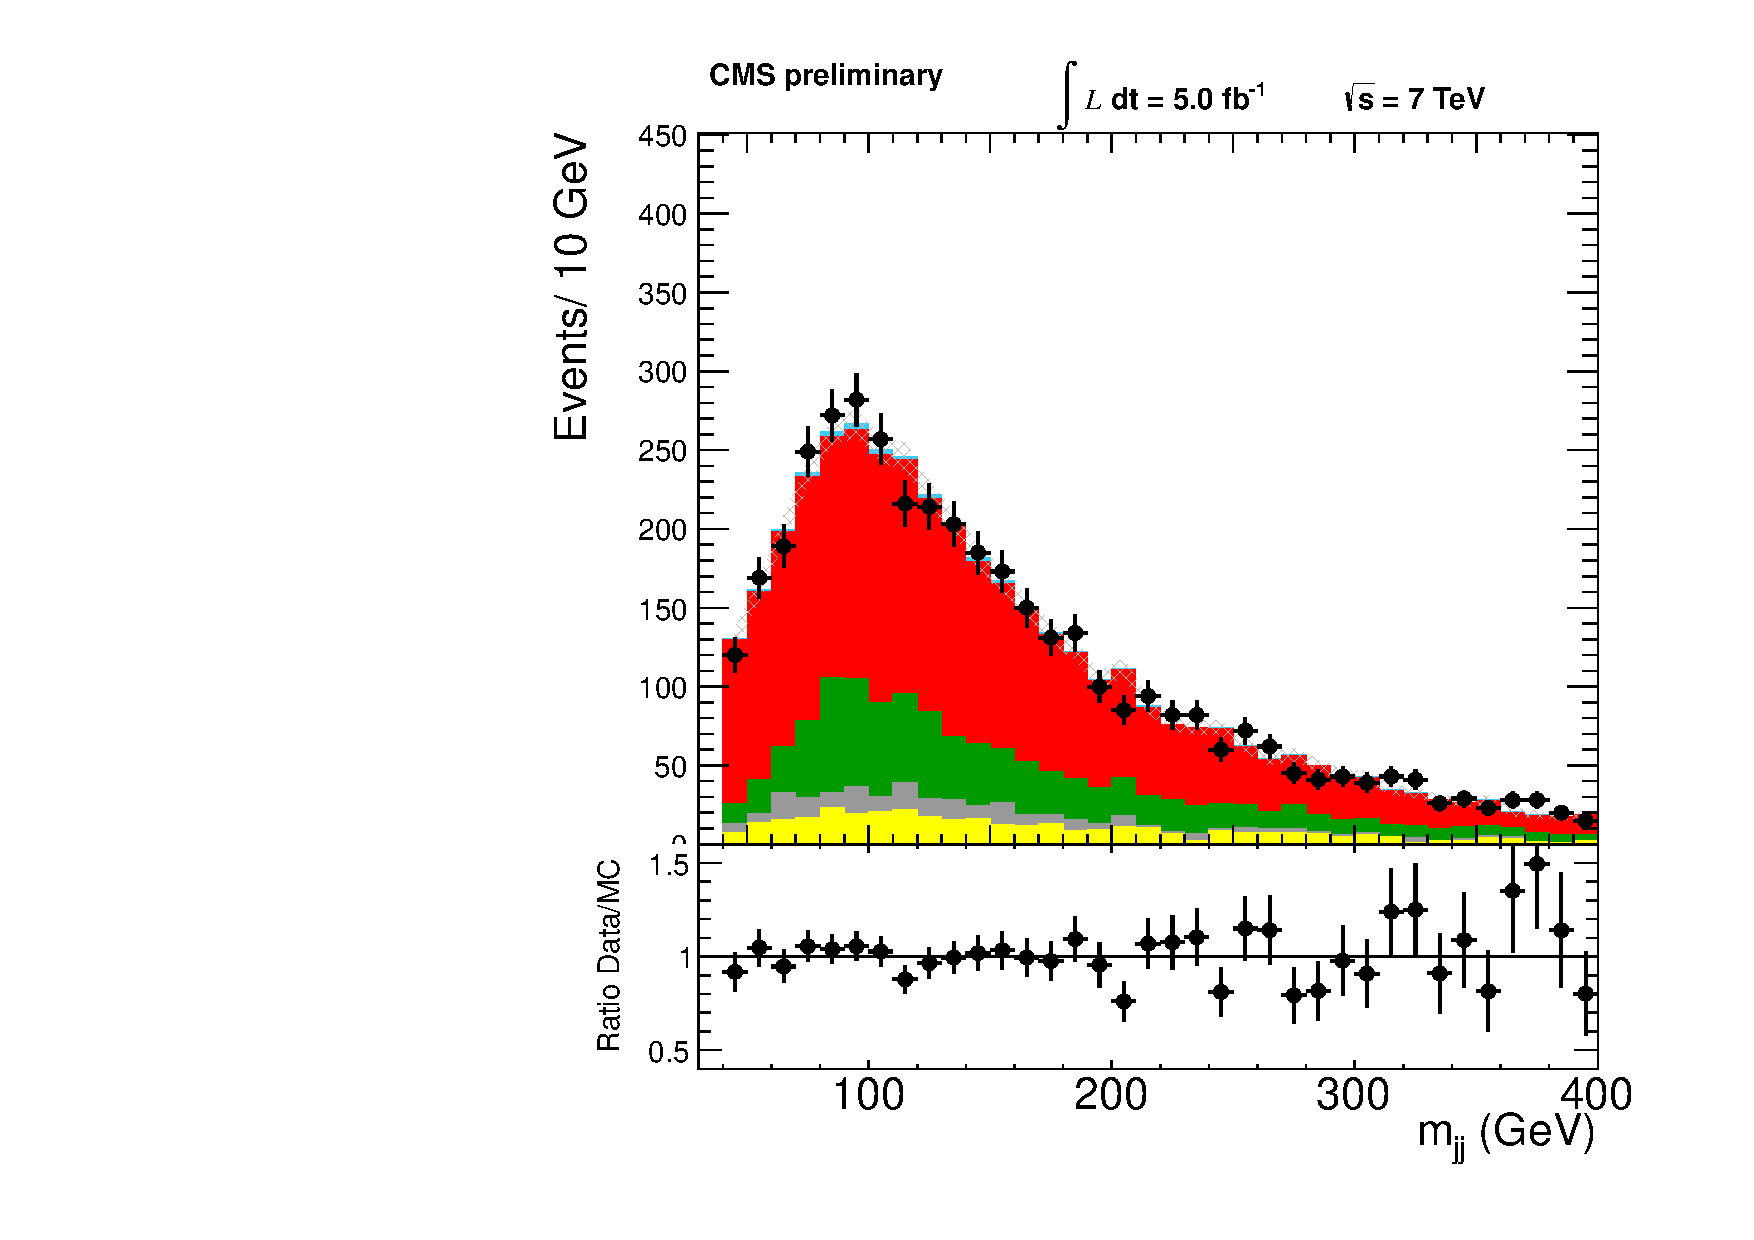
\includegraphics[width=0.49\textwidth]{figs/n-1_plots_el/el_vbfwjjmass.pdf}
    \caption{Comparison of the hadronic W dijet mass ($m_{JJ}$)
      distributions from data and MC for the electron+jets
      selection. }
    \label{fig:el_mjj}}
\end{figure}

%%%%%%%%%%%%%%%%%%%%%%%%%%%%
%%%%%%%%%%%%%%%%%%%%%%%%%%%%
\clearpage
The data MC comparison for the various inputs to the MVA are shown in  
Figures ~\ref{fig:mu_theta}-\ref{fig:mu_tagjet_pair}
for the muon+jets sample and in 
Figures ~\ref{fig:el_theta}-\ref{fig:el_tagjet_pair} for
the electron+jets sample. 

% angular variables
%%%%%%%%%%%%%%%%%%%%%%%%%%%%
\begin{figure}[h!t]
  {\centering
    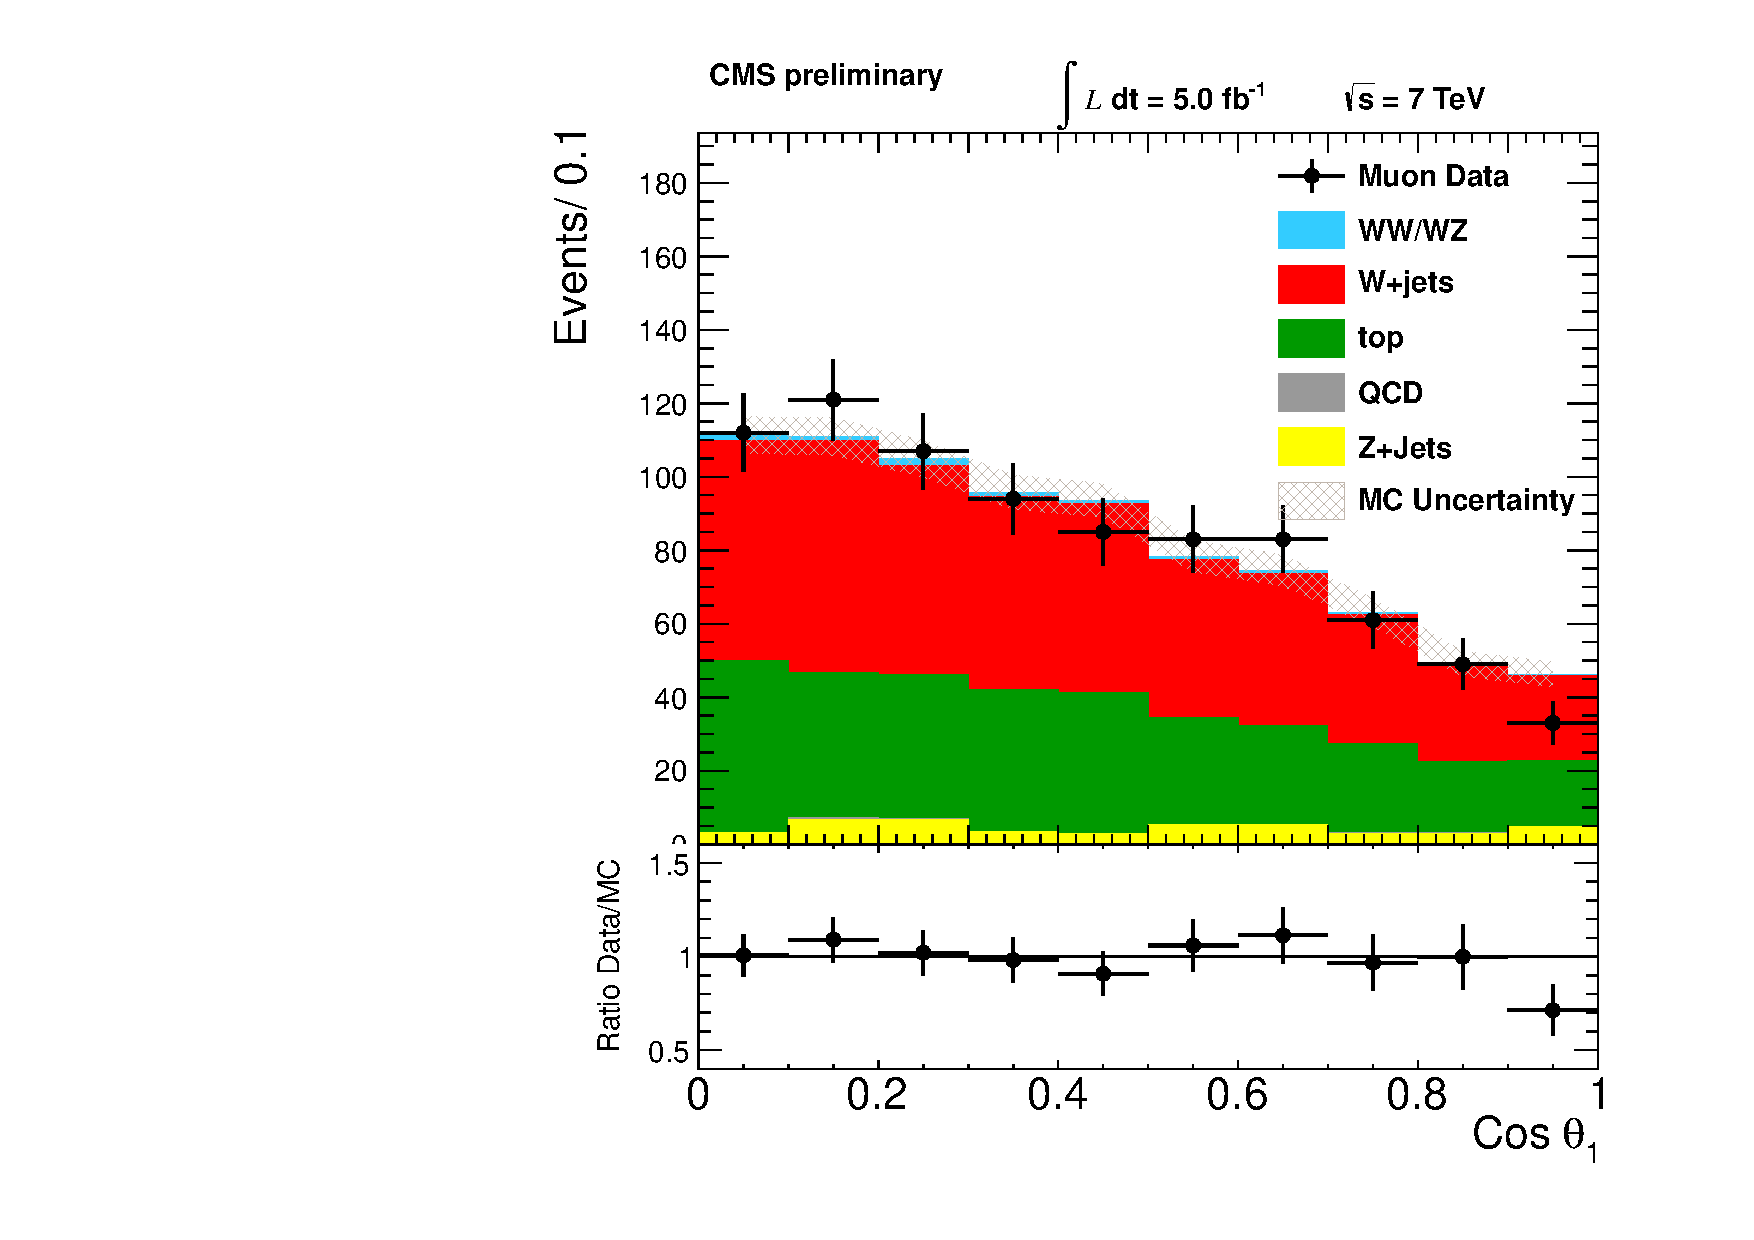
\includegraphics[width=0.49\textwidth]{figs/n-1_plots_mu/mu_vbfangha.pdf}
    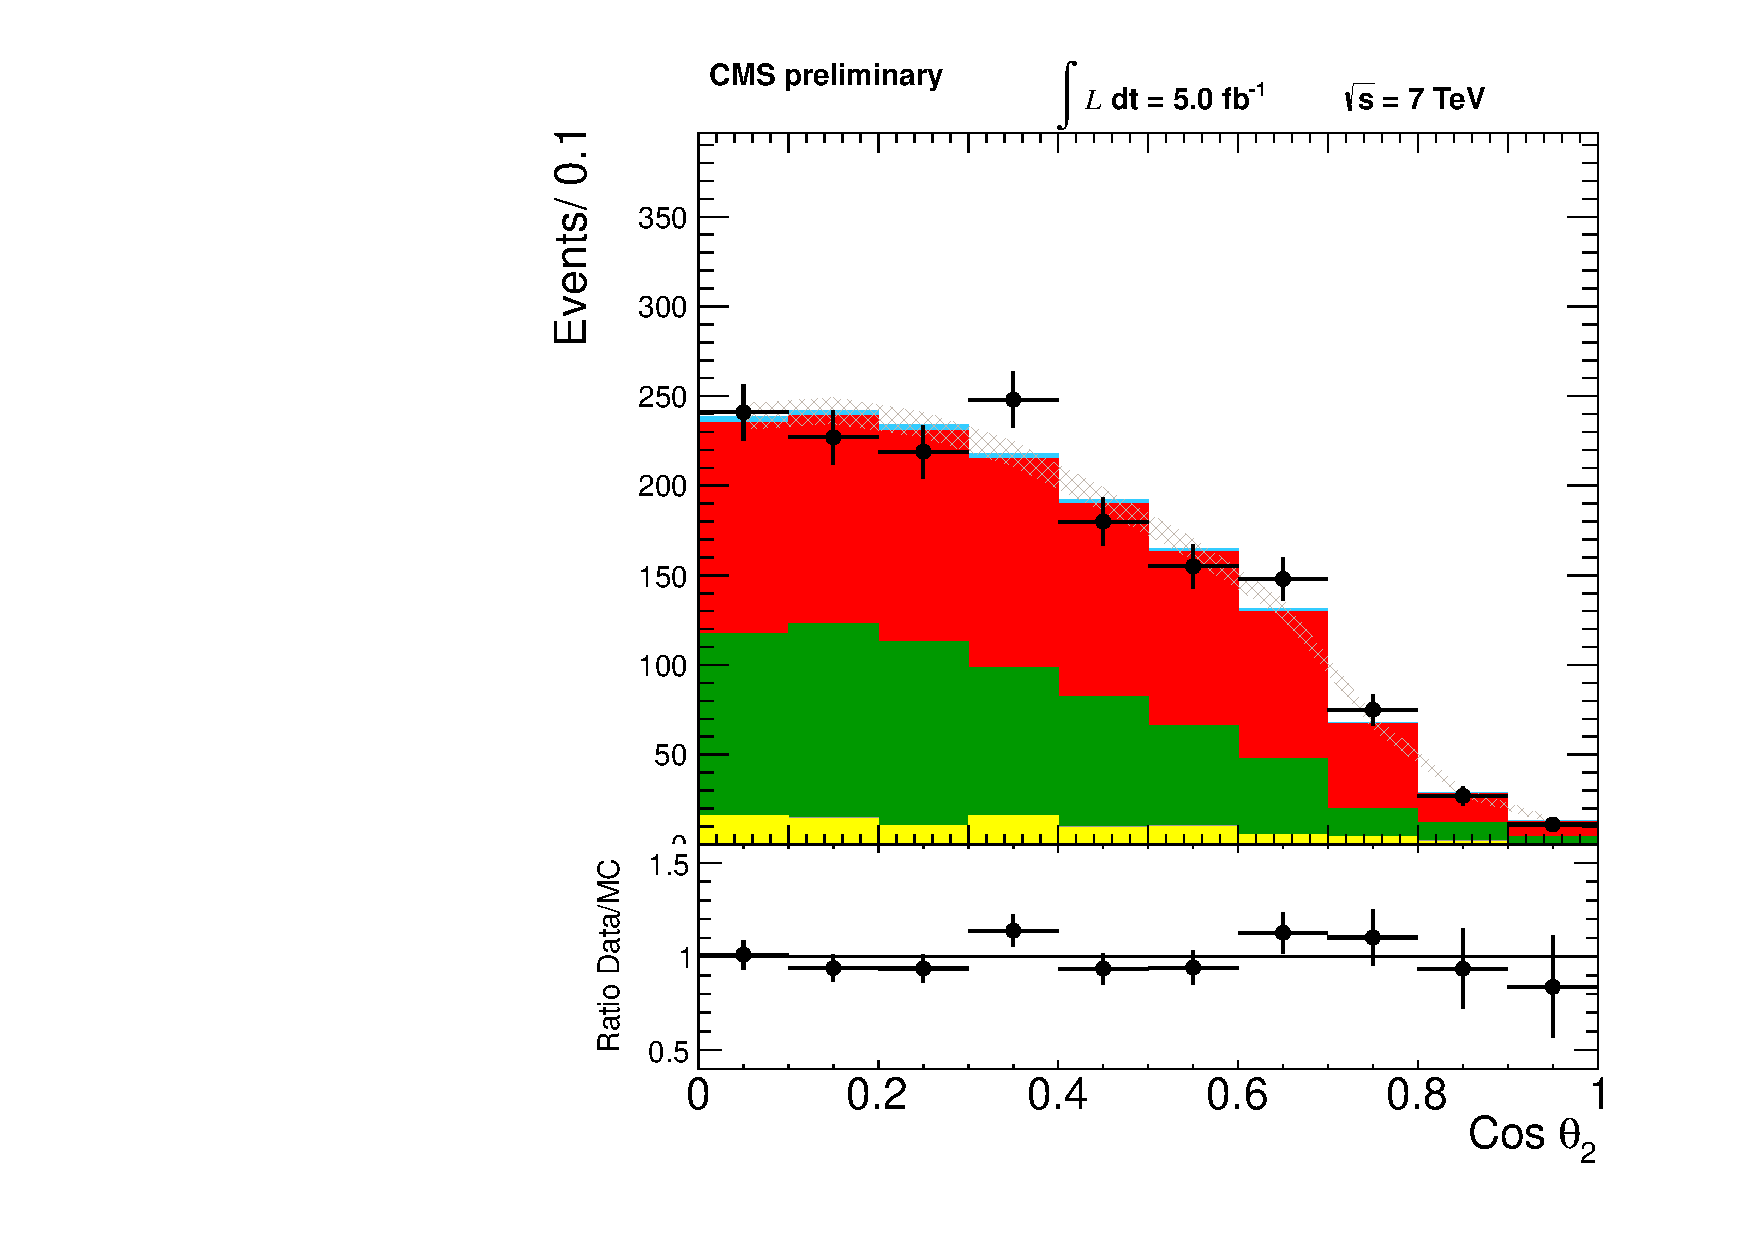
\includegraphics[width=0.49\textwidth]{figs/n-1_plots_mu/mu_vbfanghb.pdf}
    \caption{Comparison of the angular distributions for $\cos\theta_{1}$ (left)
   $\cos\theta_{2}$ (right) from data and MC for the muon+jets selection.}
\label{fig:mu_theta}}
\end{figure}
%%%%%%%%%%%%%%%%%%%%%%%%%%%%
\begin{figure}[h!t]
  {\centering
     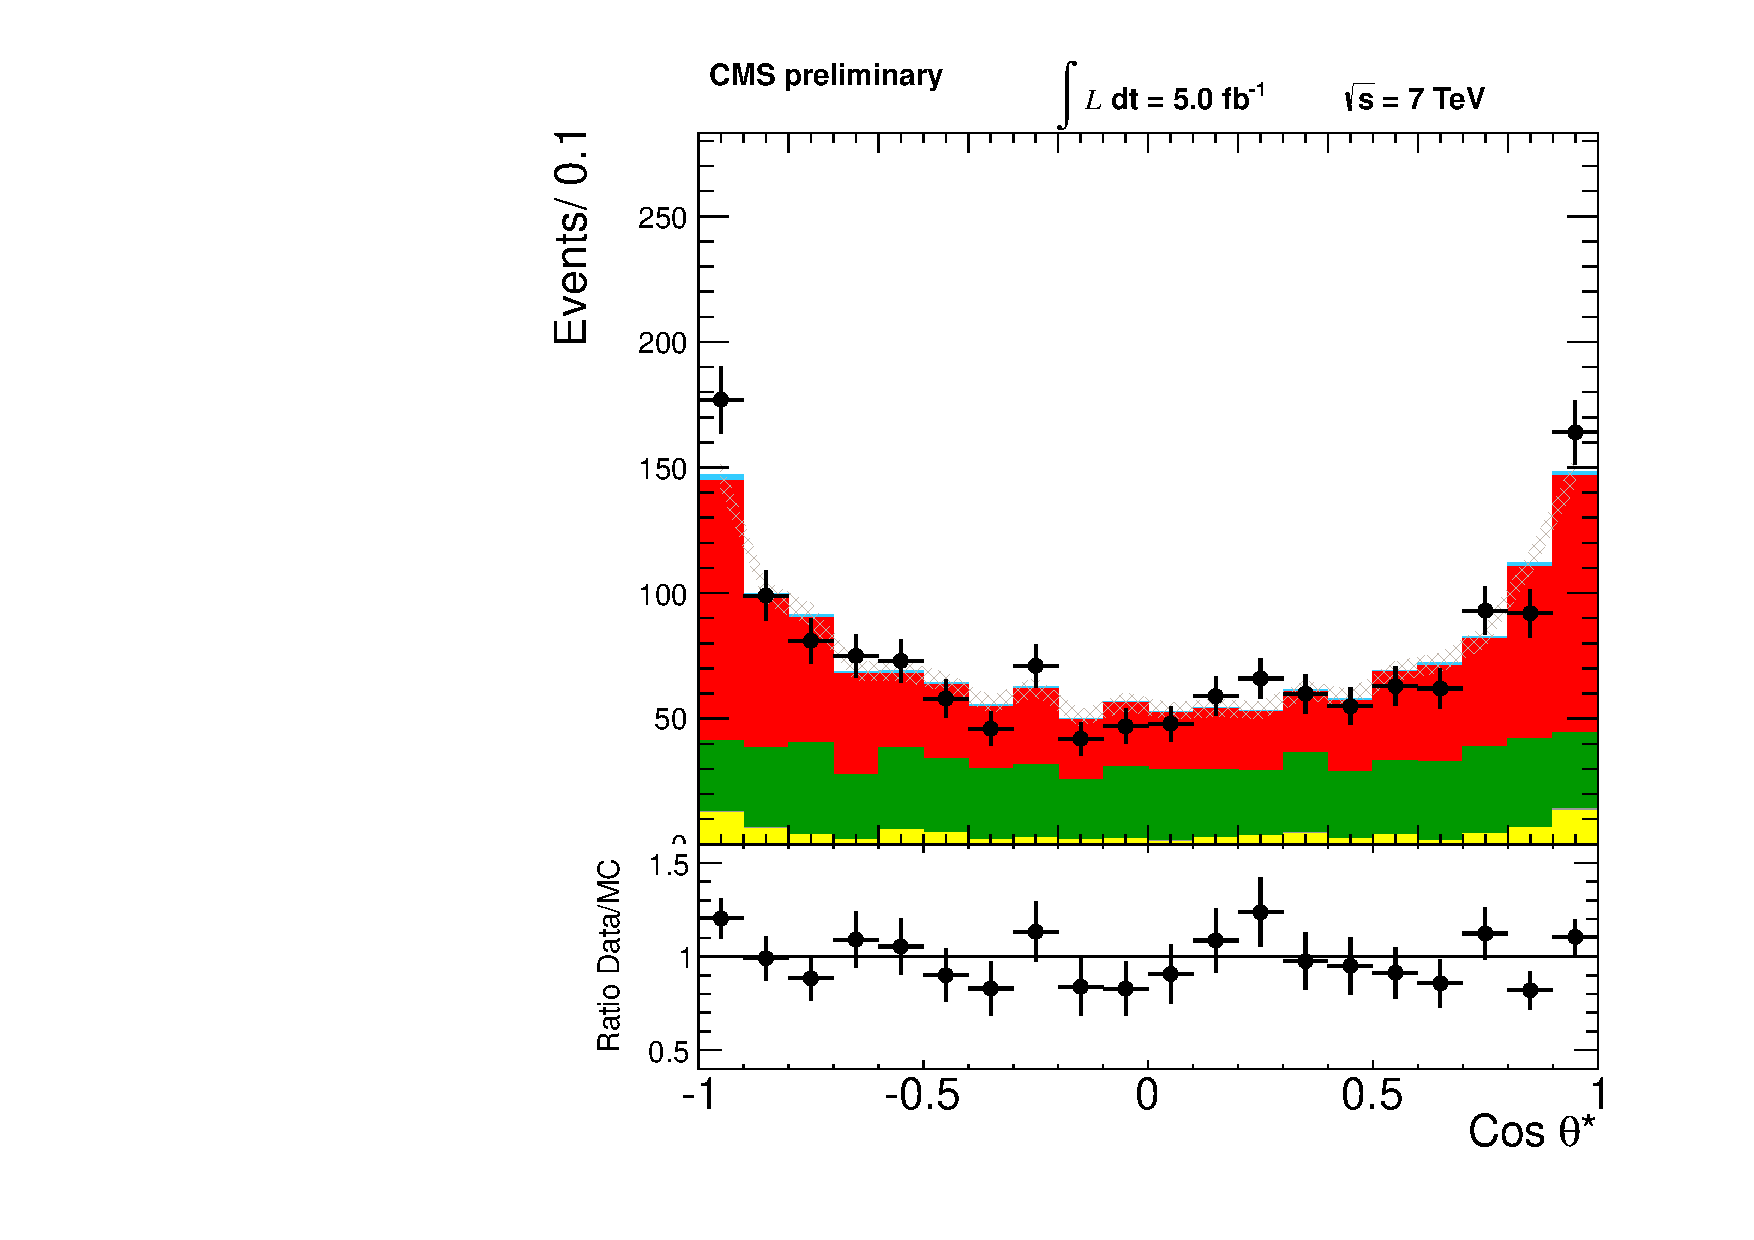
\includegraphics[width=0.49\textwidth]{figs/n-1_plots_mu/mu_vbfanghs.pdf}
    \caption{Comparison of the angular distributions for $\cos\theta^{\ast}$ from data and MC 
   for the muon+jets selection.}
\label{fig:mu_thetas}}
\end{figure}
%%%%%%%%%%%%%%%%%%%%%%%%%%%%
\begin{figure}[h!t]
  {\centering
    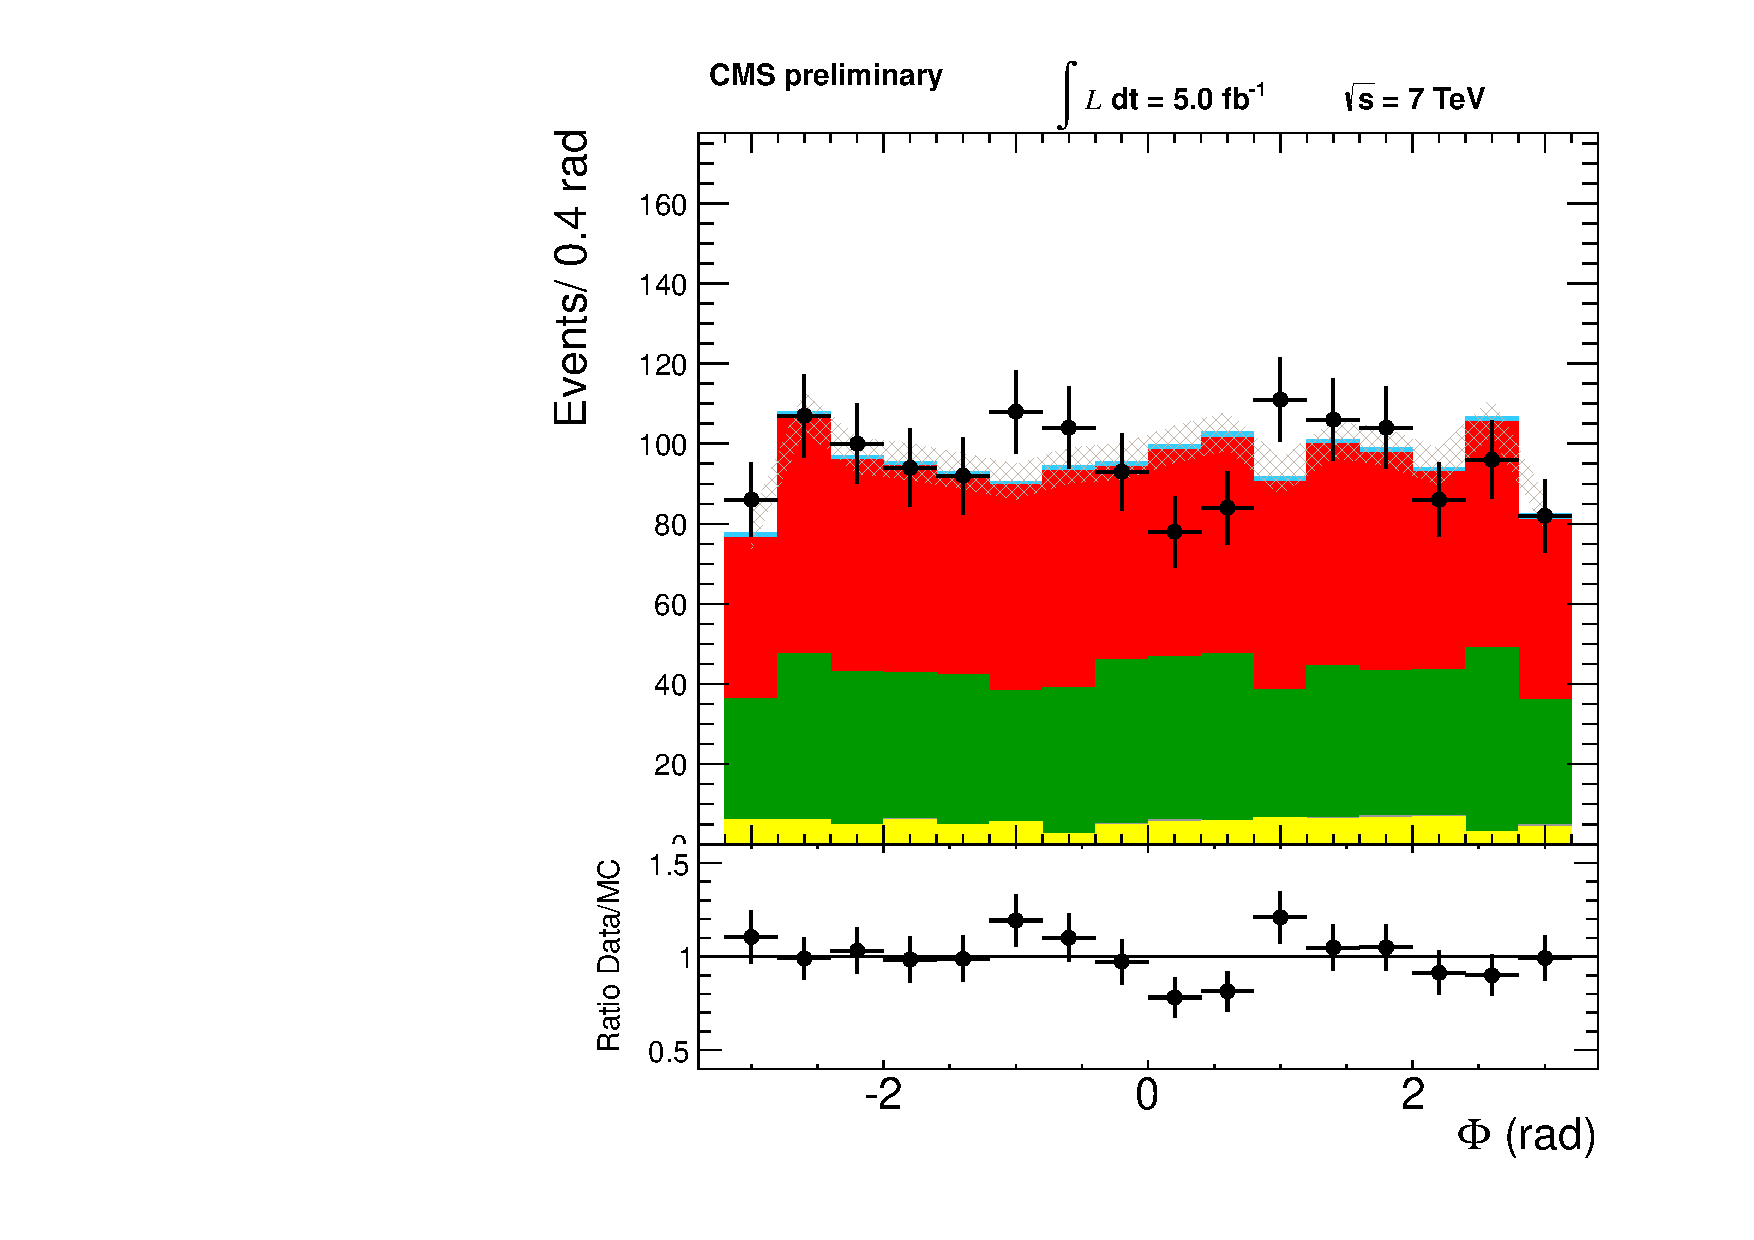
\includegraphics[width=0.49\textwidth]{figs/n-1_plots_mu/mu_vbfangphi.pdf}
    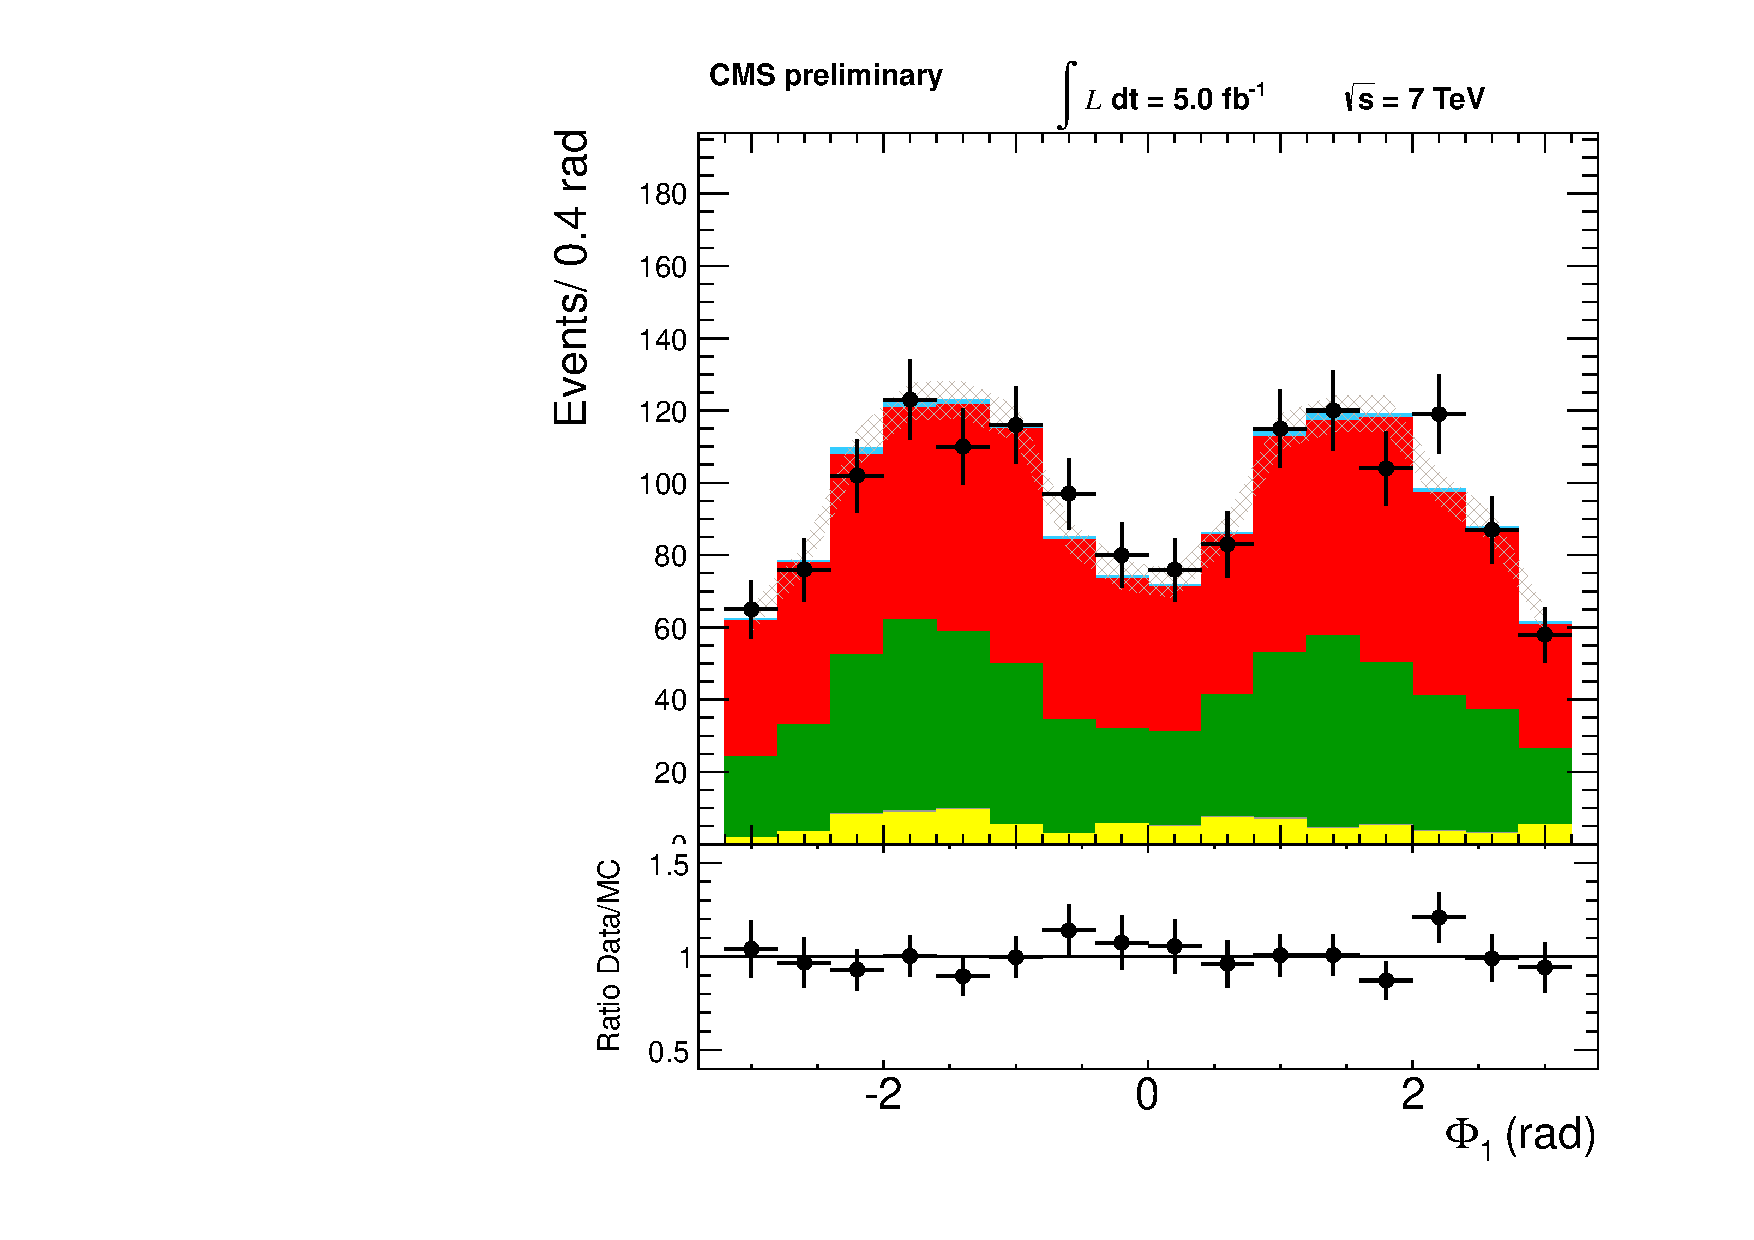
\includegraphics[width=0.49\textwidth]{figs/n-1_plots_mu/mu_vbfangphib.pdf}
    \caption{Comparison of the angular distributions for $\Phi$  (left)$\Phi_{1}$ (right) from data and 
      MC for the muon+jets selection.}
\label{fig:mu_phi}}
\end{figure}

%%%%%%%%%%%%%%%%%%%%%%%%%%%%
\begin{figure}[h!t]
  {\centering
    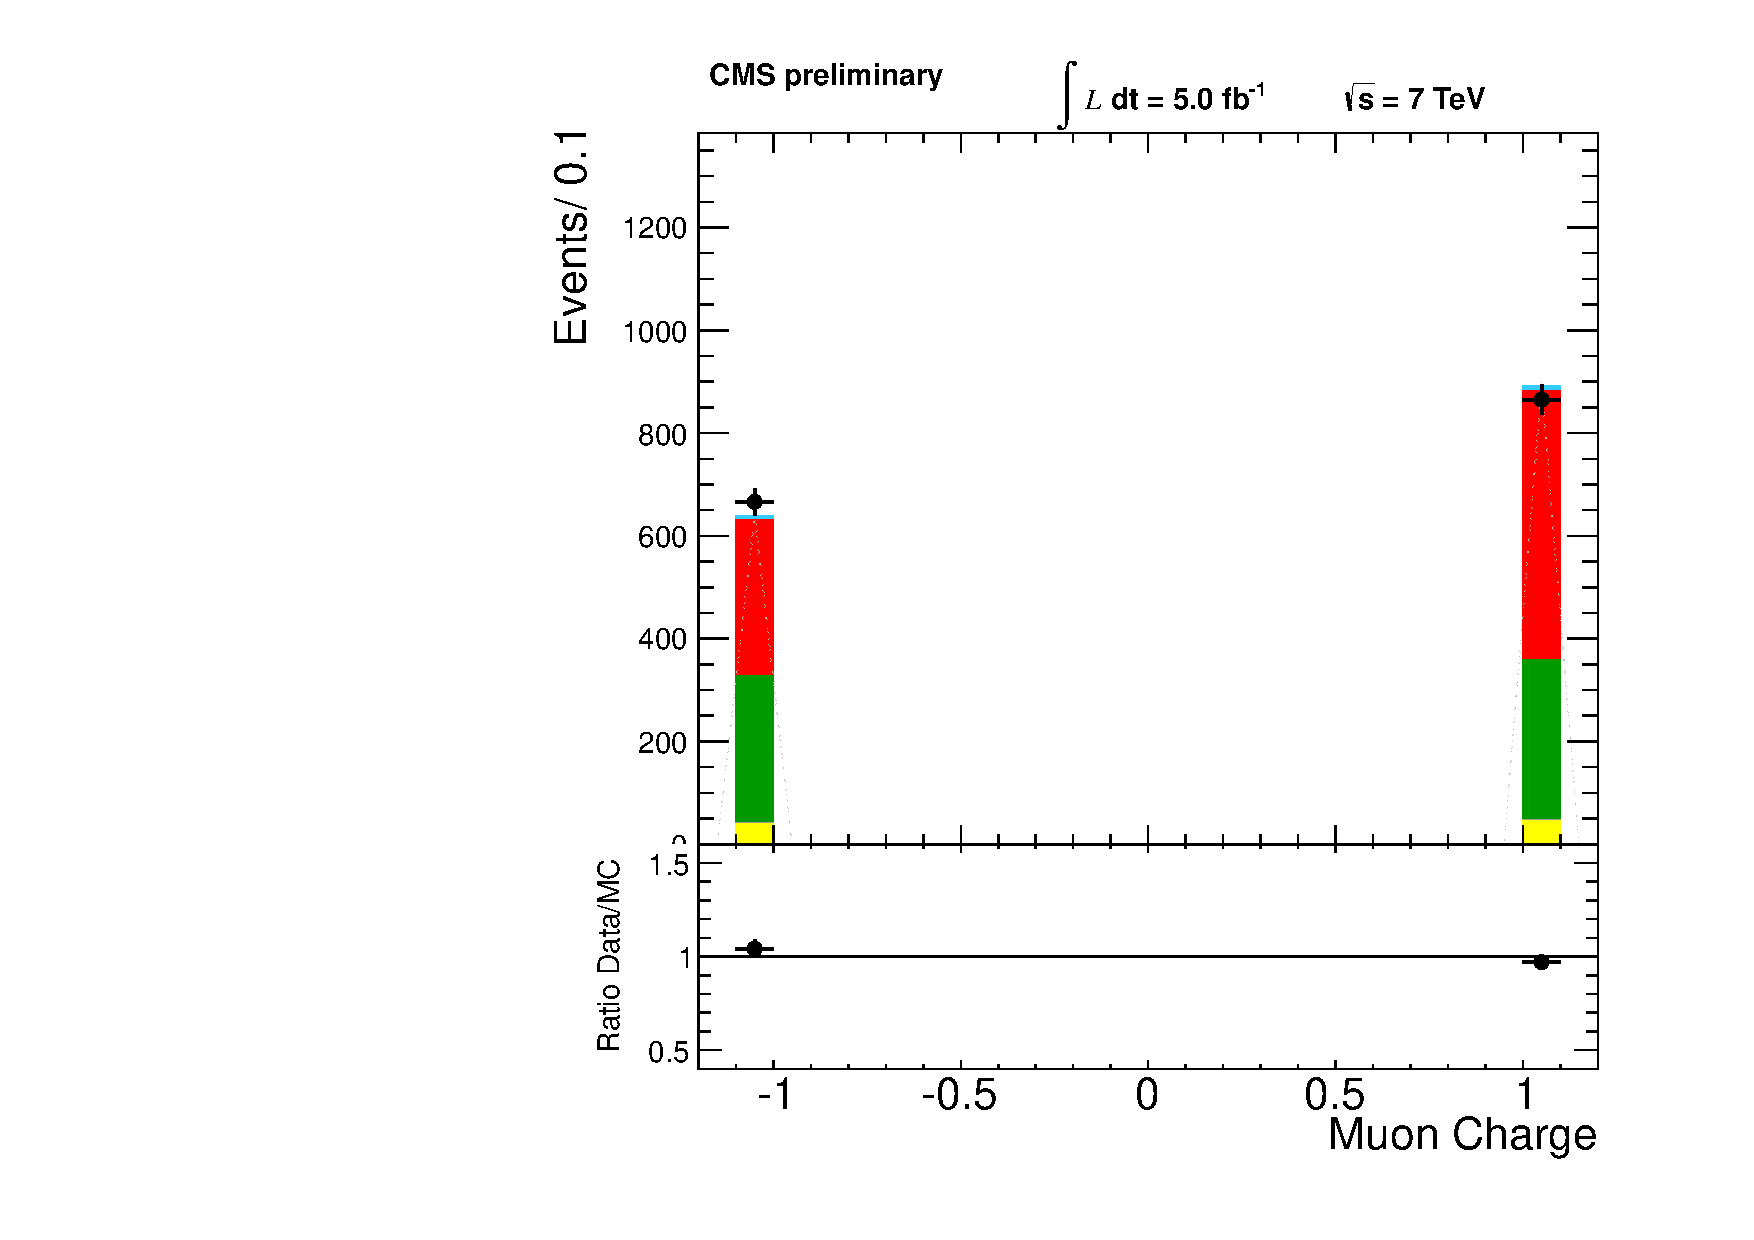
\includegraphics[width=0.49\textwidth]{figs/n-1_plots_mu/mu_vbfWmucharge.pdf}
    \caption{Comparison of the charge of the muon from data and MC for the muon+jets selection.}
\label{fig:mu_chg}}
\end{figure}

% rapidity and pt of the WW system

%%%%%%%%%%%%%%%%%%%%%%%%%%%%
\begin{figure}[h!t]
  {\centering
    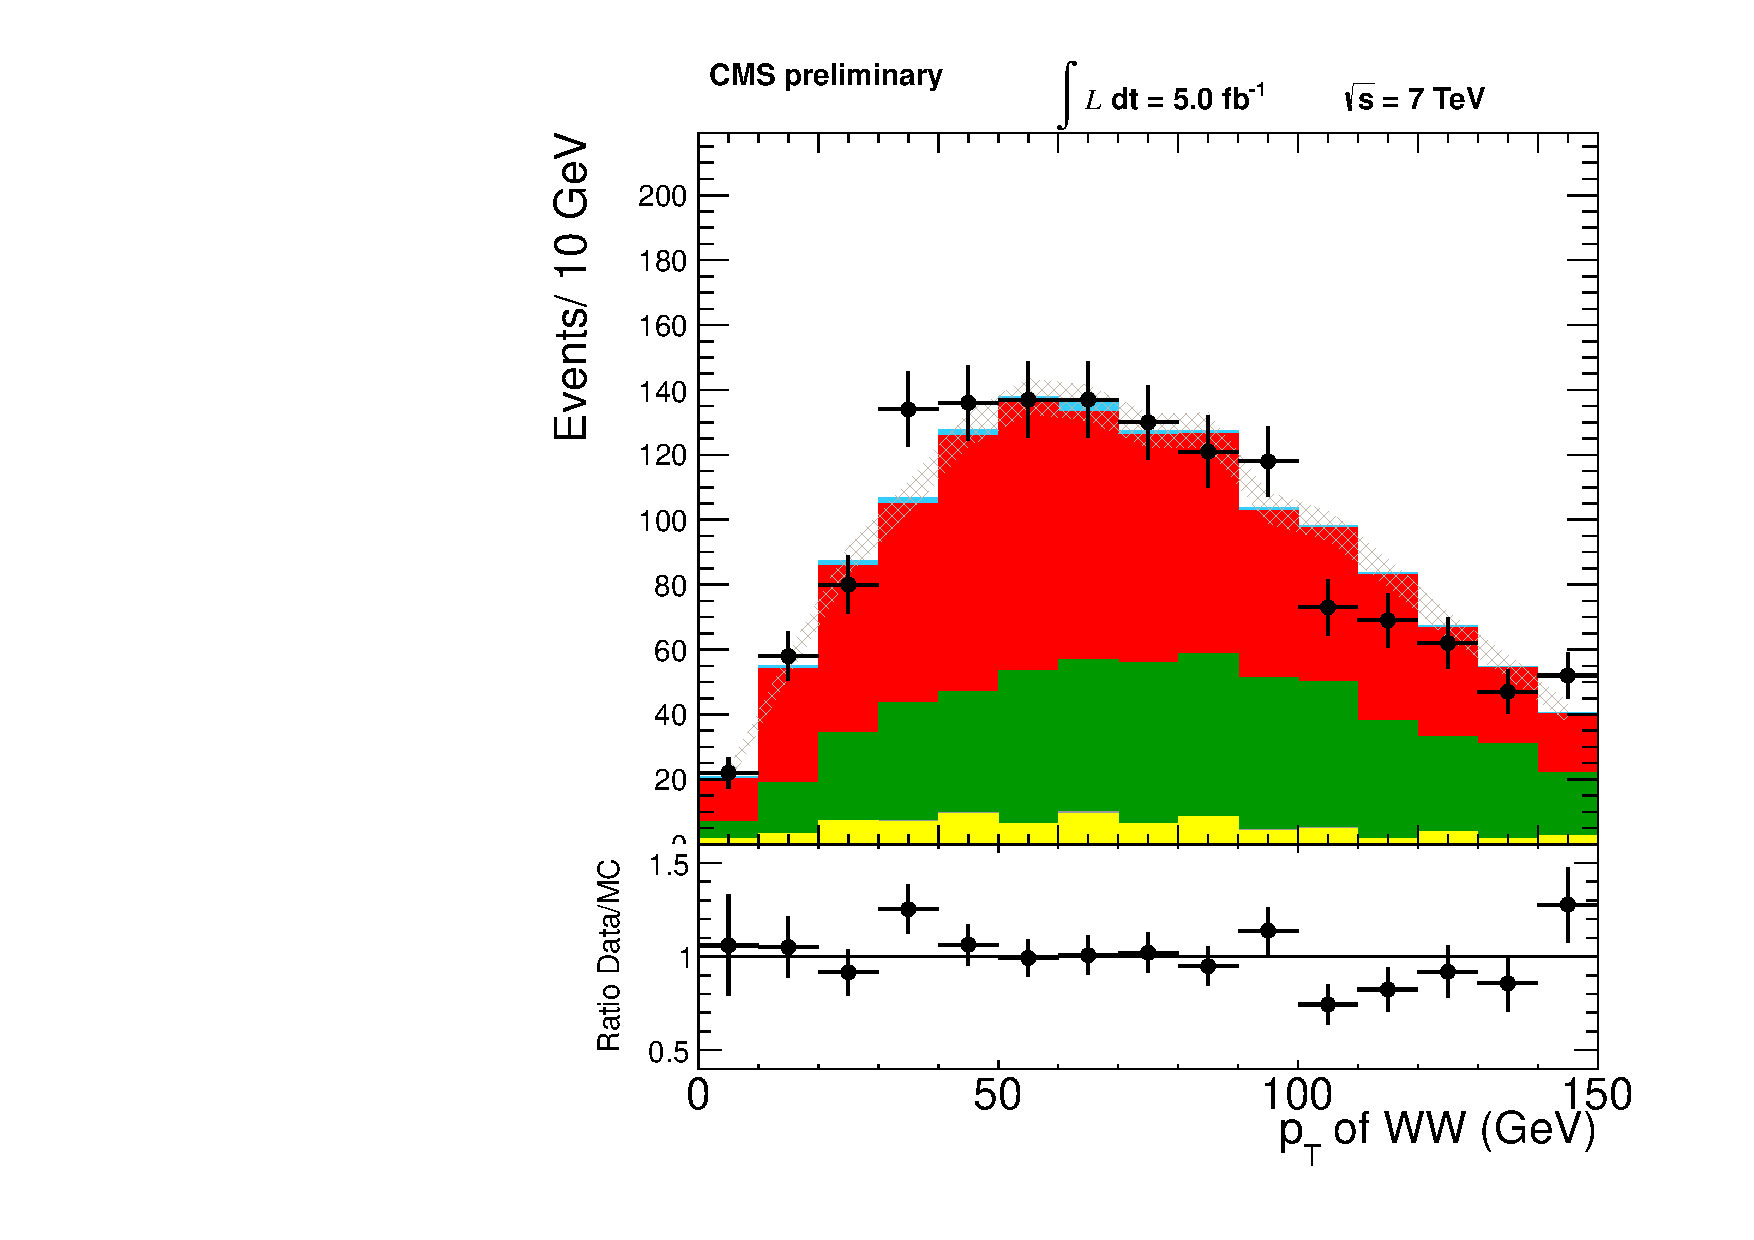
\includegraphics[width=0.49\textwidth]{figs/n-1_plots_mu/mu_vbfptlvjj.pdf}
    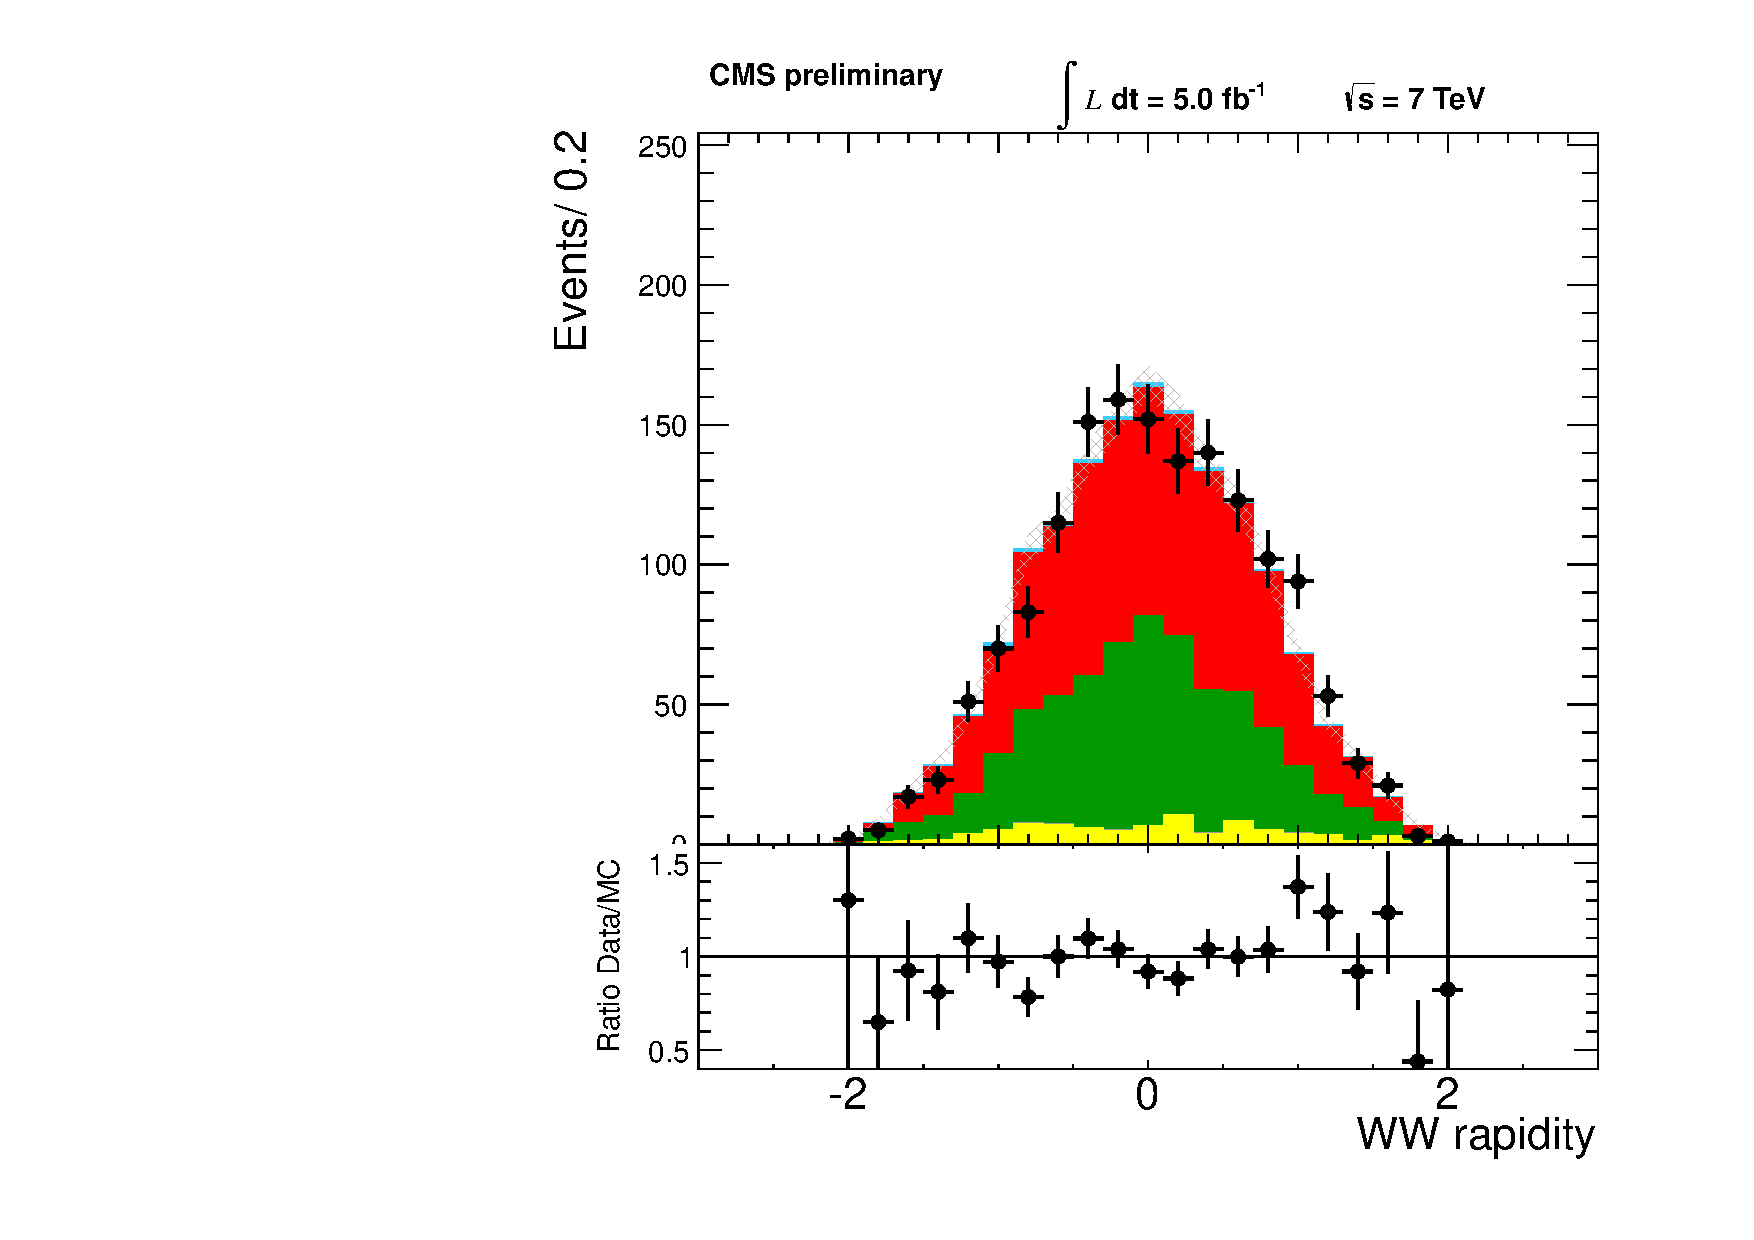
\includegraphics[width=0.49\textwidth]{figs/n-1_plots_mu/mu_vbfetalvjj.pdf}
    \caption{Comparison of the $p_{T}$ (left) $\eta$ (right) of the WW system
      from data and MC for the muon+jets selection.}
\label{fig:mu_ww}}
\end{figure}

\begin{figure}[h!t]
  {\centering
    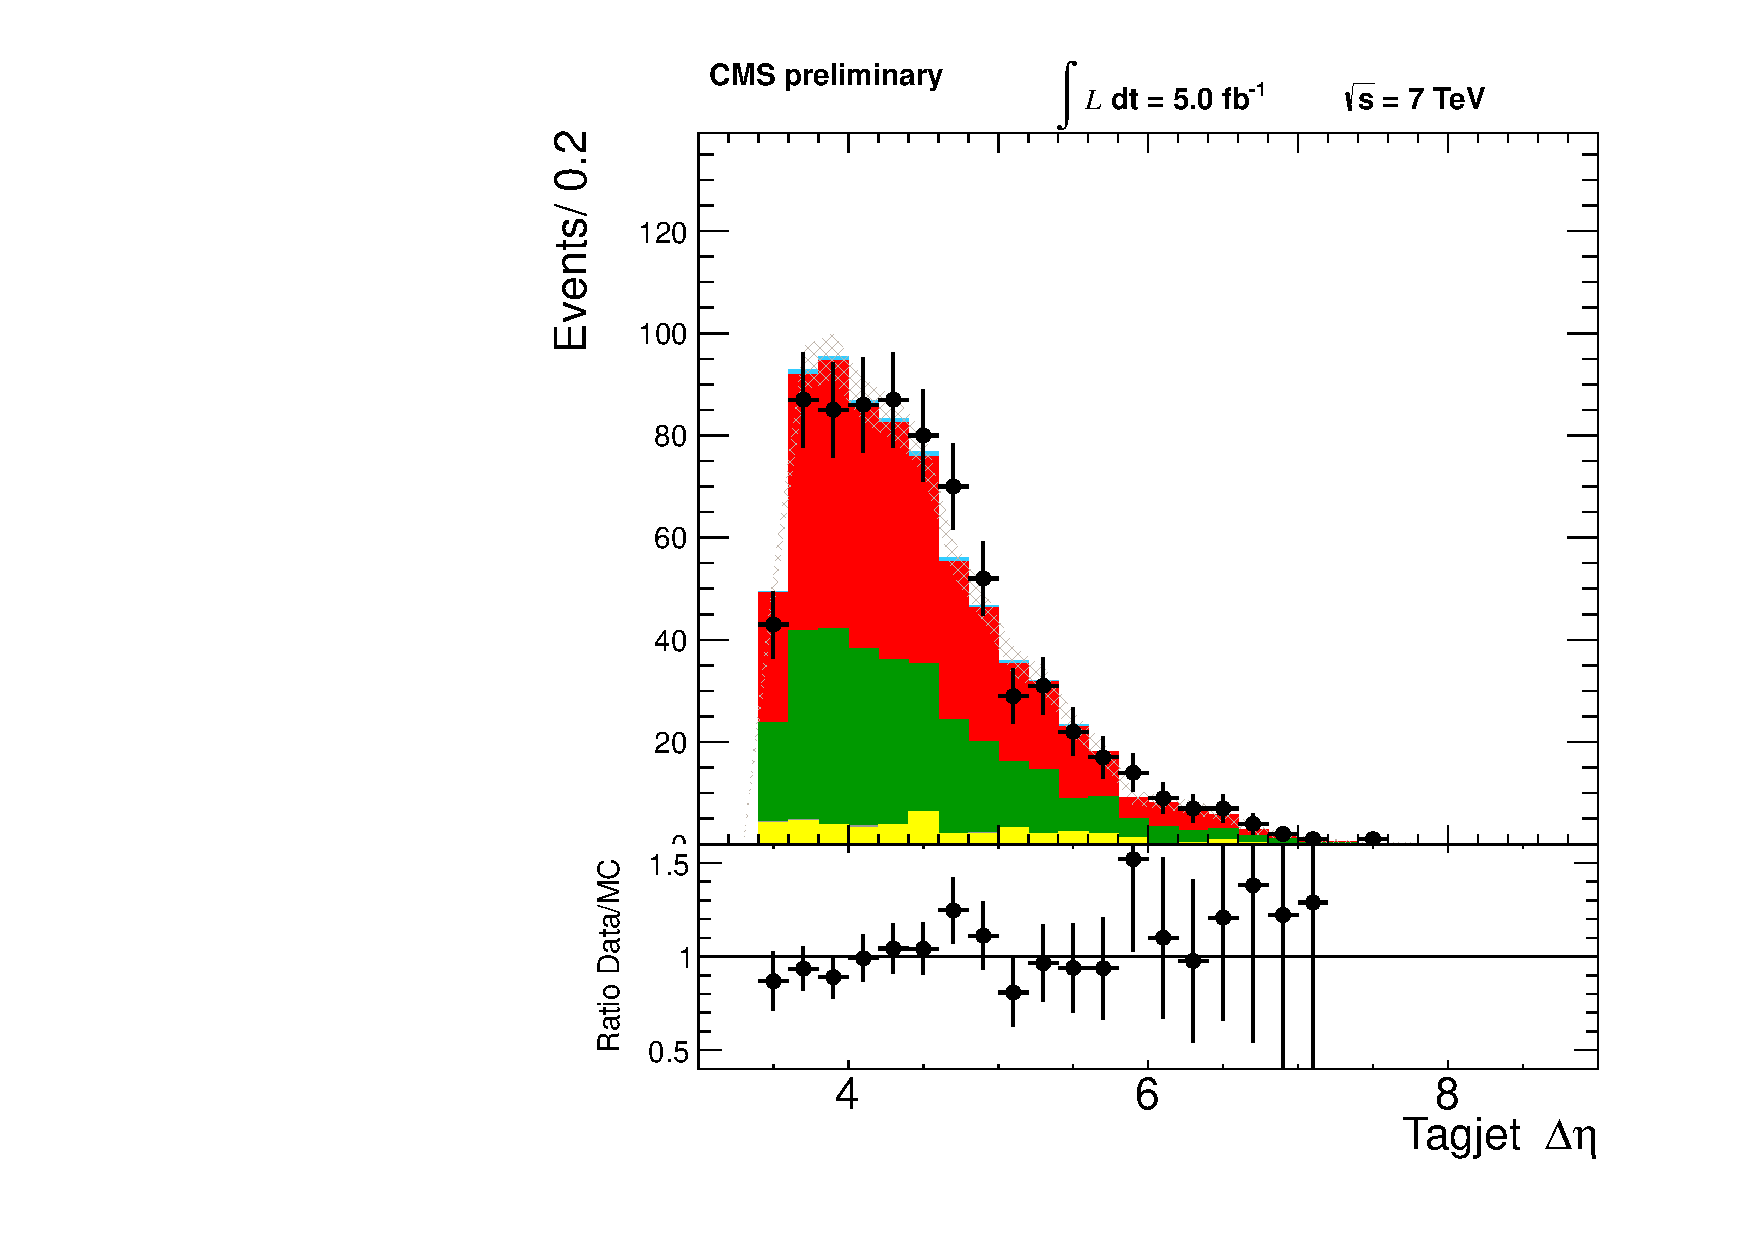
\includegraphics[width=0.49\textwidth]{figs/n-1_plots_mu/mu_vbftagjet_deta.pdf}
    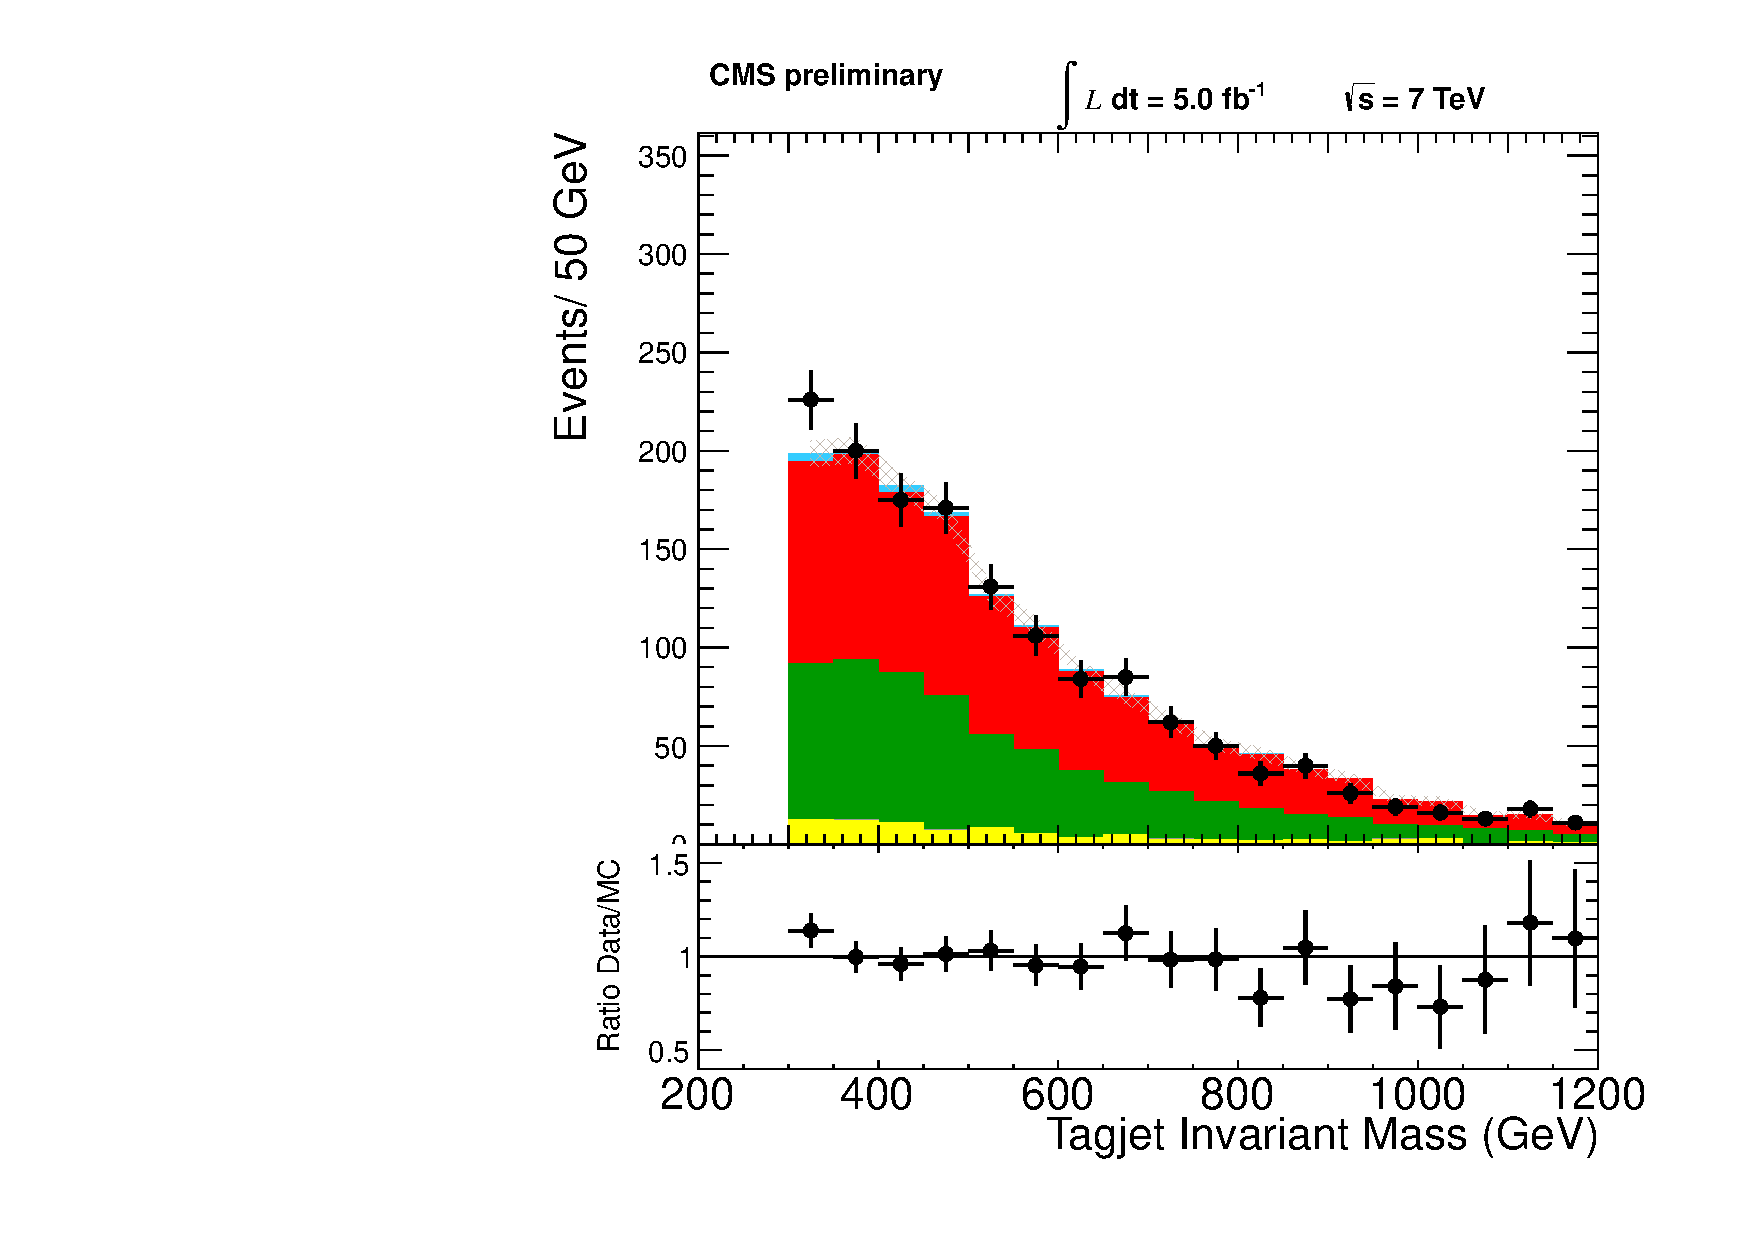
\includegraphics[width=0.49\textwidth]{figs/n-1_plots_mu/mu_vbftagjet_mass.pdf}
    \caption{Comparison of the VBF-tagged jet pair delta-eta (left)
      and invariant mass (right) distributions from data and MC for
      the muon+jets selection.  }
\label{fig:mu_tagjet_pair}}
\end{figure}

%%%%%%%%%%%%%%%%%%%%%%%%%%%%%%%%%
%%%%%%%%%%%%%%%%%%%%%%%

% angular variables
%%%%%%%%%%%%%%%%%%%%%%%%%%%%
%%%%%%%%%%%%%%%%%%%%%%%%%%%%
\begin{figure}[h!t]
  {\centering
    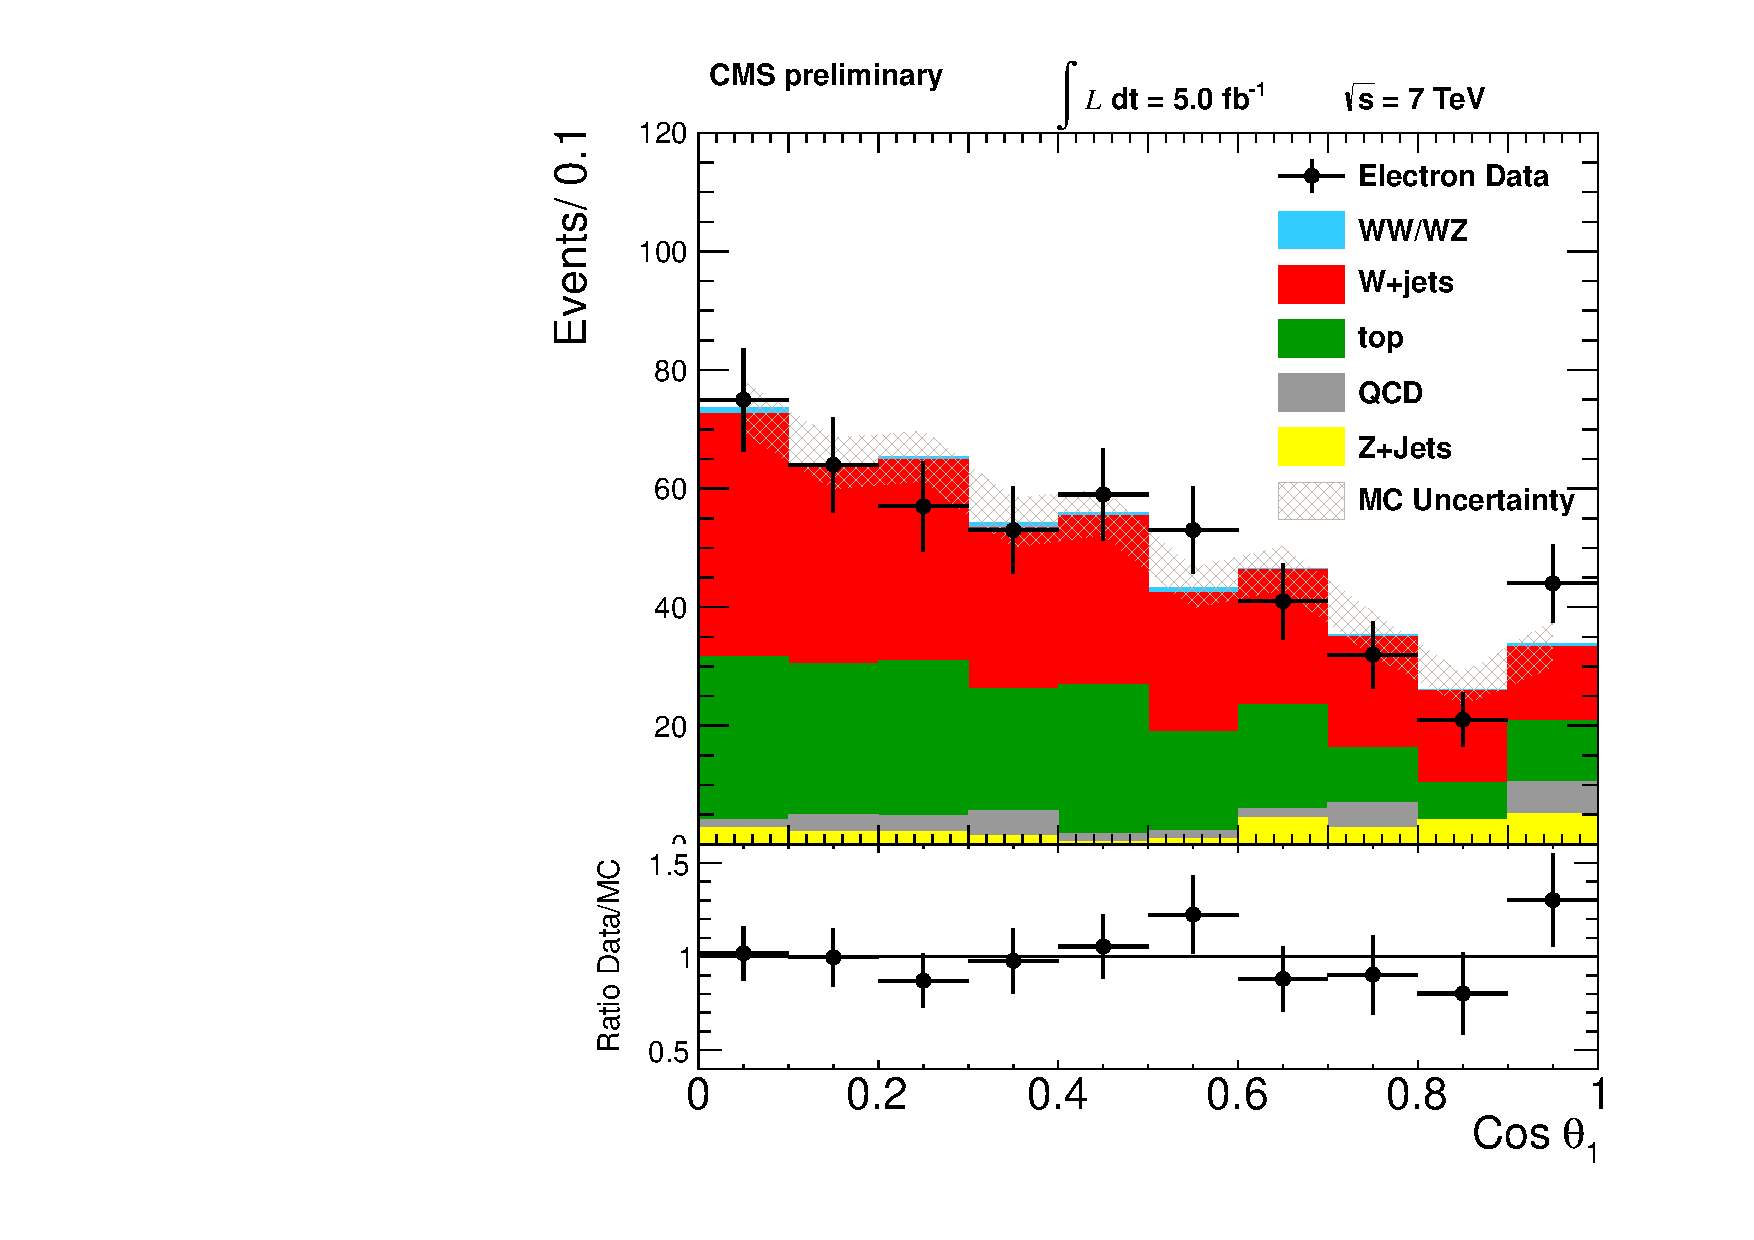
\includegraphics[width=0.49\textwidth]{figs/n-1_plots_el/el_vbfangha.pdf}
    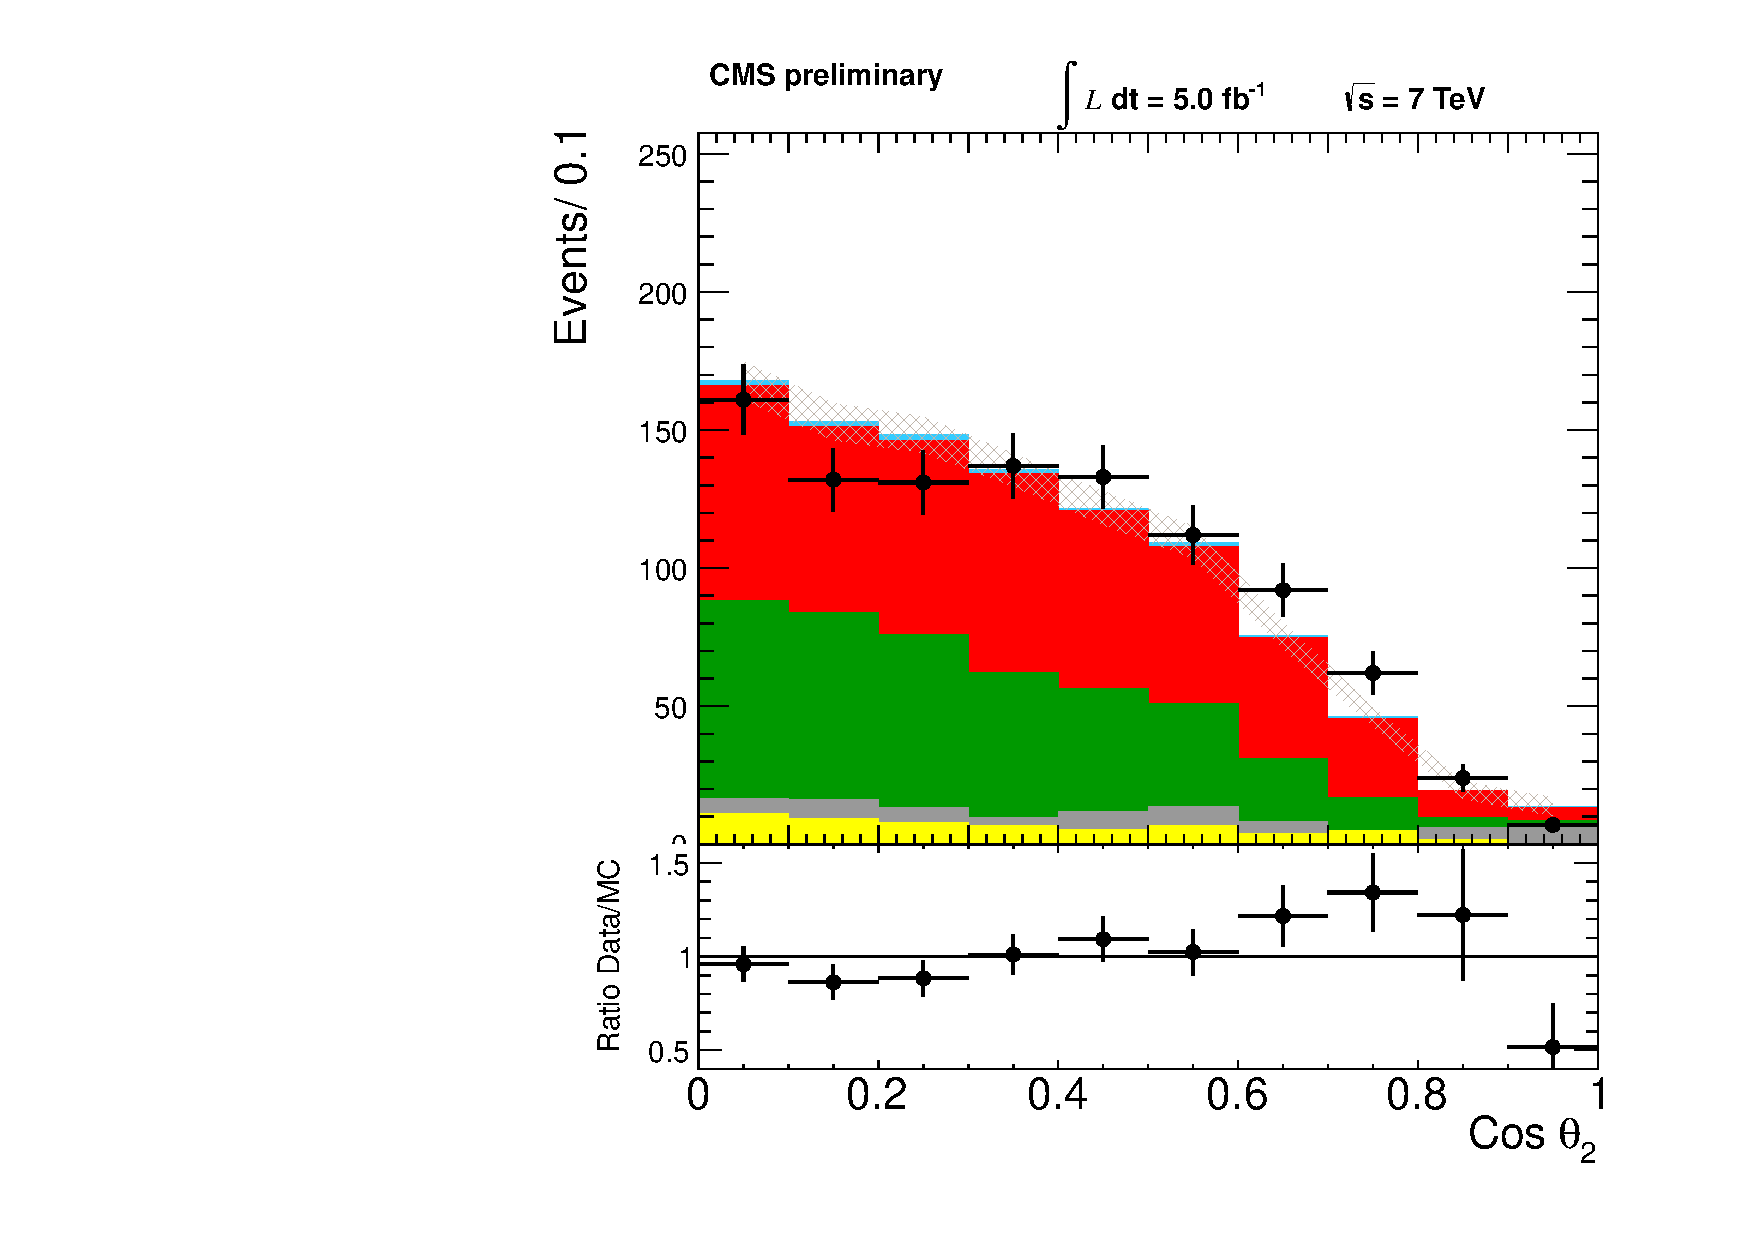
\includegraphics[width=0.49\textwidth]{figs/n-1_plots_el/el_vbfanghb.pdf}
    \caption{Comparison of the angular distributions for $\cos\theta_{1}$ (left)
   $\cos\theta_{2}$ (right) from data and MC for the electron+jets selection.}
\label{fig:el_theta}}
\end{figure}
%%%%%%%%%%%%%%%%%%%%%%%%%%%%
\begin{figure}[h!t]
  {\centering
     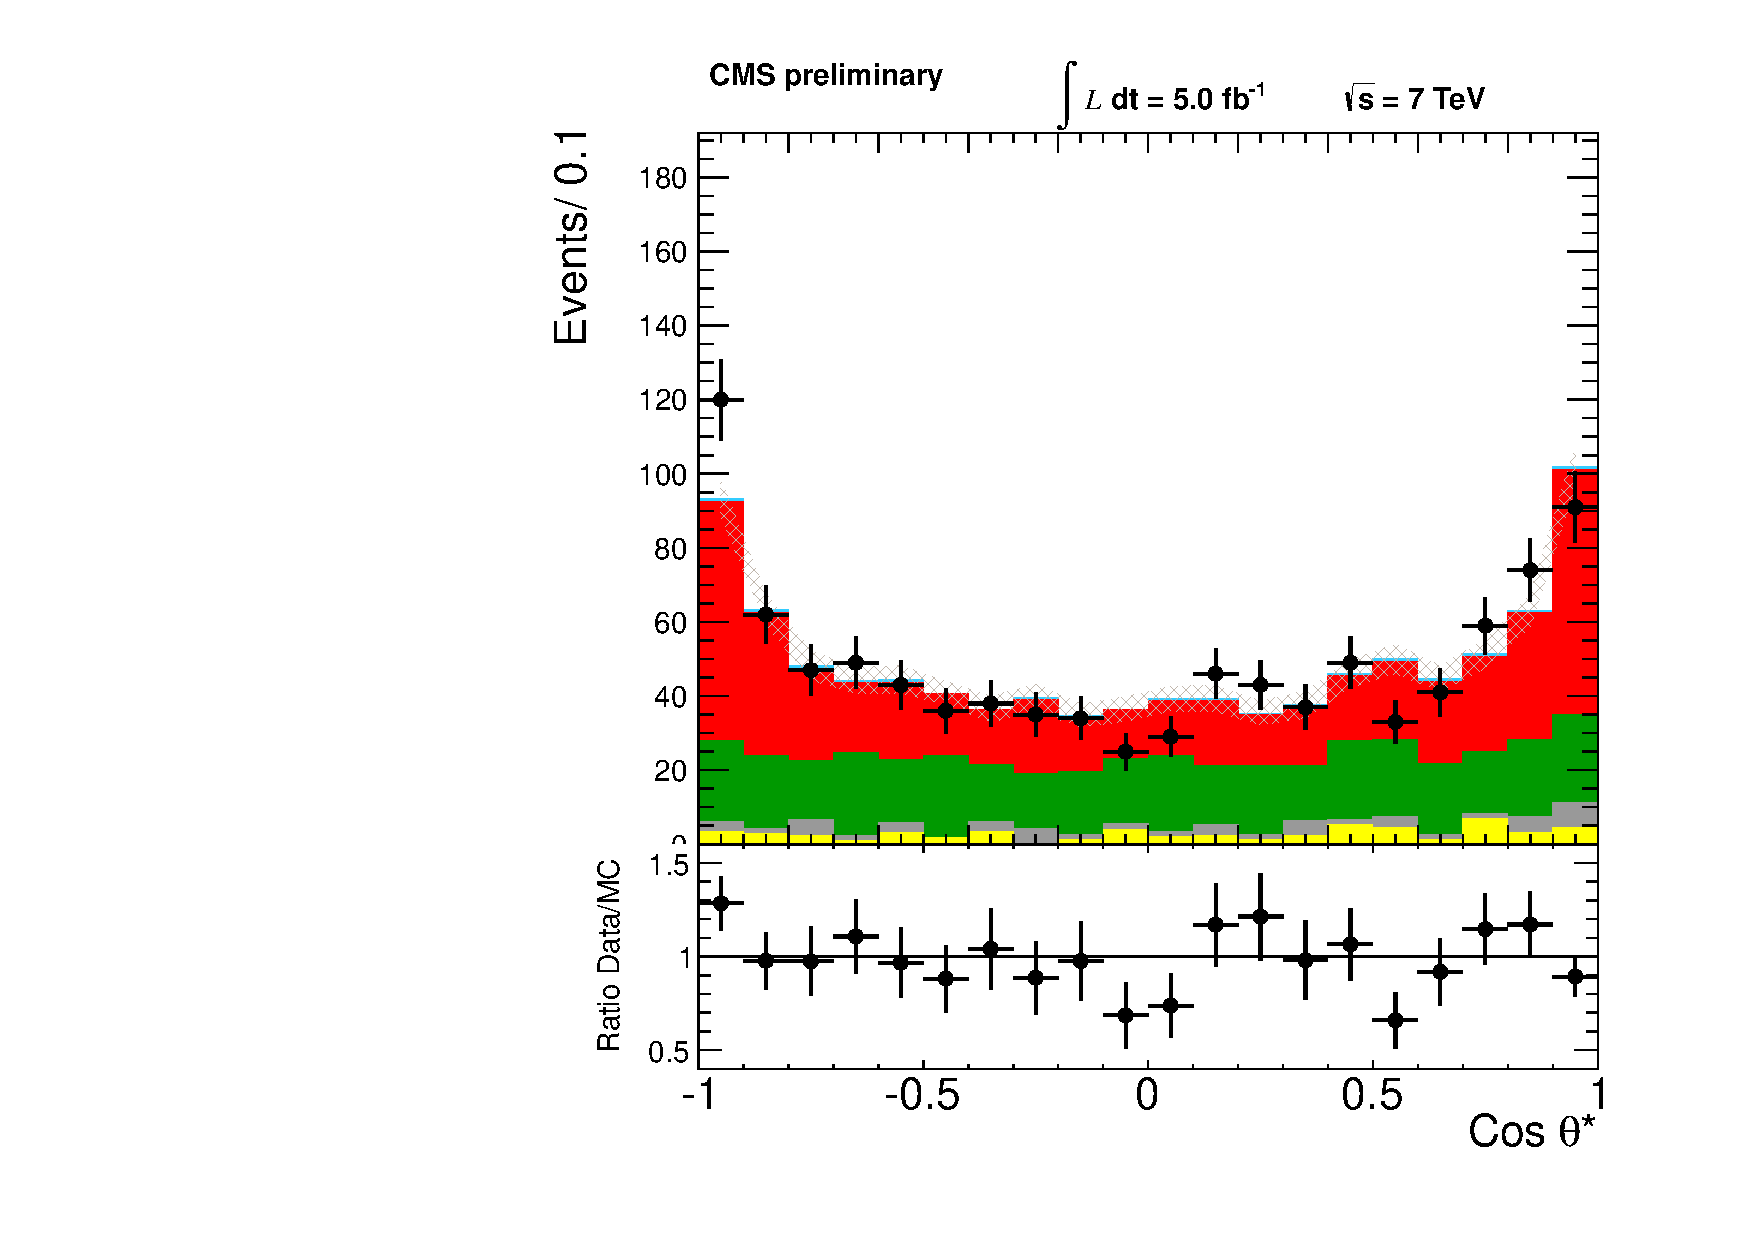
\includegraphics[width=0.49\textwidth]{figs/n-1_plots_el/el_vbfanghs.pdf}
    \caption{Comparison of the angular distributions for $\cos\theta^{\ast}$ from data and MC 
   for the electron+jets selection.}
\label{fig:el_thetas}}
\end{figure}
%%%%%%%%%%%%%%%%%%%%%%%%%%%%
\begin{figure}[h!t]
  {\centering
    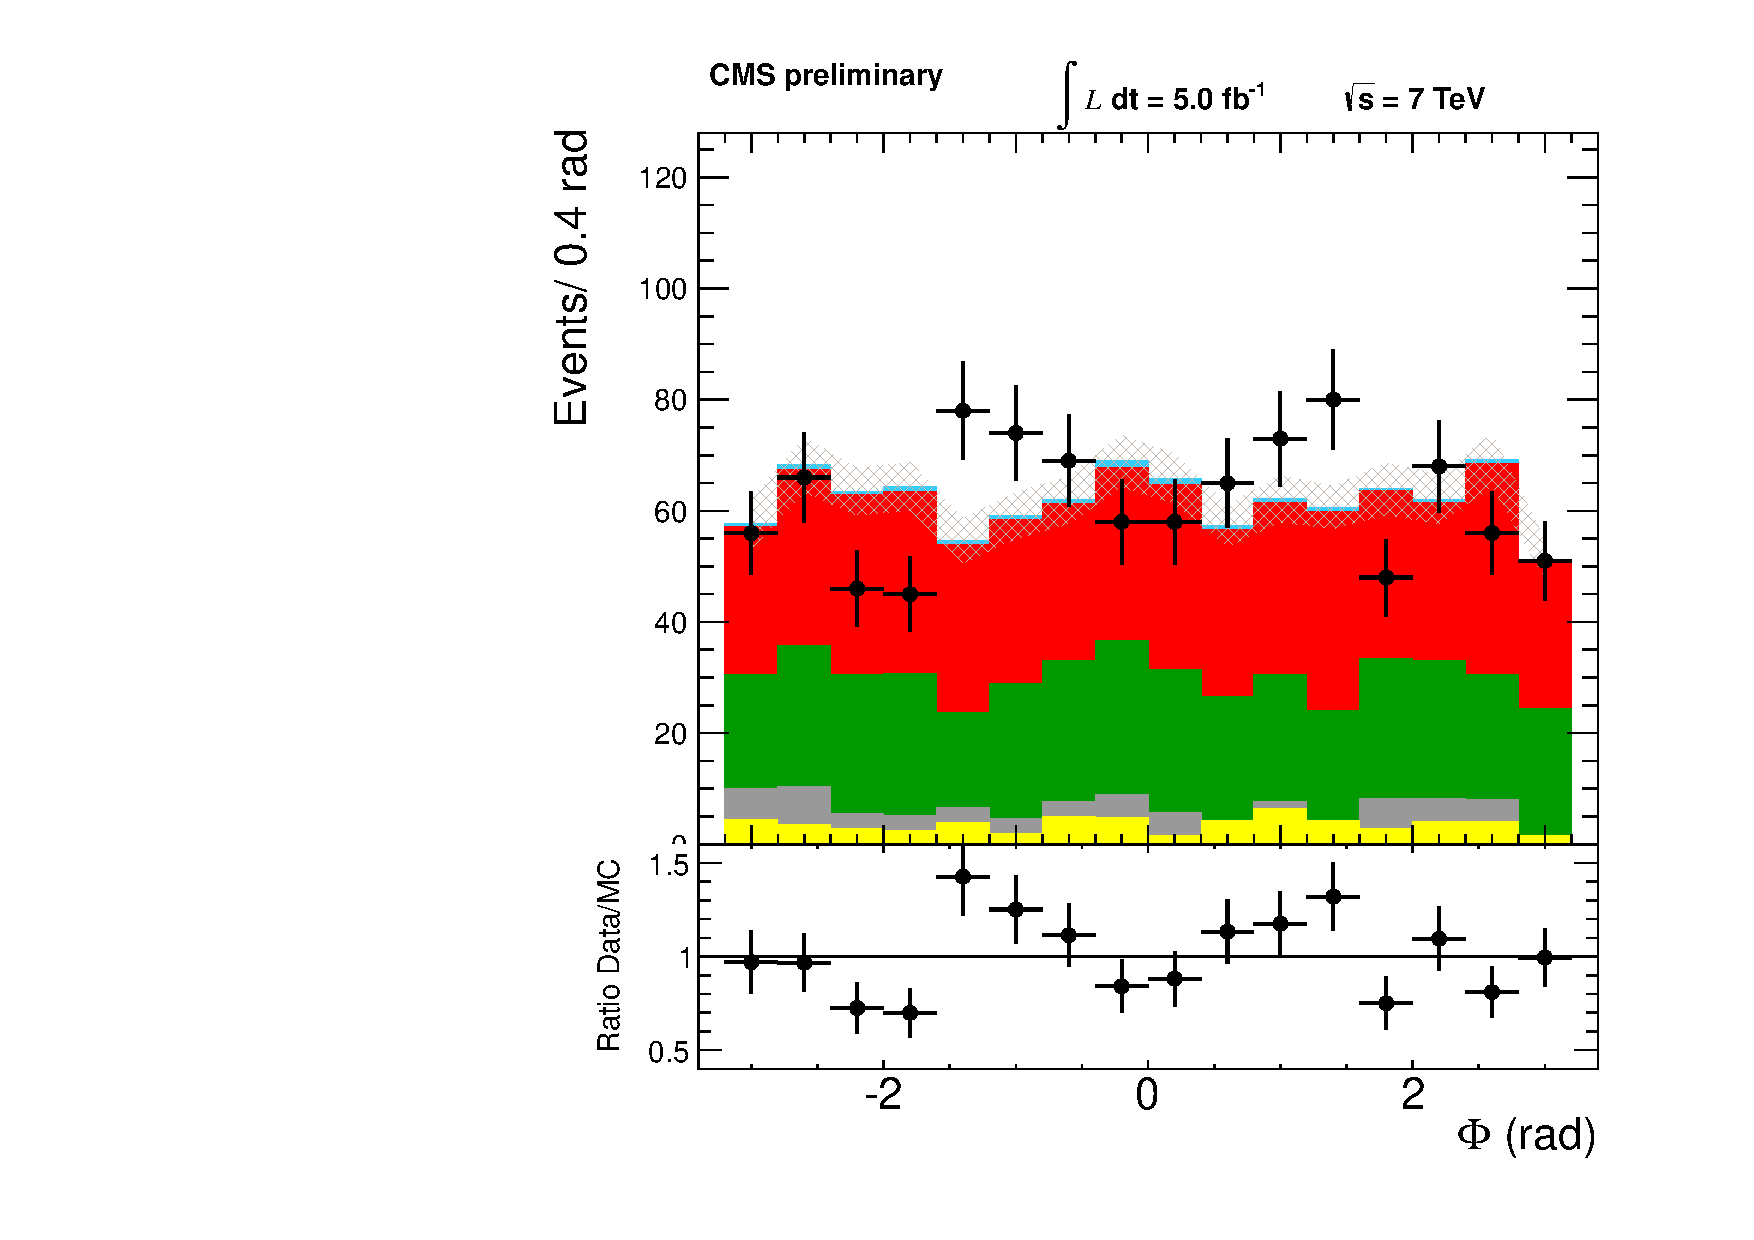
\includegraphics[width=0.49\textwidth]{figs/n-1_plots_el/el_vbfangphi.pdf}
    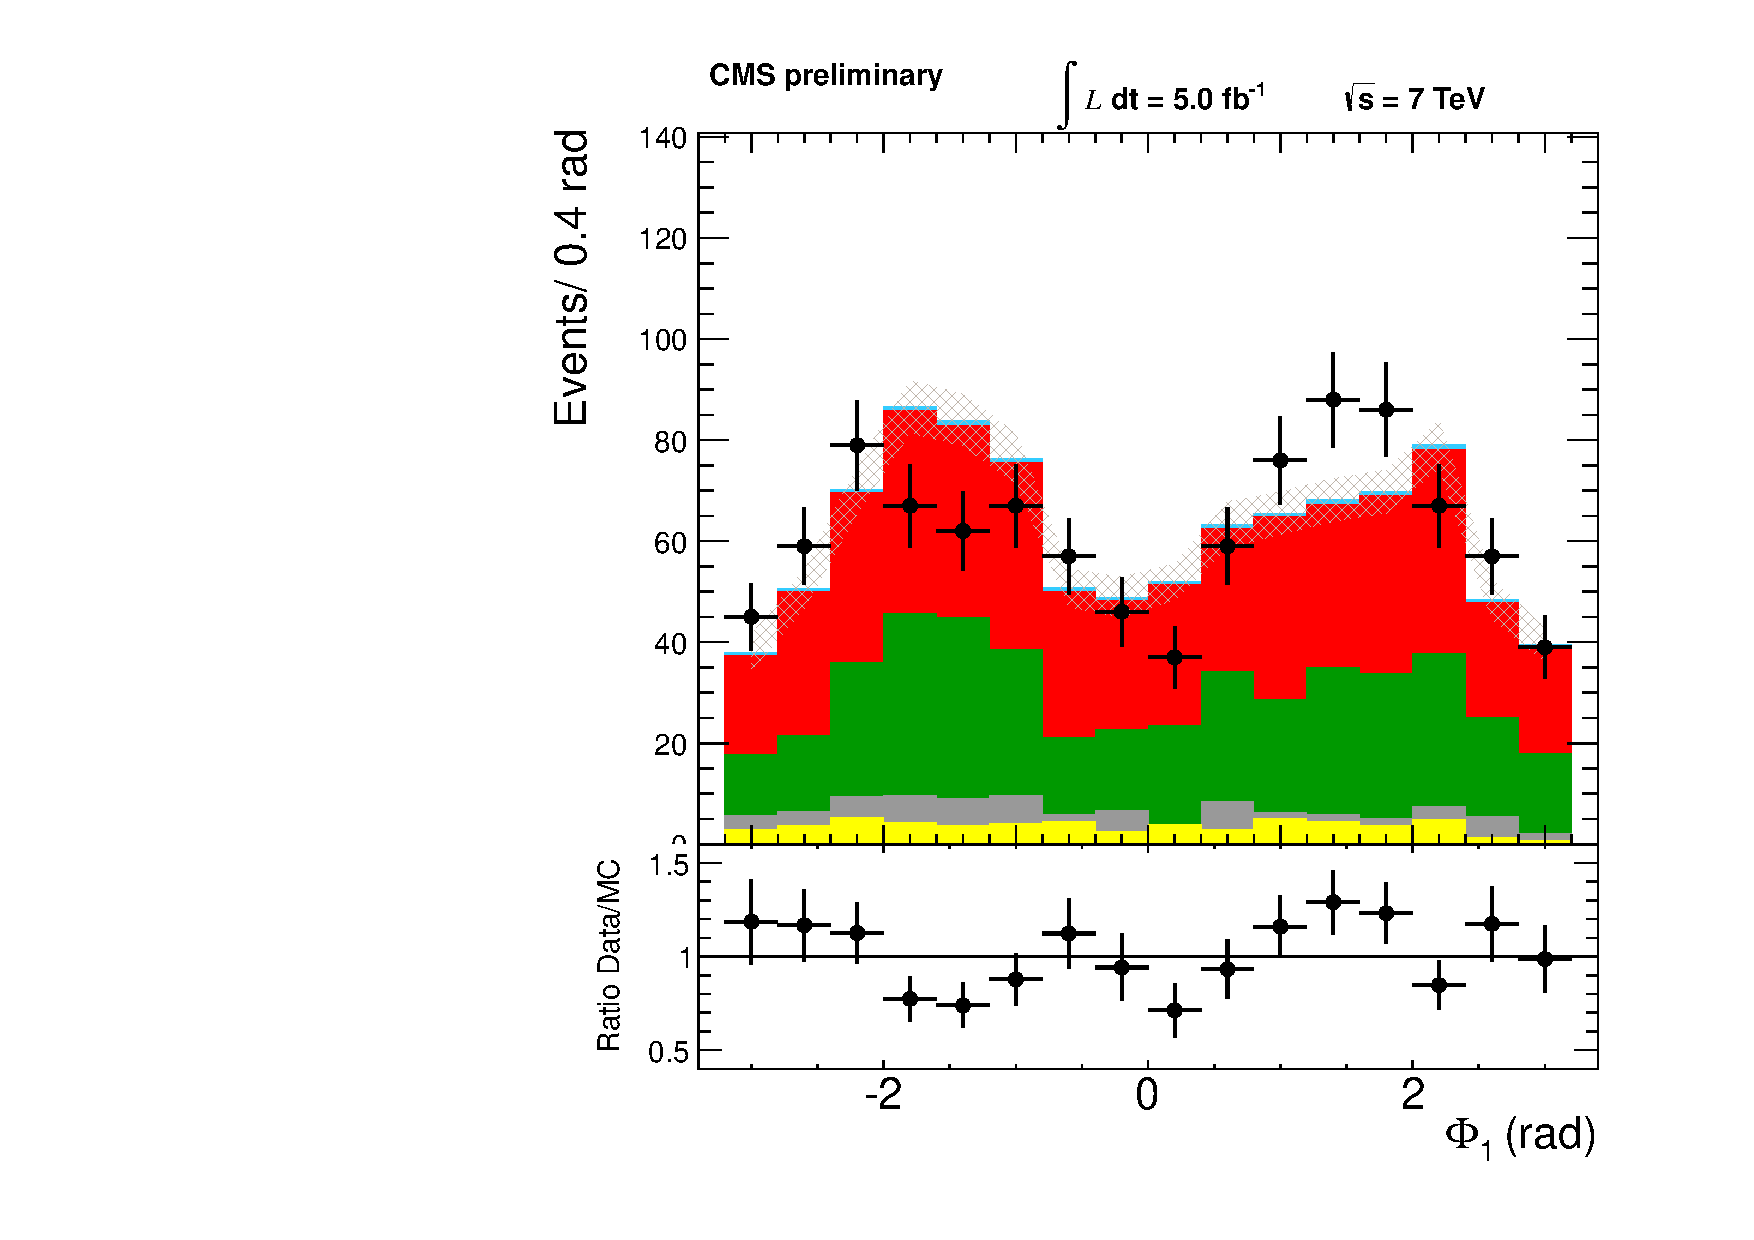
\includegraphics[width=0.49\textwidth]{figs/n-1_plots_el/el_vbfangphib.pdf}
    \caption{Comparison of the angular distributions for $\Phi$  (left)
    $\Phi_{1}$ (right) from data and MC for the 
    electron+jets selection.}
\label{fig:el_phi}}
\end{figure}

%%%%%%%%%%%%%%%%%%%%%%%%%%%%
\begin{figure}[h!t]
  {\centering
    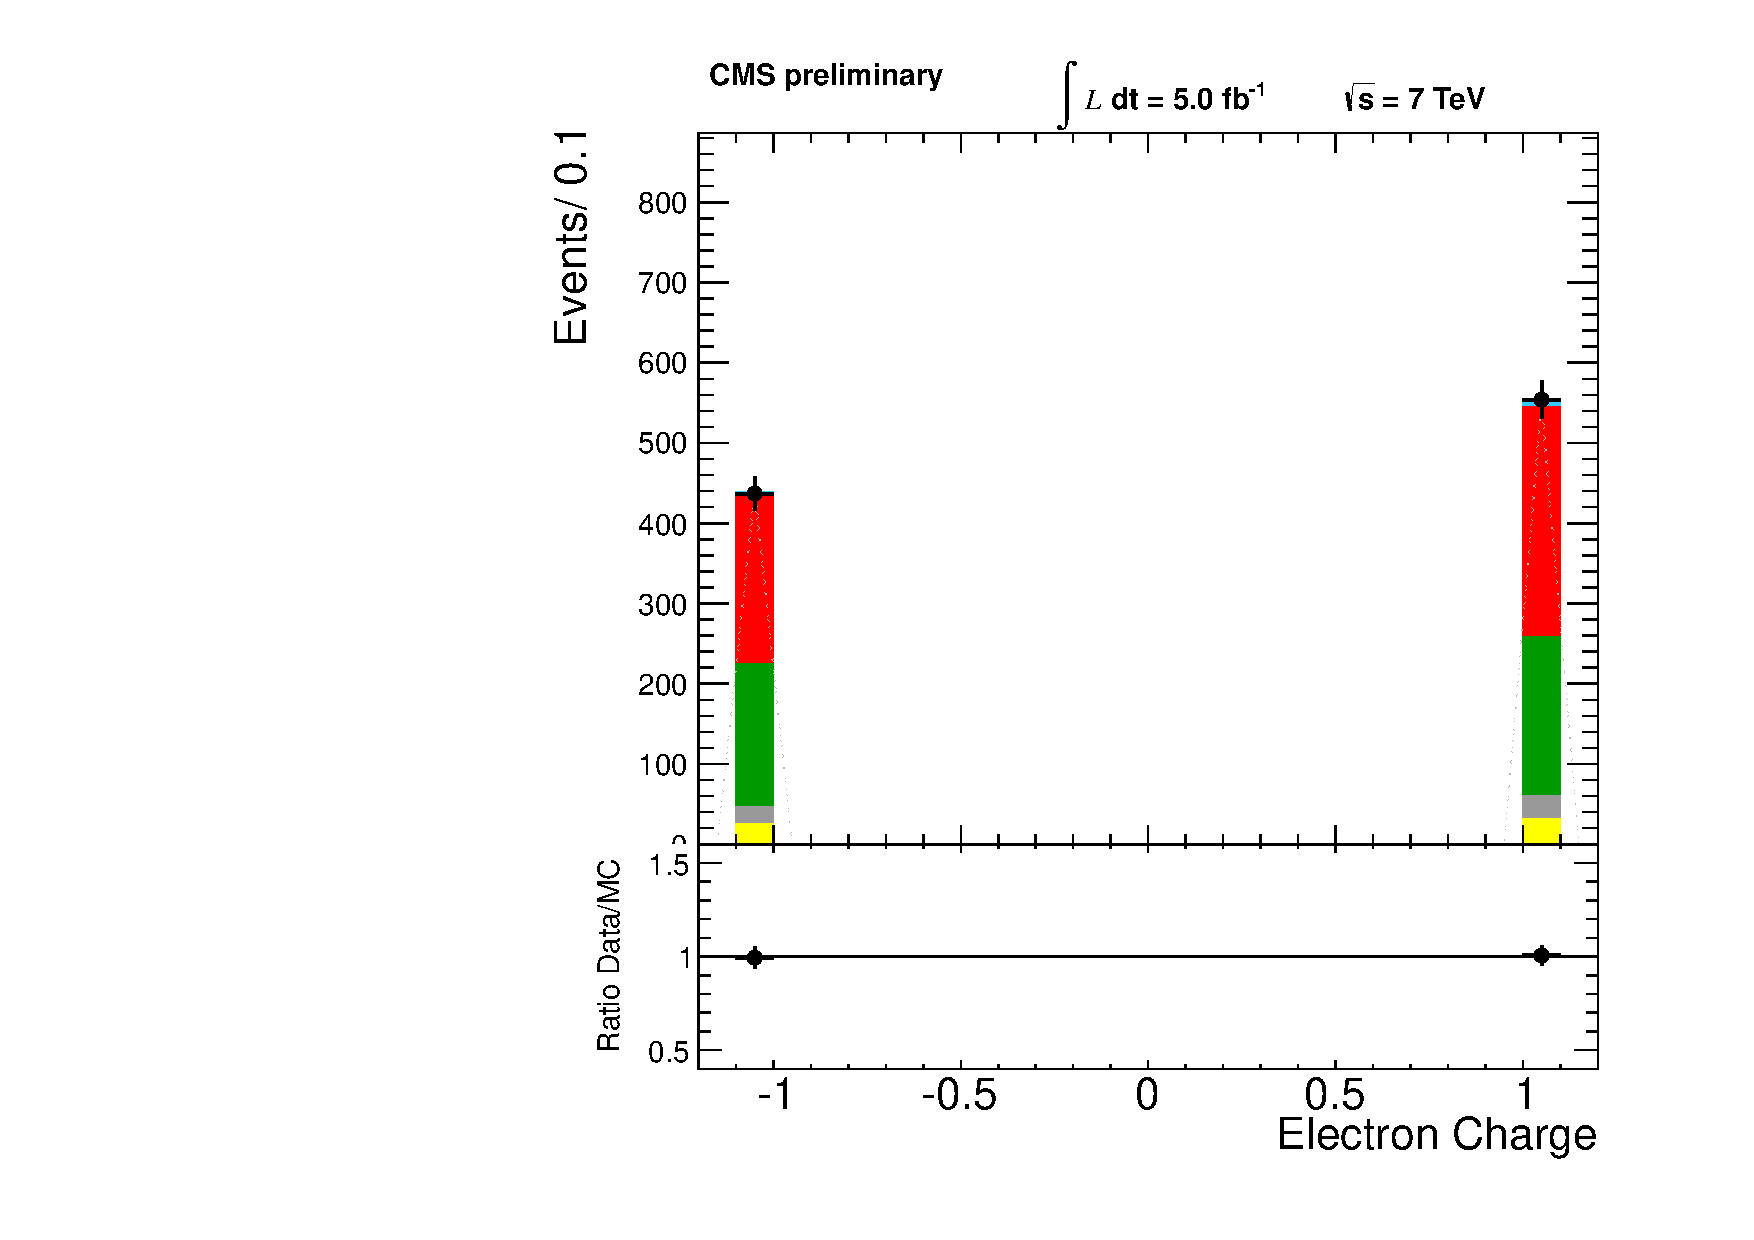
\includegraphics[width=0.49\textwidth]{figs/n-1_plots_el/el_vbfWelcharge.pdf}
    \caption{Comparison of the charge of the electron from data and MC for the electron+jets selection.}
\label{fig:el_chg}}
\end{figure}

\begin{figure}[h!t]
  {\centering
    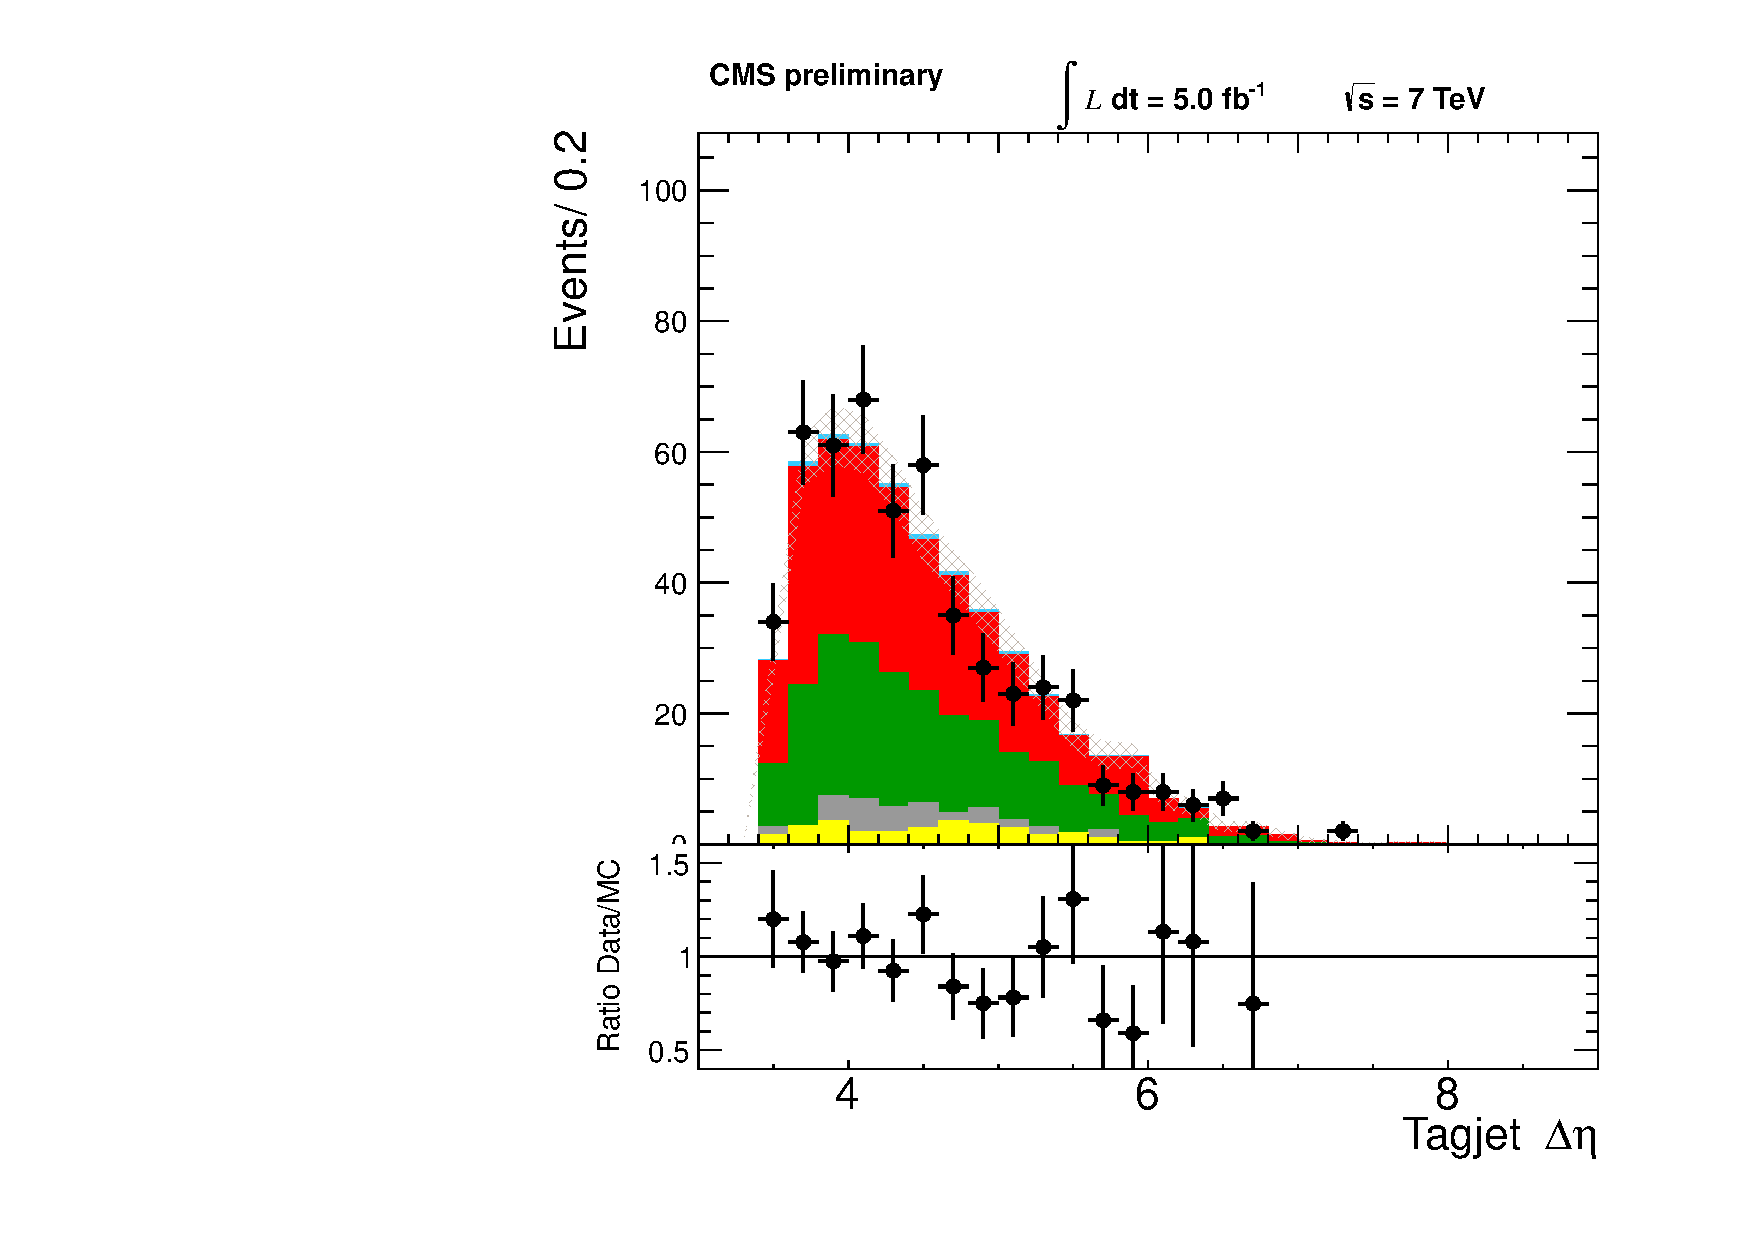
\includegraphics[width=0.49\textwidth]{figs/n-1_plots_el/el_vbftagjet_deta.pdf}
    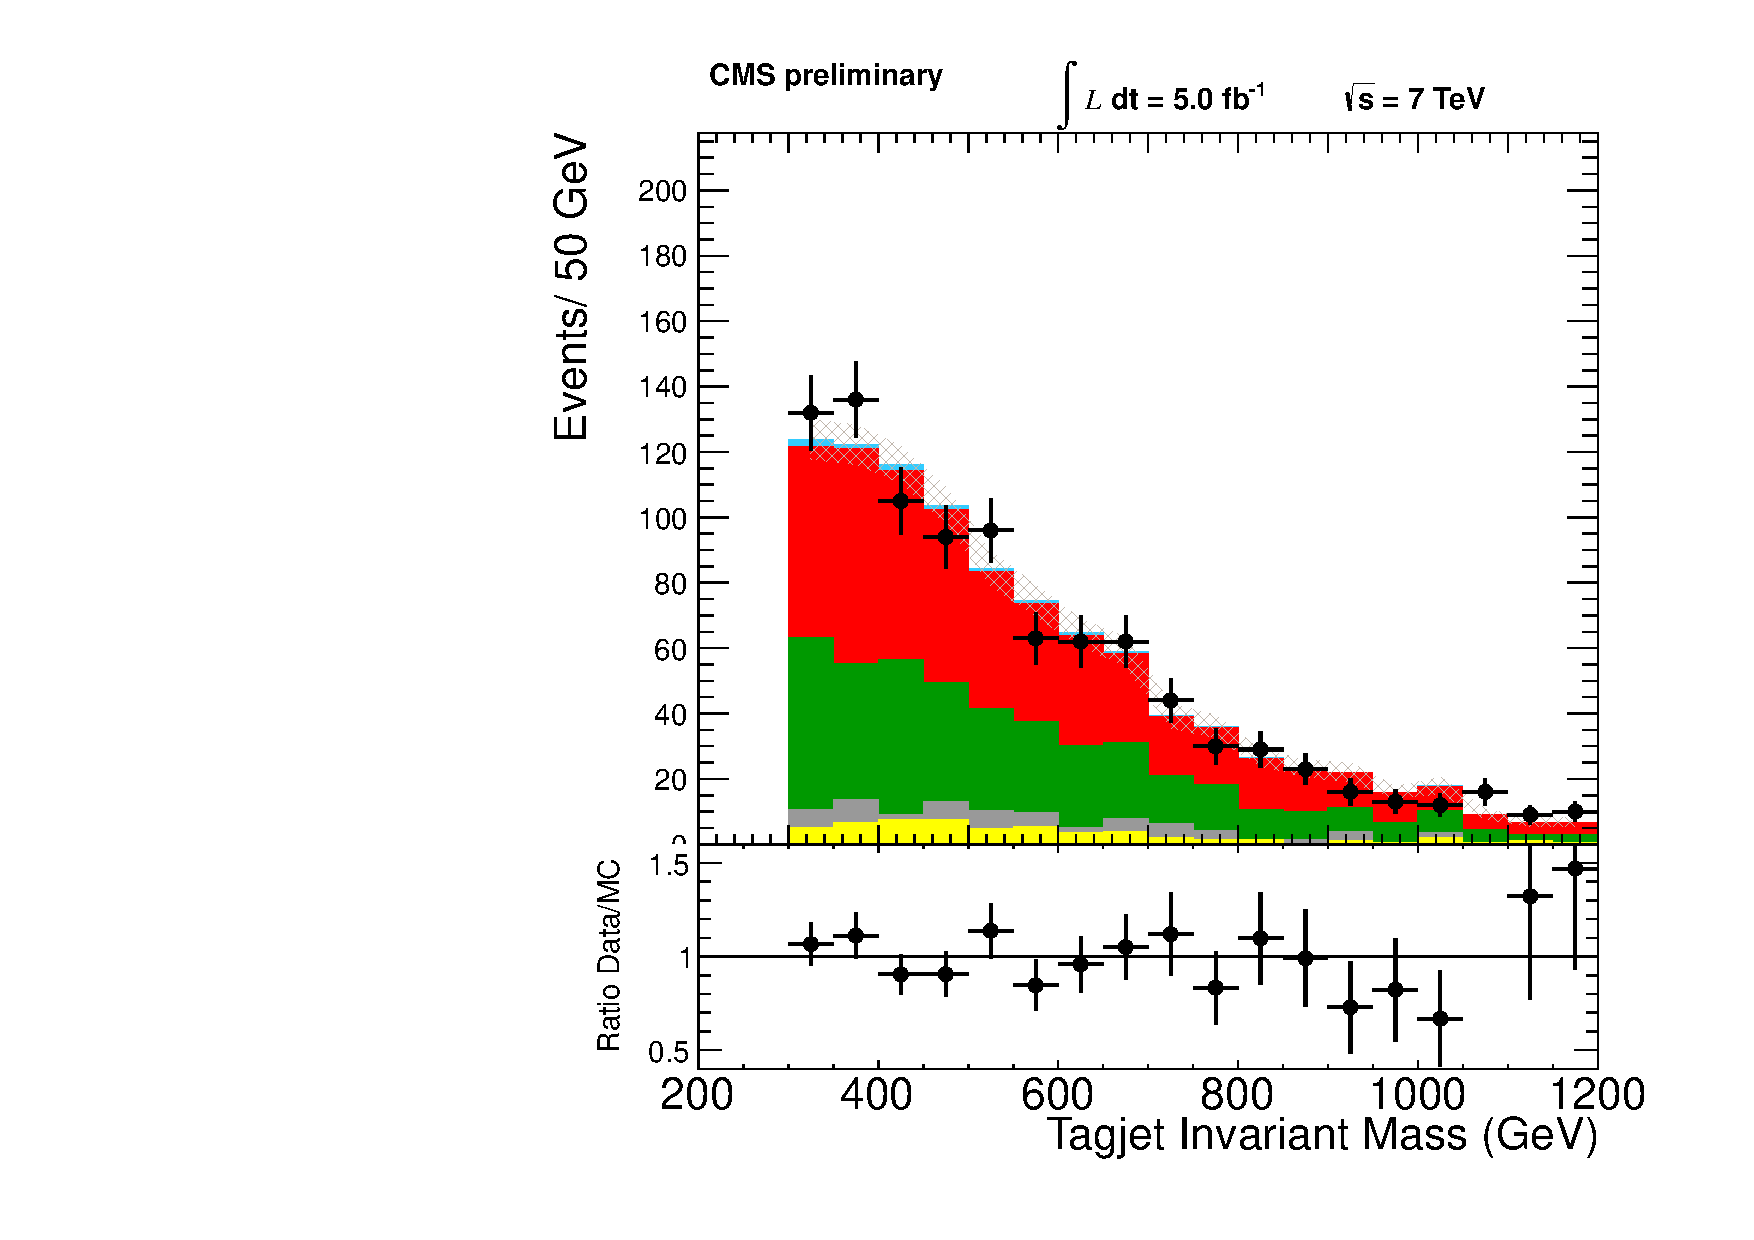
\includegraphics[width=0.49\textwidth]{figs/n-1_plots_el/el_vbftagjet_mass.pdf}
    \caption{Comparison of the VBF-tagged jet pair delta-eta (left)
      and invariant mass (right) distributions from data and MC for
      the electron+jets selection.  }
\label{fig:el_tagjet_pair}}
\end{figure}

% rapidity and pt of the WW system

%%%%%%%%%%%%%%%%%%%%%%%%%%%%
\begin{figure}[h!t]
  {\centering
    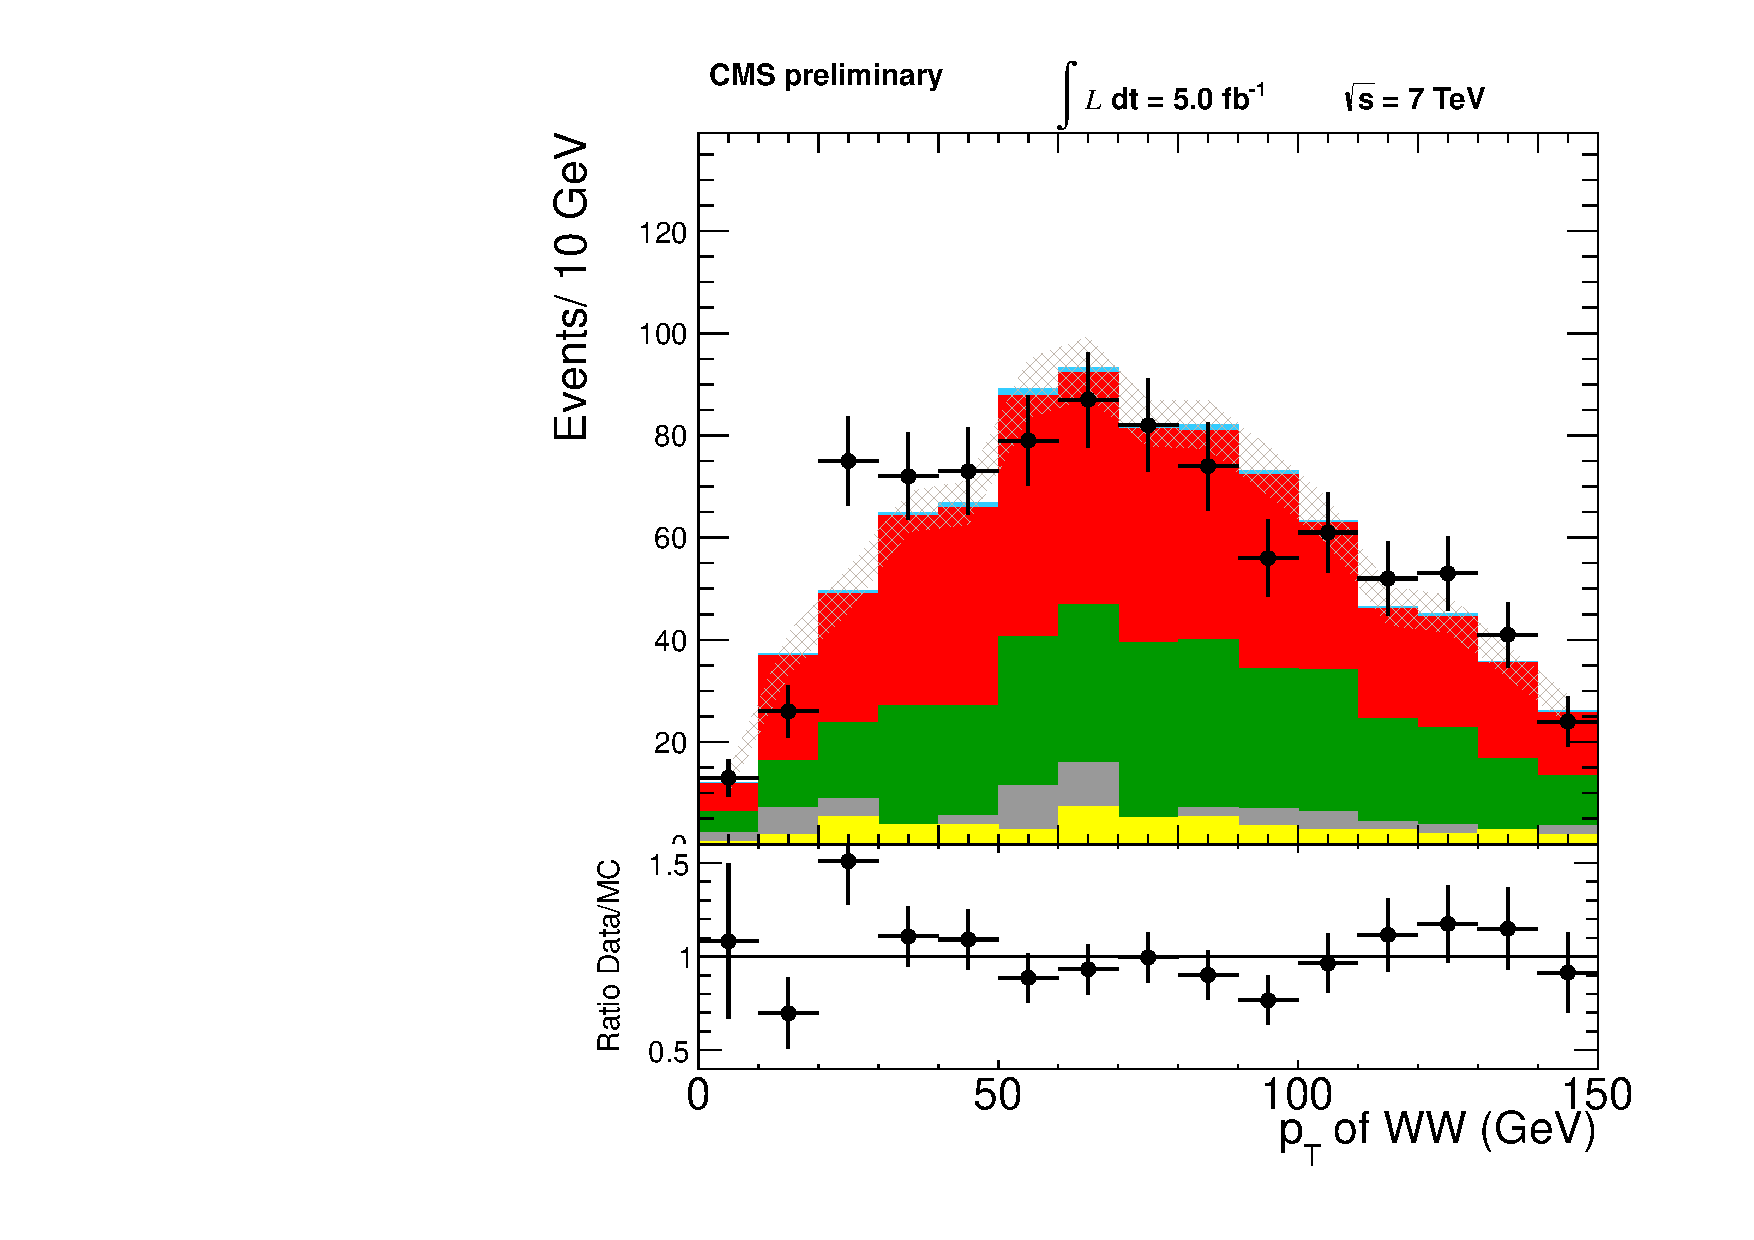
\includegraphics[width=0.49\textwidth]{figs/n-1_plots_el/el_vbfptlvjj.pdf}
    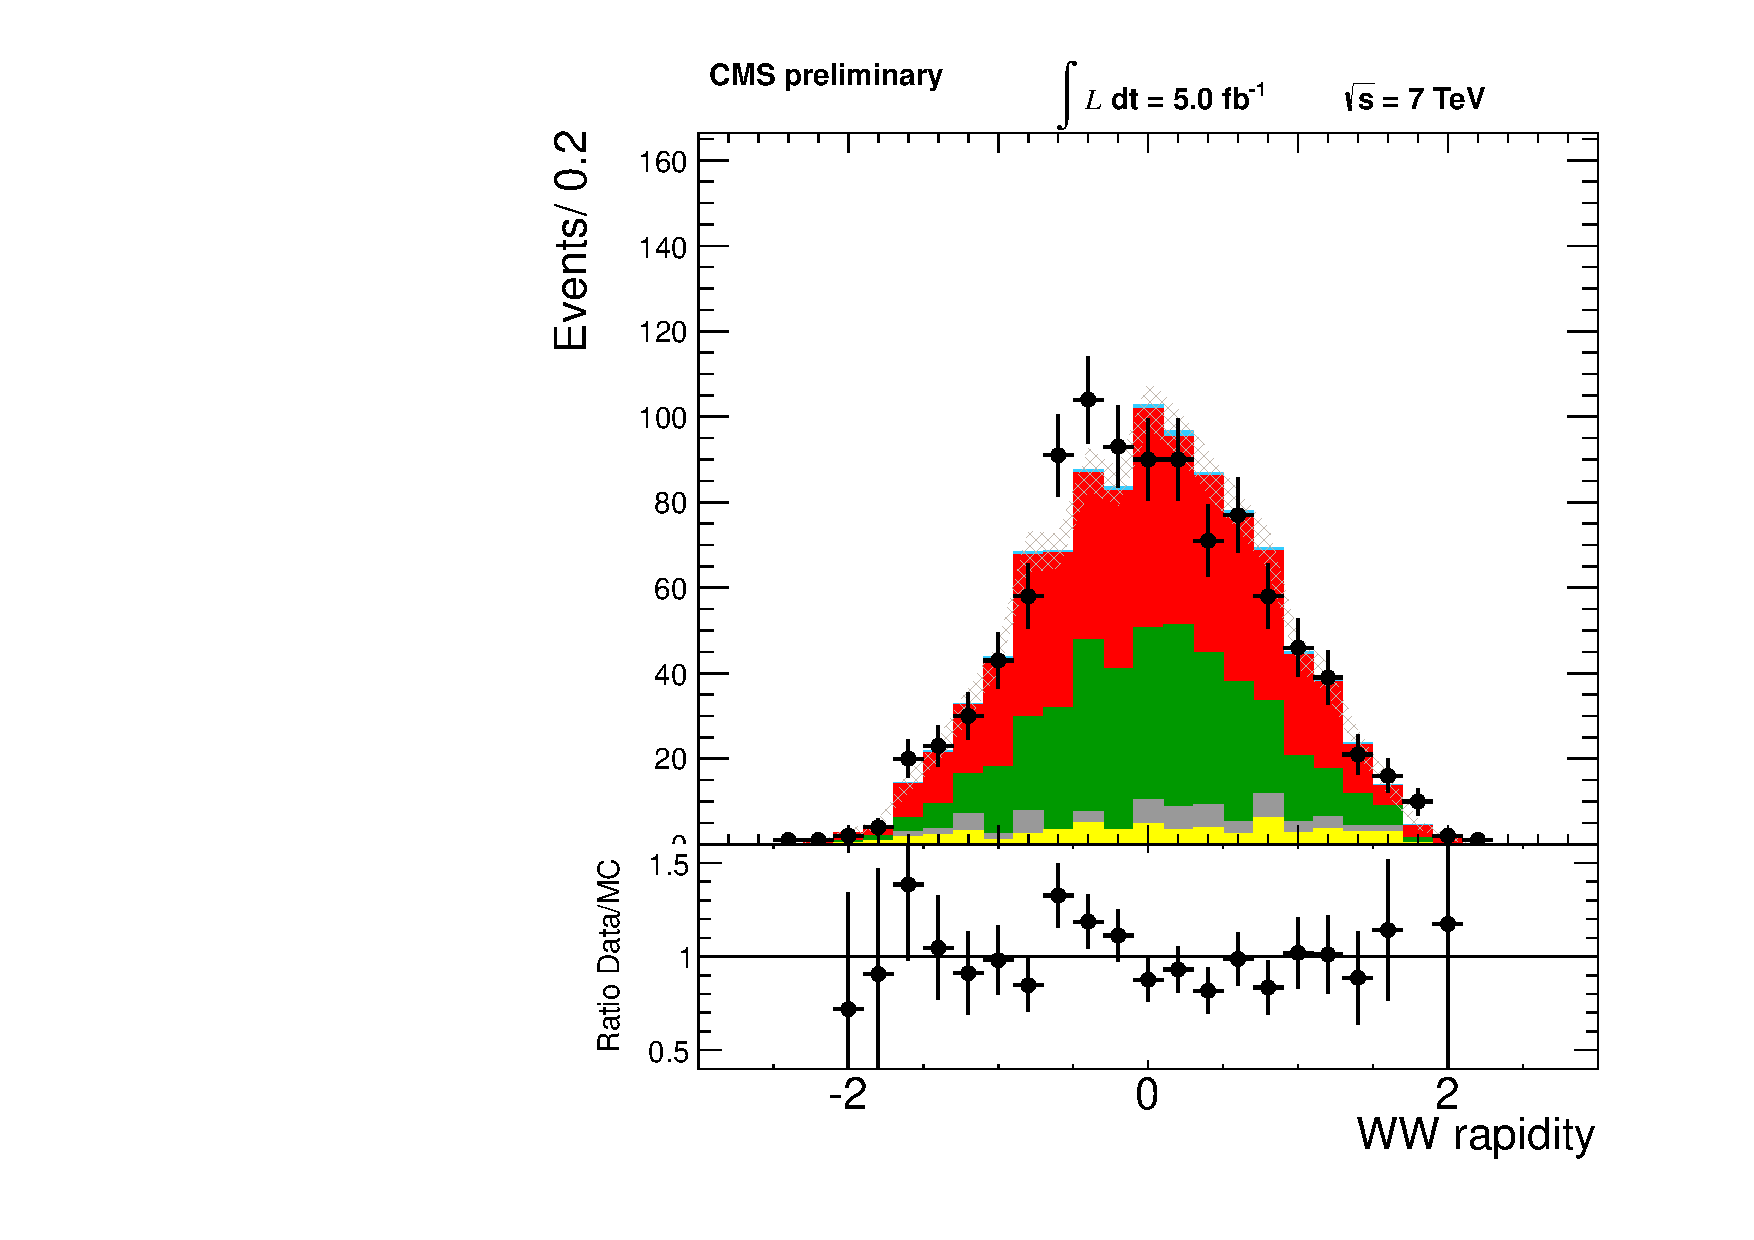
\includegraphics[width=0.49\textwidth]{figs/n-1_plots_el/el_vbfetalvjj.pdf}
    \caption{Comparison of the $p_{T}$ (left) $\eta$ (right) of the WW system
      from data and MC for the electron+jets selection.}
\label{fig:el_ww}}
\end{figure}

%%%%%%%%%%%%%%%%%%%%%%%%%%%%
\begin{figure}[h!t]
  {\centering
    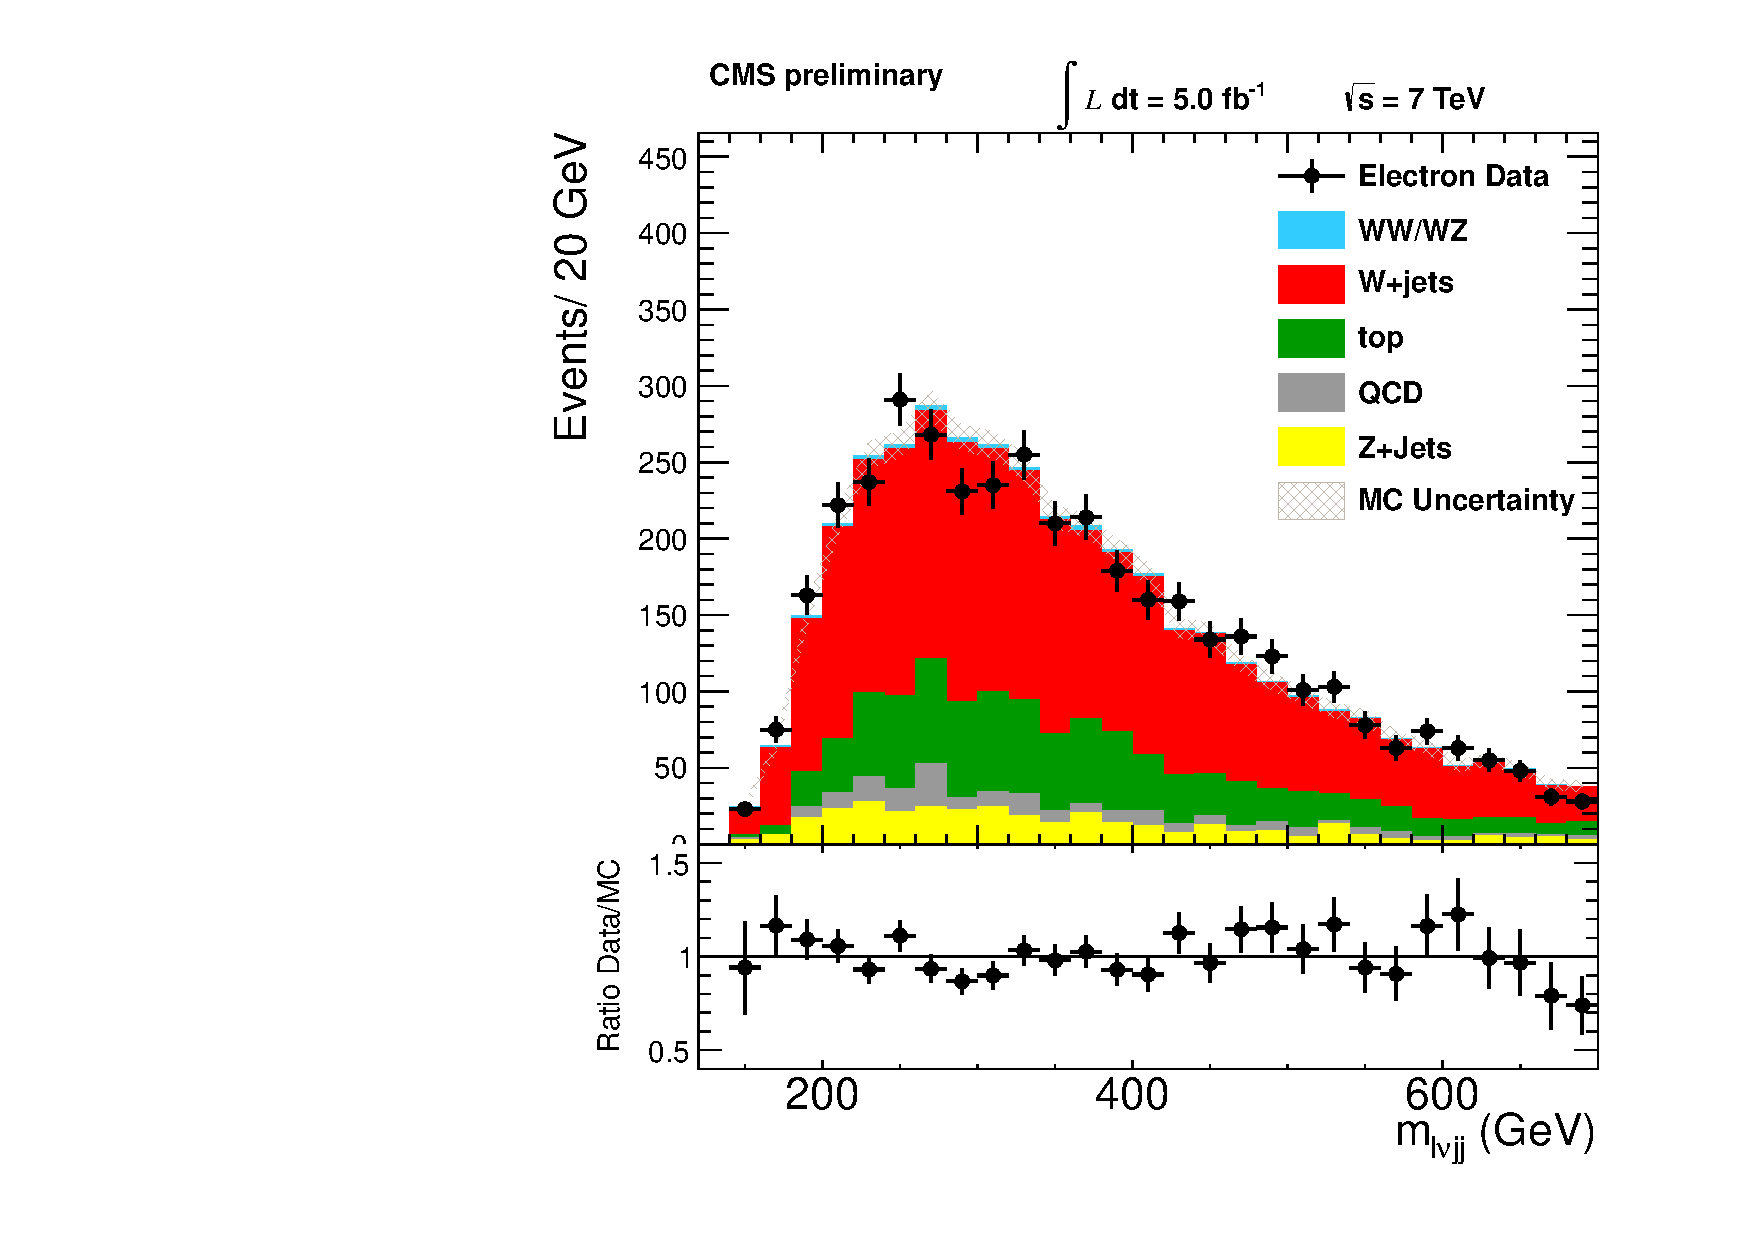
\includegraphics[width=0.49\textwidth]{figs/n-1_plots_el/el_vbfmlvjj.pdf}
    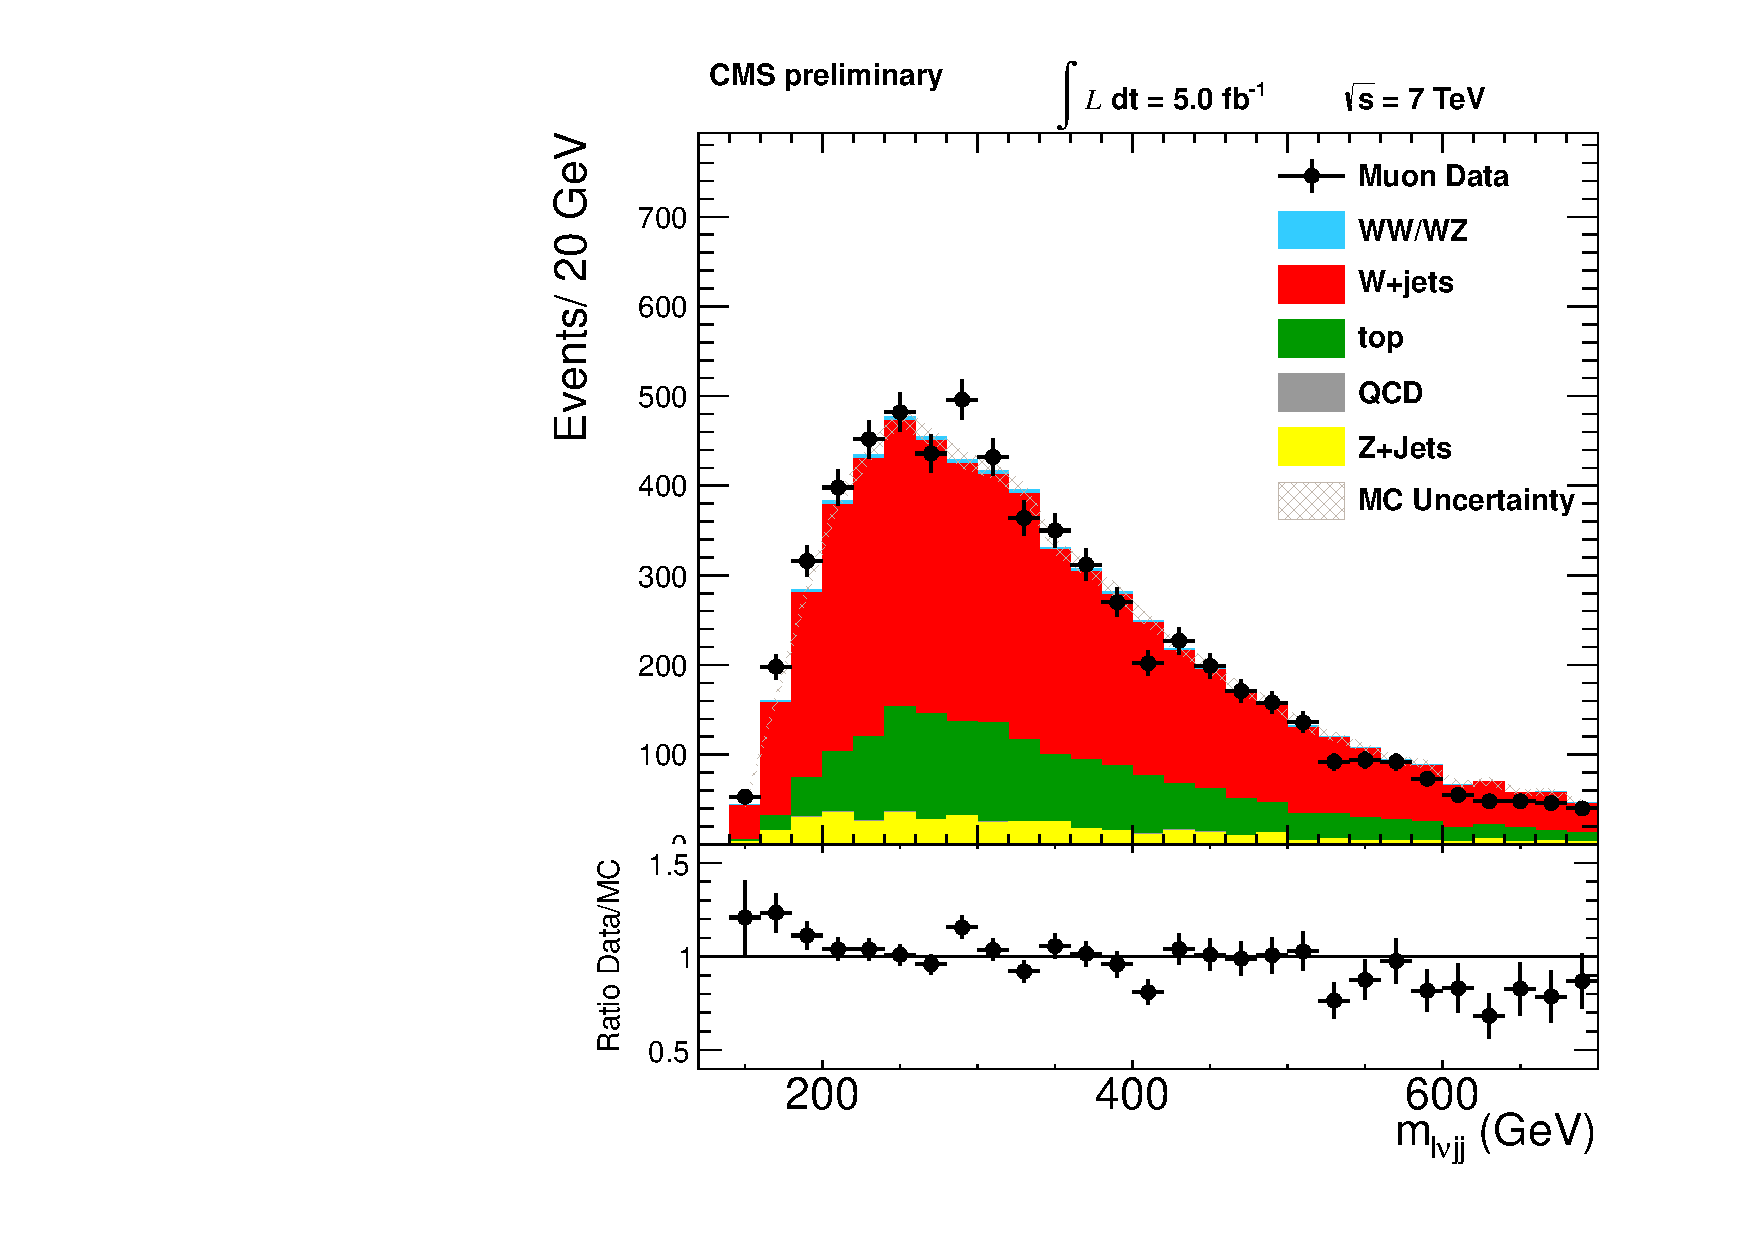
\includegraphics[width=0.49\textwidth]{figs/n-1_plots_mu/mu_vbfmlvjj.pdf}
    \caption{Comparison of the four-body invariant mass from data and MC for the electron+jets selection (left) 
             and muon+jets selection (right).}
\label{fig:lep_mlvjj}}
\end{figure}

%%%%%%%%%%%%%%%%%%%%%%%%%%%%%%%%%
%%%%%%%%%%%%%%%%%%%%%%%
\clearpage

\section{Optimization of likelihoods}
\label{sec:mvaoptimization}

Using a complete set of mostly uncorrelated variables we optimize each
Higgs mass points separately to distinguish between the Higgs signal
and the dominant backgrounds.  To achieve a better S/B separation we
split the data into two lepton flavors -- electron and muon, and
optimize each category separately. We implemented a multi-variate
analysis (MVA) and used likelihood as the only classifier. The details
of the likelihood optimization for gluon-gluon fusion are documented
in the CMS analysis note AN-2012/008; here we have implemented
the following modifications:

\begin{enumerate}
\item Two additional discriminating input variables were used to
optimize for VBF selection: the $|\Delta\eta|$ between tagged jets and
the invariant mass of the tagged jets.
\item The quark-gluon likelihood discriminant is not used.
\item Both W+4jets and $\ttbar$ background samples are used in the
training.
\end{enumerate}

We cut on the output of the classifier.  The value of the cut was
fixed at 0.2 for simplicity. The cut was made to be ``loose'' in
order to maintain sufficient statistics for the four-body shape fits
to converge.

\subsection{MVA input plots}

Figures~\ref{fig:inmva300}-\ref{fig:inmva500} display the input variable
distributions for signal and background for Higgs mass working points
300~GeV and 500~GeV.

%%%%%%%%%%%%%%%%%%%%%%%%%%%%
\begin{figure}[h!t]
  {\centering
    \includegraphics[width=0.90\textwidth]{figs/MVAplots/variables1_Mass300}
    \includegraphics[width=0.90\textwidth]{figs/MVAplots/variables2_Mass300}
    \caption{Inputs to the multivariate discriminant for SM Higgs mass of 300~GeV.}
\label{fig:inmva300}}
\end{figure}
\begin{figure}[h!t]
  {\centering
    \includegraphics[width=0.90\textwidth]{figs/MVAplots/variables1_Mass500}
    \includegraphics[width=0.90\textwidth]{figs/MVAplots/variables2_Mass500}
    \caption{Inputs to the multivariate discriminant for SM Higgs mass of 500~GeV.}
\label{fig:inmva500}}
\end{figure}

\clearpage

\subsection{Correlation among input variables}

Figures~\ref{fig:cormva300}-\ref{fig:cormva500} display the input
variable correlation matrices for signal and background processes for
Higgs mass working points 300~GeV and 500~GeV.

%%%%%%%%%%%%%%%%%%%%%%%%%%%%
\begin{figure}[h!t]
  {\centering
    \includegraphics[width=0.48\textwidth]{figs/MVAplots/CorrelationMatrixBackground_Mass300}
    \includegraphics[width=0.48\textwidth]{figs/MVAplots/CorrelationMatrixSignal_Mass300}
    \caption{Inputs to the multivariate discriminant for SM Higgs mass of 300~GeV.}
\label{fig:cormva300}}
\end{figure}
\begin{figure}[h!t]
  {\centering
    \includegraphics[width=0.48\textwidth]{figs/MVAplots/CorrelationMatrixBackground_Mass500}
    \includegraphics[width=0.48\textwidth]{figs/MVAplots/CorrelationMatrixSignal_Mass500}
    \caption{Inputs to the multivariate discriminant for SM Higgs mass of 500~GeV.}
\label{fig:cormva500}}
\end{figure}

\clearpage

\subsection{MVA likelihood output}

Figures~\ref{fig:outmva300}-\ref{fig:outmva500} display the input
variable correlation matrices for signal and background processes for
Higgs mass working points 300~GeV and 500~GeV.

\begin{figure}[h!t]
  {\centering
    \includegraphics[width=0.80\textwidth]{figs/MVAplots/Likelihood_output_Mass300}
    \caption{Outputs of the multivariate discriminant for SM Higgs mass of 300~GeV.}
\label{fig:outmva300}}
\end{figure}
\begin{figure}[h!t]
  {\centering
    \includegraphics[width=0.80\textwidth]{figs/MVAplots/Likelihood_output_Mass500}
    \caption{Outputs of the multivariate discriminant for SM Higgs mass of 500~GeV.}
\label{fig:outmva500}}
\end{figure}

\clearpage

%%%%%%%%%%%%%%%%%%%%%%%%%%%%%%%
%%%%%%%%%%%%%%%%%%%%%%%%%%%%%%%
%%%%%%%%%%%%%%%%%%%%%%%%%%%%%%%%%%%%%%%%%%%%%%%%%%%%%%%%%%%%%%%%%%%%
%%%%%%%%%%%%%%%%%%%%%%%%%%%%%%%%%%%%%%%%%%%%%%%%%%%%%%%%%%%%%%%%%%%%
%%%%%%%%%%%%%%%%%%%%%%%%%%%%%%%%%%%%%%%%%%%%%%%%%%%%%%%%%%%%%%%%%%%%
%%%%%%%%%%%%%%%%%%%%%%%%%%%%%%%%%%%%%%%%%%%%%%%%%%%%%%%%%%%%%%%%%%%%
%%%%%%%%%%%%%%%%%%%%%%%%%%%%%%%%%%%%%%%%%%%%%%%%%%%%%%%%%%%%%%%%%%%%
%%%%%%%%%%%%%%%%%%%%%%%%%%%%%%%%%%%%%%%%%%%%%%%%%%%%%%%%%%%%%%%%%%%%
%%%%%%%%%%%%%%%%%%%%%%%%%%%%%%%%%%%%%%%%%%%%%%%%%%%%%%%%%%%%%%%%%%%%
\section{Data driven QCD estimation}
\label{sec:qcd}
\label{sec:qcd_Uncertainty}

Ref.~\cite{CMS-AN-2011-110} describes a QCD background estimation
technique from 2011 data for the glu-glu fusion production
mechanism. It was determined that the percentage of QCD in data for
muons was 0.2$\pm$0.4\%, while the percentage of QCD in electron data
was approximately 6$\pm$3\% for two central jets. We adopt these fractions
here.  These are not optimized for the VBF final state and for a final
analysis the optimization needs to be done. However, they give the
correct order of magnitude for the QCD contribution to the background
for this analysis.

%%%%%%%
%%%%%%%%%%%%%%%%%%%%%%%%%%%%%%%%%%%%%%%%%%%%%%%%%%%%%%%%%%%%%%%%%%%%
%%%%%%%%%%%%%%%%%%%%%%%%%%%%%%%%%%%%%%%%%%%%%%%%%%%%%%%%%%%%%%%%%%%%
%%%%%%%%%%%%%%%%%%%%%%%%%%%%%%%%%%%%%%%%%%%%%%%%%%%%%%%%%%%%%%%%%%%%
%%%%%%%%%%%%%%%%%%%%%%%%%%%%%%%%%%%%%%%%%%%%%%%%%%
%%%%%%%%%%%%%%%%%%%%%%%%%%%%%%%%%%%%%%%%%%%%%%%%%%
\section{Modeling of W+jets background shape in \texorpdfstring{$m_{jj}$}{dijet invariant mass} }
\label{sec:wjetsShape}

The fit of the $m_{jj}$ spectrum is described in
\cite{CMS-AN-2011-110}, Section 10.  The line shapes used are detailed
as well as the parameters which float.  The projections of the fits to
data for each of the mass, flavor and jet number bins are in
Figs.~\ref{fig:mjj_mH300}--\ref{fig:mjj_mH600}.

%%%%%%%%%%%%%%%%%%%%%%%%%%%%%%%%%%%%%%%%%%%%%%%%%%
%%%%%%%%%%%%%%%%%%%%%%%%%%%%%%%%%%%%%%%%%%%%%%%%%%
%\clearpage
%%%%%%%%%%%%%%%%%%%%%%%%%%%%%%%%%%%%%%%%
%%%%%%%%%%%%%%%%%%%%%%%%%%%%%%%%%%%%%%%%
\section{Jet Energy Scale from the hadronic W in top quark events}
\label{sec:topw}
We take the results from \cite{CMS-AN-2011-110} in which it was
determined that any bias and uncertainty deriving from jet energy
scale is negligible.

%%%%%%%%%%%%%%%%%%%%%%%%%%%%%%%%%%%%%%%%
%%%%%%%%%%%%%%%%%%%%%%%%%%%%%%%%%%%%%%%%
\section{Kinematic fit}
\label{sec:kineFit}

Consistent with the analysis described in \cite{CMS-AN-2011-110}, we
perform a two constraint (2C) kinematic fit with one unknown, the
neutrino $z$ momentum component.  The constraints were that the
lepton-neutrino pair and the di-jet system both separately form an
invariant mass equal to the W mass to within its known width.  The
infrastructure of the fit uses standard CMS kinematic tools.  The four
particles are part of the fit, with a covariance matrix supplied in
the fit for the jets and the lepton.  The neutrino has small errors
assigned, by hand, to the unknown $z$ component of the momentum and
the $x$ and $y$ transverse components.  The starting value input to
the fit for the $x$ and $y$ components of the neutrino is the measured
missing transverse energy along the $x$ and $y$ axes, while the $z$
component is chosen as the solution with the smallest absolute value
(or the one that produces the neutrino closest to the lepton).  In
case no real solution is found, the real part of the solution is used.

%%%%%%%%%%%%%%%%%%%%%%%%%%%%%%%%%%%%%%%%%%%%%%%%%%
%%%%%%%%%%%%%%%%%%%%%%%%%%%%%%%%%%%%%%%%%%%%%%%%%%
%%%%%%%%%%%%%%%%%%%%%%%%%%%%%%%%%%%%%%%%%%%%%%%%%%
%%%%%%%%%%%%%%%%%%%%%%%%%%%%%%%%%%%%%%%%%%%%%%%%%%
\section{Extraction of W+jets background shape in
\texorpdfstring{$m_{WW}$}{diboson invariant mass} from data sidebands}
\label{sec:alphaExtraction}
The four-body mass shape of the W+jets background in the signal region
is estimated in a data driven way from sidebands in the $m_{jj}$
region.

As described in \cite{CMS-AN-2011-110}, we define three
regions in $m_{jj}$:
\begin{itemize}
\item lower sideband region (SBL):  $m_{jj} \in$ [55,65]~GeV
\item signal region: $m_{jj} \in $ [65,95]~GeV
\item upper sideband region (SBH): $m_{jj} \in$ [95,115] for $M_H<$250~GeV, [95,200]~GeV  for $M_H\ge$250~GeV, 
\end{itemize}

However, whereas in \cite{CMS-AN-2011-110} the optimal combination of
SBL and SBH is determined for each working point, for this
analysis the $m_{\ell\nu jj}$ shapes within the signal region for all
14 working points is determined entirely by the upper sideband region,
SBH (``$\alpha = 0$'').

The distributions of the $m_{\ell\nu jj}$ shape in data are shown in
Figs.~\ref{fig:mlnujj_WpJShape_mH300}--\ref{fig:mlnujj_WpJShape_mH600}
for various Higgs mass points and lepton flavors.  Because these
shapes in general do not have copious statistics in them we fit the
shape using a binned likelihood method to an exponential shape.  This
exponential shape is used as the template for the W+jets background of
the $m_{\ell\nu jj}$.  The uncertainty in the decay constant for the
exponential shape utilized as a systematic uncertainty in the limit
setting.
%%%%%%%%%%%%%%%%%%%%
%%%%%%%%%%%%%%%%%%%%
%%%%%%%%%%%%%%%%%%%%
\begin{figure}[h!t]
  {\centering
\subfigure[]{
    \includegraphics[width=0.48\textwidth]{figs/fitplots/H300_Mlvjj_Muon_2jets_WpJShape}
}
\subfigure[]{
    \includegraphics[width=0.48\textwidth]{figs/fitplots/H300_Mlvjj_Electron_2jets_WpJShape}
}
\caption{$M_H = 300$~GeV point. The distribution of the $m_{\ell\nu
jj}$ shape in data and its smooth parametrization.  The two plots
correspond to muon and electron event categories, respectively. }
\label{fig:mlnujj_WpJShape_mH300}
}
\end{figure}
%%%%%%%%%%%%%%%%%%%%
%%%%%%%%%%%%%%%%%%%%
%%%%%%%%%%%%%%%%%%%%
\begin{figure}[h!t]
  {\centering
\subfigure[]{
    \includegraphics[width=0.48\textwidth]{figs/fitplots/H350_Mlvjj_Muon_2jets_WpJShape}
}
\subfigure[]{
    \includegraphics[width=0.48\textwidth]{figs/fitplots/H350_Mlvjj_Electron_2jets_WpJShape}
}
\caption{$M_H = 350$~GeV point. The distribution of the $m_{\ell\nu
jj}$ shape in data and its smooth parametrization.  The two plots
correspond to muon and electron event categories, respectively. }
\label{fig:mlnujj_WpJShape_mH350}
}
\end{figure}
%%%%%%%%%%%%%%%%%%%%
%%%%%%%%%%%%%%%%%%%%
%%%%%%%%%%%%%%%%%%%%
\begin{figure}[h!t]
  {\centering
\subfigure[]{
    \includegraphics[width=0.48\textwidth]{figs/fitplots/H400_Mlvjj_Muon_2jets_WpJShape}
}
\subfigure[]{
    \includegraphics[width=0.48\textwidth]{figs/fitplots/H400_Mlvjj_Electron_2jets_WpJShape}
}
\caption{$M_H = 400$~GeV point. The distribution of the $m_{\ell\nu
jj}$ shape in data and its smooth parametrization.  The two plots
correspond to muon and electron event categories, respectively. }
\label{fig:mlnujj_WpJShape_mH400}
}
\end{figure}
%%%%%%%%%%%%%%%%%%%%
%%%%%%%%%%%%%%%%%%%%
%%%%%%%%%%%%%%%%%%%%
\begin{figure}[h!t]
  {\centering
\subfigure[]{
    \includegraphics[width=0.48\textwidth]{figs/fitplots/H450_Mlvjj_Muon_2jets_WpJShape}
}
\subfigure[]{
    \includegraphics[width=0.48\textwidth]{figs/fitplots/H450_Mlvjj_Electron_2jets_WpJShape}
}
\caption{$M_H = 450$~GeV point. The distribution of the $m_{\ell\nu
jj}$ shape in data and its smooth parametrization.  The two plots
correspond to muon and electron event categories, respectively. }
\label{fig:mlnujj_WpJShape_mH450}
}
\end{figure}
%%%%%%%%%%%%%%%%%%%%
%%%%%%%%%%%%%%%%%%%%
%%%%%%%%%%%%%%%%%%%%
\begin{figure}[h!t]
  {\centering
\subfigure[]{
    \includegraphics[width=0.48\textwidth]{figs/fitplots/H500_Mlvjj_Muon_2jets_WpJShape}
}
\subfigure[]{
    \includegraphics[width=0.48\textwidth]{figs/fitplots/H500_Mlvjj_Electron_2jets_WpJShape}
}
\caption{$M_H = 500$~GeV point. The distribution of the $m_{\ell\nu
jj}$ shape in data and its smooth parametrization.  The two plots
correspond to muon and electron event categories, respectively. }
\label{fig:mlnujj_WpJShape_mH500}
}
\end{figure}
%%%%%%%%%%%%%%%%%%%%
%%%%%%%%%%%%%%%%%%%%
%%%%%%%%%%%%%%%%%%%%
\begin{figure}[h!t]
  {\centering
\subfigure[]{
    \includegraphics[width=0.48\textwidth]{figs/fitplots/H550_Mlvjj_Muon_2jets_WpJShape}
}
\subfigure[]{
    \includegraphics[width=0.48\textwidth]{figs/fitplots/H550_Mlvjj_Electron_2jets_WpJShape}
}
\caption{$M_H = 550$~GeV point. The distribution of the $m_{\ell\nu
jj}$ shape in data and its smooth parametrization.  The two plots
correspond to muon and electron event categories, respectively. }
\label{fig:mlnujj_WpJShape_mH550}
}
\end{figure}
%%%%%%%%%%%%%%%%%%%%
%%%%%%%%%%%%%%%%%%%%
%%%%%%%%%%%%%%%%%%%%
\begin{figure}[h!t]
  {\centering
\subfigure[]{
    \includegraphics[width=0.48\textwidth]{figs/fitplots/H600_Mlvjj_Muon_2jets_WpJShape}
}
\subfigure[]{
    \includegraphics[width=0.48\textwidth]{figs/fitplots/H600_Mlvjj_Electron_2jets_WpJShape}
}
\caption{$M_H = 600$~GeV point. The distribution of the $m_{\ell\nu
jj}$ shape in data and its smooth parametrization.  The two plots
correspond to muon and electron event categories, respectively. }
\label{fig:mlnujj_WpJShape_mH600}
}
\end{figure}
%%%%%%%%%%%%%%%%%%%%
%%%%%%%%%%%%%%%%%%%%




%%%%%%%%%%%%%%%%%%%%%%%%%%%%%%%%%%%%%%%%%%%%%%%%%%%%%%%%%%%%
%%%%%%%%%%%%%%%%%%%%%%%%%%%%%%%%%%%%%%%%%%%%%%%%%%%%%%%%%%%%
%%%%%%%%%%%%%%%%%%%%%%%%%%%%%%%%%%%%%%%%%%%%%%%%%%%%%%%%%%%%
%%%%%%%%%%%%%%%%%%%%%%%%%%%%%%%%%%%%%%%%%%%%%%%%%%%%%%%%%%%%
\clearpage
\section{Determination of event rates (\textit{i.e.,} normalization) from fits to dijet mass}
\label{sec:dijetfit}

We extract the background yields from an unbinned maximum likelihood
fit to the dijet invariant mass distribution $m_{jj}$, excluding the
signal region ( $65~{\mbox{GeV}} < m_{jj} < 95~{\mbox{GeV}}$).  Events
in the signal region are later used to set Higgs exclusion limits.
Table~\ref{tab:mjj_shapes_and_normalization} shows how the shape of
each component is determined, and what constraints are applied to fit
for the normalization.

%The main sources of 
%systematics error are the uncertainties in the factorization 
%and renormalization scales ($q^2$) and the matrix element -- parton shower 
%matching scale in the the leading-order W+jets Monte Carlo, as well as 
%the jet energy scale (JES) uncertainty. 
%%%%%%%%%%%%%%%
\begin{table}[!ht]
  \begin{center}
 \caption{Determination of the $m_{jj}$ shape and normalization.}  
 \label{tab:mjj_shapes_and_normalization} 
 \begin{tabular} {l  c  c c c }
   \hline \hline
   Process                &    Shape                         &  Shape syst.           & Normalization   &  Norm. syst.\\  \hline
   W+jets                 &    data  &  --- & Unconstrained   &  Unconstrained \\
   diboson                &    MC                            &  JES                   & Constrain: NLO   &  Gauss $\sigma =10\%$ \\ 
   $t\bar{t}$ &    MC                            &  JES                   & Constrain: NLO        &  Gauss $\sigma =6.3\%$  \\ 
   single top & MC & JES & Constrain:NLO & Gauss $\sigma=5\%$ \\
   Z+jets                 &    MC                            &  JES                   & Constrain: NLO        &  Gauss $\sigma =4.3\%$  \\
   QCD                    &    data                          &  JES                   & Constrain: MET fit in data  &  Sec.~\ref{sec:qcd_Uncertainty}  \\\hline \hline
 \end{tabular}
\end{center}
\end{table}
%%%%%%%%%%%%%%%%%%%%%%%%%%%%%%%%%%%%%%%%%%%%%%%%%%%%%%%%%%%%

The dijet mass spectrum fit fixes the yields of 
the physics processes. The resulting fits for the 14 data sets are 
shown in Figs~\ref{fig:mjj_mH300}--\ref{fig:mjj_mH600}
with the event yields of the different physics processes 
and the chisquared of the fit. 

%%%%%%%%%%%%%%%%%%%%
\begin{figure}[h!t]
  {\centering
\subfigure[]{
    \includegraphics[width=0.48\textwidth]{figs/fitplots/H300_Mjj_Muon_2jets_Stacked}
}
\subfigure[]{
  \includegraphics[width=0.48\textwidth]{figs/fitplots/H300_Mjj_Muon_2jets_Pull}
}
\vspace*{1mm} \\
\subfigure[]{
    \includegraphics[width=0.48\textwidth]{figs/fitplots/H300_Mjj_Electron_2jets_Stacked}
}
\subfigure[]{
  \includegraphics[width=0.48\textwidth]{figs/fitplots/H300_Mjj_Electron_2jets_Pull}
}
\caption{$M_H = 300$~GeV point. The distribution of the dijet invariant mass $m_{jj}$. The pull distribution computed as 
[(Data - Fit)/ Fit uncertainty] is shown on the right.
The two rows correspond to muon and electron event categories, respectively. }
\label{fig:mjj_mH300}
}
\end{figure}
%%%%%%%%%%%%%%%%%%%%
%%%%%%%%%%%%%%%%%%%%
%%%%%%%%%%%%%%%%%%%%
\begin{figure}[h!t]
  {\centering
\subfigure[]{
    \includegraphics[width=0.48\textwidth]{figs/fitplots/H350_Mjj_Muon_2jets_Stacked}
}
\subfigure[]{
  \includegraphics[width=0.48\textwidth]{figs/fitplots/H350_Mjj_Muon_2jets_Pull}
}
\vspace*{1mm} \\
\subfigure[]{
    \includegraphics[width=0.48\textwidth]{figs/fitplots/H350_Mjj_Electron_2jets_Stacked}
}
\subfigure[]{
  \includegraphics[width=0.48\textwidth]{figs/fitplots/H350_Mjj_Electron_2jets_Pull}
}
\caption{$M_H = 350$~GeV point. The distribution of the dijet invariant mass $m_{jj}$. The pull distribution computed as 
[(Data - Fit)/ Fit uncertainty] is shown on the right.
The two rows correspond to muon and electron event categories, respectively. }
\label{fig:mjj_mH350}
}
\end{figure}
%%%%%%%%%%%%%%%%%%%%
%%%%%%%%%%%%%%%%%%%%
%%%%%%%%%%%%%%%%%%%%
\begin{figure}[h!t]
  {\centering
\subfigure[]{
    \includegraphics[width=0.48\textwidth]{figs/fitplots/H400_Mjj_Muon_2jets_Stacked}
}
\subfigure[]{
  \includegraphics[width=0.48\textwidth]{figs/fitplots/H400_Mjj_Muon_2jets_Pull}
}
\vspace*{1mm} \\
\subfigure[]{
    \includegraphics[width=0.48\textwidth]{figs/fitplots/H400_Mjj_Electron_2jets_Stacked}
}
\subfigure[]{
  \includegraphics[width=0.48\textwidth]{figs/fitplots/H400_Mjj_Electron_2jets_Pull}
}
\caption{$M_H = 400$~GeV point. The distribution of the dijet invariant mass $m_{jj}$. The pull distribution computed as 
[(Data - Fit)/ Fit uncertainty] is shown on the right.
The two rows correspond to muon and electron event categories, respectively. }
\label{fig:mjj_mH400}
}
\end{figure}
%%%%%%%%%%%%%%%%%%%%
%%%%%%%%%%%%%%%%%%%%
%%%%%%%%%%%%%%%%%%%%
\begin{figure}[h!t]
  {\centering
\subfigure[]{
    \includegraphics[width=0.48\textwidth]{figs/fitplots/H450_Mjj_Muon_2jets_Stacked}
}
\subfigure[]{
  \includegraphics[width=0.48\textwidth]{figs/fitplots/H450_Mjj_Muon_2jets_Pull}
}
\vspace*{1mm} \\
\subfigure[]{
    \includegraphics[width=0.48\textwidth]{figs/fitplots/H450_Mjj_Electron_2jets_Stacked}
}
\subfigure[]{
  \includegraphics[width=0.48\textwidth]{figs/fitplots/H450_Mjj_Electron_2jets_Pull}
}
\caption{$M_H = 450$~GeV point. The distribution of the dijet invariant mass $m_{jj}$. The pull distribution computed as 
[(Data - Fit)/ Fit uncertainty] is shown on the right.
The two rows correspond to muon and electron event categories, respectively. }
\label{fig:mjj_mH450}
}
\end{figure}
%%%%%%%%%%%%%%%%%%%%
%%%%%%%%%%%%%%%%%%%%
%%%%%%%%%%%%%%%%%%%%
\begin{figure}[h!t]
  {\centering
\subfigure[]{
    \includegraphics[width=0.48\textwidth]{figs/fitplots/H500_Mjj_Muon_2jets_Stacked}
}
\subfigure[]{
  \includegraphics[width=0.48\textwidth]{figs/fitplots/H500_Mjj_Muon_2jets_Pull}
}
\vspace*{1mm} \\
\subfigure[]{
    \includegraphics[width=0.48\textwidth]{figs/fitplots/H500_Mjj_Electron_2jets_Stacked}
}
\subfigure[]{
  \includegraphics[width=0.48\textwidth]{figs/fitplots/H500_Mjj_Electron_2jets_Pull}
}
\caption{$M_H = 500$~GeV point. The distribution of the dijet invariant mass $m_{jj}$. The pull distribution computed as 
[(Data - Fit)/ Fit uncertainty] is shown on the right.
The two rows correspond to muon and electron event categories, respectively. }
\label{fig:mjj_mH500}
}
\end{figure}
%%%%%%%%%%%%%%%%%%%%
%%%%%%%%%%%%%%%%%%%%
%%%%%%%%%%%%%%%%%%%%
\begin{figure}[h!t]
  {\centering
\subfigure[]{
    \includegraphics[width=0.48\textwidth]{figs/fitplots/H550_Mjj_Muon_2jets_Stacked}
}
\subfigure[]{
  \includegraphics[width=0.48\textwidth]{figs/fitplots/H550_Mjj_Muon_2jets_Pull}
}
\vspace*{1mm} \\
\subfigure[]{
    \includegraphics[width=0.48\textwidth]{figs/fitplots/H550_Mjj_Electron_2jets_Stacked}
}
\subfigure[]{
  \includegraphics[width=0.48\textwidth]{figs/fitplots/H550_Mjj_Electron_2jets_Pull}
}
\caption{$M_H = 550$~GeV point. The distribution of the dijet invariant mass $m_{jj}$. The pull distribution computed as 
[(Data - Fit)/ Fit uncertainty] is shown on the right.
The two rows correspond to muon and electron event categories, respectively. }
\label{fig:mjj_mH550}
}
\end{figure}
%%%%%%%%%%%%%%%%%%%%
%%%%%%%%%%%%%%%%%%%%
%%%%%%%%%%%%%%%%%%%%
\begin{figure}[h!t]
  {\centering
\subfigure[]{
    \includegraphics[width=0.48\textwidth]{figs/fitplots/H600_Mjj_Muon_2jets_Stacked}
}
\subfigure[]{
  \includegraphics[width=0.48\textwidth]{figs/fitplots/H600_Mjj_Muon_2jets_Pull}
}
\vspace*{1mm} \\
\subfigure[]{
    \includegraphics[width=0.48\textwidth]{figs/fitplots/H600_Mjj_Electron_2jets_Stacked}
}
\subfigure[]{
  \includegraphics[width=0.48\textwidth]{figs/fitplots/H600_Mjj_Electron_2jets_Pull}
}
\caption{$M_H = 600$~GeV point. The distribution of the dijet invariant mass $m_{jj}$. The pull distribution computed as 
[(Data - Fit)/ Fit uncertainty] is shown on the right.
The two rows correspond to muon and electron event categories, respectively. }
\label{fig:mjj_mH600}
}
\end{figure}
%%%%%%%%%%%%%%%%%%%%
%%%%%%%%%%%%%%%%%%%%
\clearpage

%%%%%%%%%%%%%%%%%%%%%%%%%%%%%%%%%%%%%%%%%%%%%%%%%%%%%%%%%%%%
%%%%%%%%%%%%%%%%%%%%%%%%%%%%%%%%%%%%%%%%%%%%%%%%%%%%%%%%%%%%
\section{Use of four-body mass to extract Higgs limits}
Having determined the yield of the ensemble of physics processes using
the Dijet sidebands the four body mass spectrum where the dijet mass
lies in the W mass window are then explored.  For the W+jets
backgroud, the WW four body mass is derived from the four body mass
distributions of the high and low dijet sidebands extrapolated into
the W mass window using the alpha value derived from the Monte Carlo
models as was described in Sec.~\ref{sec:alphaExtraction}.  The W+jets
shape derived from the sidebands was then smoothed with a parameteric
fit as described above.  The shapes for the other background
contributions are taken from MC.  The relative normalization of each
of the components is fixed to the results of the dijet mass fit.  The
total normalization is taken from the number of events in data in the
dijet signal region.  The errors on the normalization that is above
and that from simple Poisson statistics is taken as an additional
systematic error on the background normalization in the signal region.

The distribution of the 4-body invariant mass $m_{\ell\nu jj}$  
used to set limit on the Higgs boson production rate are shown in 
Figs~\ref{fig:mlnujj_mH300}--\ref{fig:mlnujj_mH600} for various 
Higgs mass points.
%%%%%%%%%%%%%%%%%%%%
\begin{figure}[h!t]
\subfigure[]{
    \includegraphics[width=0.3\textwidth]{figs/fitplots/H300_Mlvjj_Muon_2jets_Stacked}
}
\subfigure[]{
  \includegraphics[width=0.3\textwidth]{figs/fitplots/H300_Mlvjj_Muon_2jets_Stacked_log}
}
\subfigure[]{
  \includegraphics[width=0.3\textwidth]{figs/fitplots/H300_Mlvjj_Muon_2jets_Pull}
}
\vspace*{1mm} \\
\subfigure[]{
    \includegraphics[width=0.3\textwidth]{figs/fitplots/H300_Mlvjj_Electron_2jets_Stacked}
}
\subfigure[]{
  \includegraphics[width=0.3\textwidth]{figs/fitplots/H300_Mlvjj_Electron_2jets_Stacked_log}
}
\subfigure[]{
  \includegraphics[width=0.3\textwidth]{figs/fitplots/H300_Mlvjj_Electron_2jets_Pull}
}
\caption{$M_H = 300$~GeV point. The distribution of the 4-body invariant mass $m_{\ell\nu jj}$ plotted on 
linear (left) and log (center) scales. The pull distribution computed as 
[(Data - Background)/ Background uncertainty] is shown on the right.
The two rows correspond to muon and electron event categories, respectively. }
\label{fig:mlnujj_mH300}
\end{figure}
%%%%%%%%%%%%%%%%%%%%
%%%%%%%%%%%%%%%%%%%%
%%%%%%%%%%%%%%%%%%%%
\begin{figure}[h!t]
\subfigure[]{
    \includegraphics[width=0.3\textwidth]{figs/fitplots/H350_Mlvjj_Muon_2jets_Stacked}
}
\subfigure[]{
  \includegraphics[width=0.3\textwidth]{figs/fitplots/H350_Mlvjj_Muon_2jets_Stacked_log}
}
\subfigure[]{
  \includegraphics[width=0.3\textwidth]{figs/fitplots/H350_Mlvjj_Muon_2jets_Pull}
}
\vspace*{1mm} \\
\subfigure[]{
    \includegraphics[width=0.3\textwidth]{figs/fitplots/H350_Mlvjj_Electron_2jets_Stacked}
}
\subfigure[]{
  \includegraphics[width=0.3\textwidth]{figs/fitplots/H350_Mlvjj_Electron_2jets_Stacked_log}
}
\subfigure[]{
  \includegraphics[width=0.3\textwidth]{figs/fitplots/H350_Mlvjj_Electron_2jets_Pull}
}
\caption{$M_H = 350$~GeV point. The distribution of the 4-body invariant mass $m_{\ell\nu jj}$ plotted on 
linear (left) and log (center) scales. The pull distribution computed as 
[(Data - Background)/ Background uncertainty] is shown on the right.
The two rows correspond to muon and electron event categories, respectively. }
\label{fig:mlnujj_mH350}
\end{figure}
%%%%%%%%%%%%%%%%%%%%
%%%%%%%%%%%%%%%%%%%%
%%%%%%%%%%%%%%%%%%%%
\begin{figure}[h!t]
\subfigure[]{
    \includegraphics[width=0.3\textwidth]{figs/fitplots/H400_Mlvjj_Muon_2jets_Stacked}
}
\subfigure[]{
  \includegraphics[width=0.3\textwidth]{figs/fitplots/H400_Mlvjj_Muon_2jets_Stacked_log}
}
\subfigure[]{
  \includegraphics[width=0.3\textwidth]{figs/fitplots/H400_Mlvjj_Muon_2jets_Pull}
}
\vspace*{1mm} \\
\subfigure[]{
    \includegraphics[width=0.3\textwidth]{figs/fitplots/H400_Mlvjj_Electron_2jets_Stacked}
}
\subfigure[]{
  \includegraphics[width=0.3\textwidth]{figs/fitplots/H400_Mlvjj_Electron_2jets_Stacked_log}
}
\subfigure[]{
  \includegraphics[width=0.3\textwidth]{figs/fitplots/H400_Mlvjj_Electron_2jets_Pull}
}
\caption{$M_H = 400$~GeV point. The distribution of the 4-body invariant mass $m_{\ell\nu jj}$ plotted on 
linear (left) and log (center) scales. The pull distribution computed as 
[(Data - Background)/ Background uncertainty] is shown on the right.
The two rows correspond to muon and electron event categories, respectively. }
\label{fig:mlnujj_mH400}
\end{figure}
%%%%%%%%%%%%%%%%%%%%
%%%%%%%%%%%%%%%%%%%%
%%%%%%%%%%%%%%%%%%%%
\begin{figure}[h!t]
\subfigure[]{
    \includegraphics[width=0.3\textwidth]{figs/fitplots/H450_Mlvjj_Muon_2jets_Stacked}
}
\subfigure[]{
  \includegraphics[width=0.3\textwidth]{figs/fitplots/H450_Mlvjj_Muon_2jets_Stacked_log}
}
\subfigure[]{
  \includegraphics[width=0.3\textwidth]{figs/fitplots/H450_Mlvjj_Muon_2jets_Pull}
}
\vspace*{1mm} \\
\subfigure[]{
    \includegraphics[width=0.3\textwidth]{figs/fitplots/H450_Mlvjj_Electron_2jets_Stacked}
}
\subfigure[]{
  \includegraphics[width=0.3\textwidth]{figs/fitplots/H450_Mlvjj_Electron_2jets_Stacked_log}
}
\subfigure[]{
  \includegraphics[width=0.3\textwidth]{figs/fitplots/H450_Mlvjj_Electron_2jets_Pull}
}
\caption{$M_H = 450$~GeV point. The distribution of the 4-body invariant mass $m_{\ell\nu jj}$ plotted on 
linear (left) and log (center) scales. The pull distribution computed as 
[(Data - Background)/ Background uncertainty] is shown on the right.
The two rows correspond to muon and electron event categories, respectively. }
\label{fig:mlnujj_mH450}
\end{figure}
%%%%%%%%%%%%%%%%%%%%
%%%%%%%%%%%%%%%%%%%%
%%%%%%%%%%%%%%%%%%%%
\begin{figure}[h!t]
\subfigure[]{
    \includegraphics[width=0.3\textwidth]{figs/fitplots/H500_Mlvjj_Muon_2jets_Stacked}
}
\subfigure[]{
  \includegraphics[width=0.3\textwidth]{figs/fitplots/H500_Mlvjj_Muon_2jets_Stacked_log}
}
\subfigure[]{
  \includegraphics[width=0.3\textwidth]{figs/fitplots/H500_Mlvjj_Muon_2jets_Pull}
}
\vspace*{1mm} \\
\subfigure[]{
    \includegraphics[width=0.3\textwidth]{figs/fitplots/H500_Mlvjj_Electron_2jets_Stacked}
}
\subfigure[]{
  \includegraphics[width=0.3\textwidth]{figs/fitplots/H500_Mlvjj_Electron_2jets_Stacked_log}
}
\subfigure[]{
  \includegraphics[width=0.3\textwidth]{figs/fitplots/H500_Mlvjj_Electron_2jets_Pull}
}
\caption{$M_H = 500$~GeV point. The distribution of the 4-body invariant mass $m_{\ell\nu jj}$ plotted on 
linear (left) and log (center) scales. The pull distribution computed as 
[(Data - Background)/ Background uncertainty] is shown on the right.
The two rows correspond to muon and electron event categories, respectively. }
\label{fig:mlnujj_mH500}
\end{figure}
%%%%%%%%%%%%%%%%%%%%
%%%%%%%%%%%%%%%%%%%%
%%%%%%%%%%%%%%%%%%%%
\begin{figure}[h!t]
\subfigure[]{
    \includegraphics[width=0.3\textwidth]{figs/fitplots/H550_Mlvjj_Muon_2jets_Stacked}
}
\subfigure[]{
  \includegraphics[width=0.3\textwidth]{figs/fitplots/H550_Mlvjj_Muon_2jets_Stacked_log}
}
\subfigure[]{
  \includegraphics[width=0.3\textwidth]{figs/fitplots/H550_Mlvjj_Muon_2jets_Pull}
}
\vspace*{1mm} \\
\subfigure[]{
    \includegraphics[width=0.3\textwidth]{figs/fitplots/H550_Mlvjj_Electron_2jets_Stacked}
}
\subfigure[]{
  \includegraphics[width=0.3\textwidth]{figs/fitplots/H550_Mlvjj_Electron_2jets_Stacked_log}
}
\subfigure[]{
  \includegraphics[width=0.3\textwidth]{figs/fitplots/H550_Mlvjj_Electron_2jets_Pull}
}
\caption{$M_H = 550$~GeV point. The distribution of the 4-body invariant mass $m_{\ell\nu jj}$ plotted on 
linear (left) and log (center) scales. The pull distribution computed as 
[(Data - Background)/ Background uncertainty] is shown on the right.
The two rows correspond to muon and electron event categories, respectively. }
\label{fig:mlnujj_mH550}
\end{figure}
%%%%%%%%%%%%%%%%%%%%
%%%%%%%%%%%%%%%%%%%%
%%%%%%%%%%%%%%%%%%%%
\begin{figure}[h!t]
\subfigure[]{
    \includegraphics[width=0.3\textwidth]{figs/fitplots/H600_Mlvjj_Muon_2jets_Stacked}
}
\subfigure[]{
  \includegraphics[width=0.3\textwidth]{figs/fitplots/H600_Mlvjj_Muon_2jets_Stacked_log}
}
\subfigure[]{
  \includegraphics[width=0.3\textwidth]{figs/fitplots/H600_Mlvjj_Muon_2jets_Pull}
}
\vspace*{1mm} \\
\subfigure[]{
    \includegraphics[width=0.3\textwidth]{figs/fitplots/H600_Mlvjj_Electron_2jets_Stacked}
}
\subfigure[]{
  \includegraphics[width=0.3\textwidth]{figs/fitplots/H600_Mlvjj_Electron_2jets_Stacked_log}
}
\subfigure[]{
  \includegraphics[width=0.3\textwidth]{figs/fitplots/H600_Mlvjj_Electron_2jets_Pull}
}
\caption{$M_H = 600$~GeV point. The distribution of the 4-body invariant mass $m_{\ell\nu jj}$ plotted on 
linear (left) and log (center) scales. The pull distribution computed as 
[(Data - Background)/ Background uncertainty] is shown on the right.
The two rows correspond to muon and electron event categories, respectively. }
\label{fig:mlnujj_mH600}
\end{figure}
%%%%%%%%%%%%%%%%%%%%
%%%%%%%%%%%%%%%%%%%%
%%%%%%%%%%%%%%%%%%%%%%%%%%%%%%%%%%%%%%%%%%%%%%%%%%%%%%%%%%%%
%%%%%%%%%%%%%%%%%%%%%%%%%%%%%%%%%%%%%%%%%%%%%%%%%%%%%%%%%%%%
%%%%%%%%%%%%%%%%%%%%%%%%%%%%%%%%%%%%%%%%%%%%%%%%%%%%%%%%%%%%
%%%%%%%%%%%%%%%%%%%%%%%%%%%%%%%%%%%%%%%%%%%%%%%%%%%%%%%%%%%%
\clearpage{}
\section{Summary of systematic uncertainties}
\label{sec:syst}
We consider several sources of systematic uncertainty, taking into
account their effect on both the signal acceptance and on the signal
and background shapes used for deriving Higgs exclusion limits.  The
uncertainty on the normalization of the backgrounds is taken as part
of the statistical uncertainty.  The largest source of systematic
uncertainty is the shape uncertainty of the W+jets $m_{\ell\nu jj}$
distribution and its normalization.  Other sources of systematic
uncertainty considered include jet energy scale (JES) as well as
trigger and lepton identification efficiencies.  In addition,
uncertainties in the Higgs signal cross section and branching ratio,
the parton distribution functions, and the measured CMS luminosity
constitute sources of systematic uncertainty.

%%%%%%%%%%%%%%%%%%%%%%%%%%%%%%%%%%%%%%%%%%%%
\subsection{W+jets shape}
\label{sec:syst_mlvjj}
%%%%%%%%%%%%%%%%%%%%%%%%%%%%%%%%%%%%%%%%%%%%%
The $m_{\ell\nu jj}$ shape for W+jets events is taken from the data
sidebands.  To get a smooth shape we parametrize this data-driven
shape using an exponential function.  We the decay parameter of this
parameterization has an associated error with it.  We vary the
parameter up and down to get shape variations on the W+jets shape.
The shapes that are produced corresponding to the different systematic
variations on the parameters are propagated to the limit setting as a
systematic error.

Since for this analysis the choice of $\alpha$ is fixed, no additional
uncertainty from this choice is assigned.

%%%%%%%%%%%%%%%%%%%%%%%%%%%%%%%%%%%%%%%%%%%%
\subsection{Background normalization}
\label{sec:syst_mjj}
%%%%%%%%%%%%%%%%%%%%%%%%%%%%%%%%%%%%%%%%%%%%%

The errors for the total background normalization are derived from the
unbinned maximum likelihood fit on the dijet invariant mass described
in Section~\ref{sec:dijetfit}. The non-Poisson fractional errors for
the 48 mass/lepton flavor/jet bin combinations are shown in
Table~\ref{tab:sys:normerrs}.  These are taken as a systematic
uncertainty on the background normalization in the signal region.  

We compute these errors as
\[
\text{non-Poisson fractional error} \equiv \frac{\sqrt{\sigma_{N_\text{bkg}}^2-N_\text{bkg}}}{N_\text{bkg}}
\]
Poisson errors are included in the limit setting package.  We include
this additional systematic error which propagates additional
statistical errors derived in the dijet mass fit that are above and
beyond the Poisson errors alone.

\begin{table}[htb]
  \caption{Systematic uncertainties on the total background normalization.}
  \label{tab:sys:normerrs}
  \begin{center}
    \begin{tabular}{l|c|c} 
      \hline \hline
      $m_{\textnormal{H}}$  & electron & muon \\
      (\GeV)  & (\%) & (\%) \\\hline \hline
      300     &    0.6   &   0.8   \\
      350     &    0.9   &   1.0   \\
      400     &    0.8   &   0.8   \\
      450     &    0.9   &   0.9   \\
      500     &    1.0   &   0.9   \\
      550     &    1.3   &   1.0   \\
      600     &    1.5   &   1.7   \\
      \hline \hline
    \end{tabular}
  \end{center}
\end{table}


%%%%%%%%%%%%%%%%%%%%%%%%%%%%%%%%%%%%%%%%%%%%
\subsection{Jet Energy Scale and resolution from the hadronic W in top quark events}
\label{sec:systtopw}
%%%%%%%%%%%%%%%%%%%%%%%%%%%%%%%%%%%%%%%%%%%%

We extract JES from the top pair events as described in
\cite{CMS-AN-2011-110}, Section~12.1.  When we propagate the
difference in the JES /JER between data and MC to our templates and
Higgs signal shapes they make a negligible difference.  We do not
include an explicit systematic uncertainty for the JES.

%%%%%%%%%%%%%%%%%%%%%%%%%%%%%%%%%%%%%%%%%%%%
\subsection{Pile-up model}
%%%%%%%%%%%%%%%%%%%%%%%%%%%%%%%%%%%%%%%%%%%%
% .... .... .... .... .... .... .... .... .... .... .... .... .... .... .... .... .... .... .... ....

We take the result from \cite{CMS-AN-2011-110}, Section~12.5, that the uncertainty due
to pile-up is negligible.

%%%%%%%%%%%%%%%%%%%%%%%%%%%%%%%%%%%%%%%%%%%%
\subsection{Final selection efficiency on signal}
%%%%%%%%%%%%%%%%%%%%%%%%%%%%%%%%%%%%%%%%%%%%

For this proof-of-principle study, the efficiency on signal associated
with the final selection of MVA output is taken from the MC samples
with zero uncertainty.

%%%%%%%%%%%%%%%%%%%%%%%%%%%%%%%%%%%%%%%%%%%%
\subsection{Lepton selection and trigger efficiency}
%%%%%%%%%%%%%%%%%%%%%%%%%%%%%%%%%%%%%%%%%%%%
%%The lepton trigger and selection is common among several CMS analyses and 
%%we benefit from common studies based on tag-and-probe techniques. 
%%
Systematic uncertainties in the trigger efficiencies in Section~\ref{sec:trigger}
are of the order of 1\%. Systematic uncertainties in the lepton reconstruction
and identification efficiency scale factors are of the order of 2\%. These uncertainties
are accounted for in the final systematics that are input to the limit setter.

%%%%%%%%%%%%%%%%%%%%%%%%%%%%%%%%%%%%%%%%%%%%
\subsection{MET uncertainty}
%%%%%%%%%%%%%%%%%%%%%%%%%%%%%%%%%%%%%%%%%%%%
MET directly affects our signal acceptance. 
The uncertainty prescription is discussed in Ref.~\cite{met}.
%https://twiki.cern.ch/twiki/bin/viewauth/CMS/MissingETUncertaintyPrescription
In addition, the MET distribution in the data is $\simeq$3\% wider 
than the MC, and placing a hard MET$>30.0$ cut creates an uncertainty. 
We estimate it by smearing the MET for each event by a Gaussian with 
a $\sigma =0.03*$MET and observing how many events pass the cut. 
Specifically, (Events Passing After Smearing)/(Events Passing Before Smearing) 
=0.998 for both muons and electrons.

%%%%%%%%%%%%%%%%%%%%%%%%%%%%
\subsection{Signal cross section}
%%%%%%%%%%%%%%%%%%%%%%%%%%%%%%%%%%%%%%%%%%%%
The Standard Model Higgs boson production cross-sections and branching
ratios used for this analysis, as well as their combined
uncertainties, have been calculated by the Higgs Cross Section Working
Group \cite{LHCHiggsCrossSectionWorkingGroup:2011ti}. These
uncertainties constitute the dominant systematic uncertainty on the
signal processes, with an effect of 15-20\%. In addition, the acceptance
effect due to the PDF choice has been studyied by following the
PDF4LHC recipe, that considers as uncertainty the envelope of the
error calculated for three sets of PDFs \cite{Whalley:2005nh}, namely
CT10, NNPDF and MSTW.  Table~\ref{tab:sys:signalPDF} shows the values
obtained.
For the purposes of the limits calculation, 
these systematics are added in quadrature to the ones on the inclusive cross-section.
%
\begin{table}[h!t]
  \caption{Acceptance uncertainty related to the PDFs variation, 
           for the signal rate, as a function of the mass hypothesis.}
  \label{tab:sys:signalPDF}
  \begin{center}
    \begin{tabular}{c|c|c}
      \hline
      $m_{H}$ (GeV) & ggH  unc. & VBF unc. \\
      \hline
       300  &  2.0\%  &  0.9\% \\  
       350  &  2.3\%  &  0.8\% \\  
       400  &  2.4\%  &  0.6\% \\  
       450  &  2.7\%  &  0.7\% \\  
       500  &  2.9\%  &  0.9\% \\  
       550  &  3.2\%  &  0.9\% \\  
       600  &  3.6\%  &  0.7\% \\  
      \hline
    \end{tabular}
  \end{center}
\end{table}

Eventually,
an uncertainty is considered, in the case of gluon fusion production,
to account for the limitation of the narrow Higgs width approximation in the Higgs simulation,
and for the effect of interference with Standard Model (SM) backgrounds.
The value used is parametrized as a function of the Higgs mass as $150 \times m_H^3 [\%]$
where $m_H$ is expressed in TeV \cite{Passarino:2010qk,Campbell:2011cu,Anastasiou:2011pi}.

%%%%%%%%%%%%%%%%%%%%%%%%%%%%
\subsection{Cross-section of nuisance backgrounds}
%%%%%%%%%%%%%%%%%%%%%%%%%%%%%%%%%%%%%%%%%%%%
The uncertainty in the the cross sections of other backgrounds 
like $\ttbar$,  single top, QCD multi-jets, and Z+jets processes 
is already propagated by letting their normalization (i.e., yield) 
float in the fit within a constraint.
%%%%%%%%%%%%%%%%%%%%%%%%%%%%
\subsection{Luminosity uncertainty}
The latest recommendation for the uncertainty on LHC luminosity is 2.2\%~\cite{lumiPAS}.
We propagate this uncertainty to the expected yield of the Higgs
signal while setting limits.
%%%%%%%%%%%%%%%%%%%%%%%%%%%%


\clearpage{}
\section{Extraction of the limit on the cross-section}
\label{sec:limitsetup}
One strength of this analysis, with data-driven estimations of 
the QCD and $W+$jets backgrounds (using floating $\alpha$), is that
we can treat a full mass range, 300-600 GeV by the same methods. 
We use the ``Higgs Combination'' package \cite{cite:combine} for
setting exclusion limits. This package is a
RooStats\cite{cite:roostats}-based statistical analysis toolset
recommended by the CMS Higgs PAG.
Inputs to the limit setter are binned graphs and histograms for data,
background and signal Monte Carlo. 
The Higgs mass points are: 
300, 350, 400, 450, 500, 550 and 600~GeV. Standard Model Higgs
cross sections $\times$ branching ratios for different mass points are
summarized in Table~\ref{tab:signals} and shown in
Figs.~\ref{fig:higgsXSBR}.

To set limits we use the full shape information of the $m_{\ell\nu
jj}$ distribution.  The four-body mass window is set roughly by the
position and width of the signal distributions for the different Higgs
mass points. All of the distributions are segregated by lepton flavor,
which represent independent channel inputs to the limit setter.

The systematics described in Section~\ref{sec:syst} are treated
as follows when being input to the limit setter:
\begin{itemize}
\item The main background systematics are total background shape
uncertainty and total background normalization uncertainty.
%%  The
%% 1-sigma up- and down-fluctuated background shape inputs to the limit
%% setter are shown in Appendix~\ref{app:limitShapes}, along with the
%% nominal shapes.
 Both shape and normalization uncertainties are
treated as uncorrelated across all channels, since they are derived
from fits performed on independent sample sets.
\item JES, MET uncertainty, and pileup are considered negligible for
signal and are otherwise subsumed in the normalization/shape
uncertainties for background, so they are omitted from the limit setter
inputs.
\item Uncertainties on the signal deriving from lepton reconstruction
and selection as well as trigger efficiency are treated as 100\%
correlated across the same-flavor lepton channels, but uncorrelated
between electron and muon channels.
\item Uncertainties on the signal deriving from parton distribution
functions (Table~\ref{tab:sys:signalPDF}), luminosity, and theoretical
cross-section uncertainty are treated as 100\% correlated across all
channels. Since the PDF and cross-section uncertainties for the gluon
fusion process are uniformly worse than those for the vector boson
fusion process, the uncertainties for the former are taken as
applicable to the summed signal yields.
\item Uncertainties on the signal deriving from the MVA selection
efficiency are treated as uncorrelated across all channels, but as
correlated between quark-quark and glu-glu signal processes for the same
channel.
\end{itemize}

The limit setter is then set to utilize the ``asymptotic CL$_{s}$''
\cite{cite:asympcls1,cite:asympcls2} method. The resulting median
expected limit with 1- and 2-sigma error bands are plotted.
The limit plots for all channels combined (electron and muon) are shown in
Fig.~\ref{fig:limitsetup:combinedlimit}. 
The limit plots are shown both before and after inclusion of 
all systematics. 
The background uncertainty is the limiting factor in this analysis.
%%%%%%%%%%%%%%%%%%%%
\begin{figure}[htb] 
  {\centering
    \subfigure[]{
      \includegraphics[width=0.48\textwidth]{figs/limit_vbf_fullsyst_asymp.pdf}
    }
    \subfigure[]{
      \includegraphics[width=0.48\textwidth]{figs/limit_vbf_nosyst_asymp.pdf}
    }
    \caption{The combined Higgs exclusion limit from all channels 
      (a) after including all systematic uncertainties  
      and (b) assuming no systematic uncertainties.}
    \label{fig:limitsetup:combinedlimit}
  }
\end{figure}
%%%%%%%%%%%%%%%%%%%%%%%%%%%%%%%%%%%%%%%%
%%%%%%%%%%%%%%%%%%%%%%%%%%%%%%%%%%%%%%%%
%%%%%%%%%%%%%%%%%%%%%%%%%%%%%%%%%%%%%%%%


%% Using all four channels combined we exclude the Standard Model 
%% Higgs boson in the mass range 320--420~GeV, to a confidence level
%% of 95\%. 
